\documentclass{article}

\usepackage[T1]{fontenc}    %Schriftart des Dokumentes
\usepackage[ngerman]{babel} %Dokumentensprache, hier Deutsch
\usepackage{amsmath, amssymb, stmaryrd} %mathematische Schriftzeichen
\usepackage{graphicx} %Einfügen von Grafiken
\usepackage{wrapfig}
\usepackage{bm}
\usepackage{subfig}
\usepackage{newclude}
\usepackage{pdfpages}
\usepackage{arydshln}

\setlength{\parindent}{0pt} %Einrückung von Absätzen auf null gesetzt
\setlength{\parskip}{10pt} %Abstand zischen Absätzen auf 10pt gesetzt

\title{Versuch 233: Fourieroptik}
\author{Matthias Kuntz}
\date{12. \& 14.03.2024}

\renewcommand*\contentsname{Zusammenfassung}

\begin{document}

\maketitle

\tableofcontents

\newpage

%-------------------------EINLEITUNG-------------------------
\section{Einleitung}

Einer der wichtigsten Aspekte der Theorie optischer Abbildungen ist die Untersuchung von Beugung an Objekten. Welche Objekte welche Beugungsbilder erzeugen und wie diese mit den gleichzeitigen Objektbildern zusammenhängen ist Hauptaspekt dieses Versuchs. Mittels eines Aufbaus, der es uns ermöglicht gleichzeitig Beugungs- und Objektbild eines Einzel- oder Doppelspalts zu beobachten und diese Aufzunehmen, untersuchen wir, wie Veränderungen am Objekt oder den einzelnen Bildern diese verändert. Dabei greifen wir auf die klassischen Grundlagen der Optik sowie die fortgeschritteneren Methoden der Fourieranalyse und Fouriersynthese zurück, welche in den nächsten Kapiteln erläutert werden.   


\subsection{Physikalische Grundlagen}
\subsubsection{Die klassische Theorie der Beugung}

\begin{figure}[!b]
    \centering
    \resizebox{0.9\textwidth}{!}{
    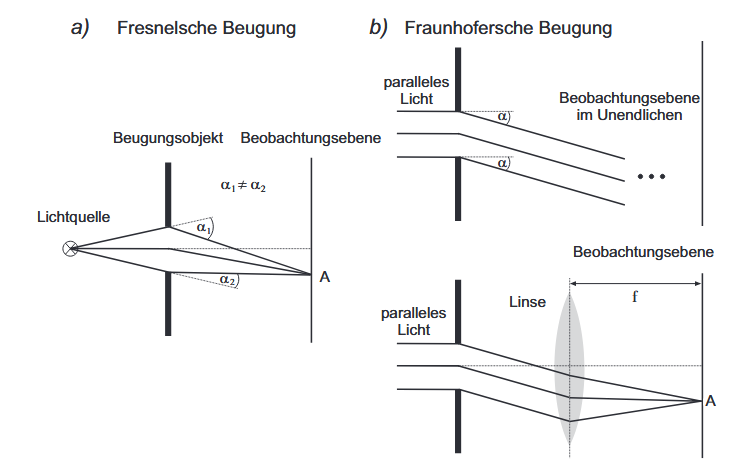
\includegraphics{graphics/fresnel und fraunhofer beugung.png}}
    \caption{Fresnelsche und Fraunhofersche Beugung [Quelle: PAP2.1 Skript, S.81, Stand: 02/2024]}
    \label{fig:fresnel_fraunhofer}
\end{figure}

Grundsätzlich gibt es zwei verschiedene Arten von Versuchsanordnungen, mit denen sich Beugungserscheinungen beobachten lassen: Fresnelsche Beugung und Fraunhofersche Beugung. Bei Ersterer liegen die Lichtquelle und Beobachtungsebene in einem endlichen Abstand von dem Beugenden Objekt entfernt, wodurch sich ein recht kompliziertes geometrisches Problem ergibt. Bei der Fraunhofer Beugung hingegen liegt die Lichtquelle im unendlichen, wodurch die Lichtstrahlen parallel auf das Objekt treffen und danach von einer Linse gesammelt werden. Wir werden hier nur mit Fraunhoferscher Beugung arbeiten und unsere Lichtquellen als unendlich weit entfernt annehmen, was eine akzeptable Näherung in unserem Versuchs ein wird. 

Betrachten wir beispielhaft die Beugung am Einzelspalt. Ein paralleler und monochromatische Lichtstrahl, der auf einen Spalt mit der Wellenlänge $\lambda$, der Amplitude $E_0$ und der Phase $\varphi = \omega t$ trifft, lässt sich folgendermaßen beschreiben:

\begin{equation}
    E(y) = E_0 e^{i\omega t}.
\end{equation}

\begin{figure}[!t]
    \centering
    \resizebox{0.9\textwidth}{!}{
    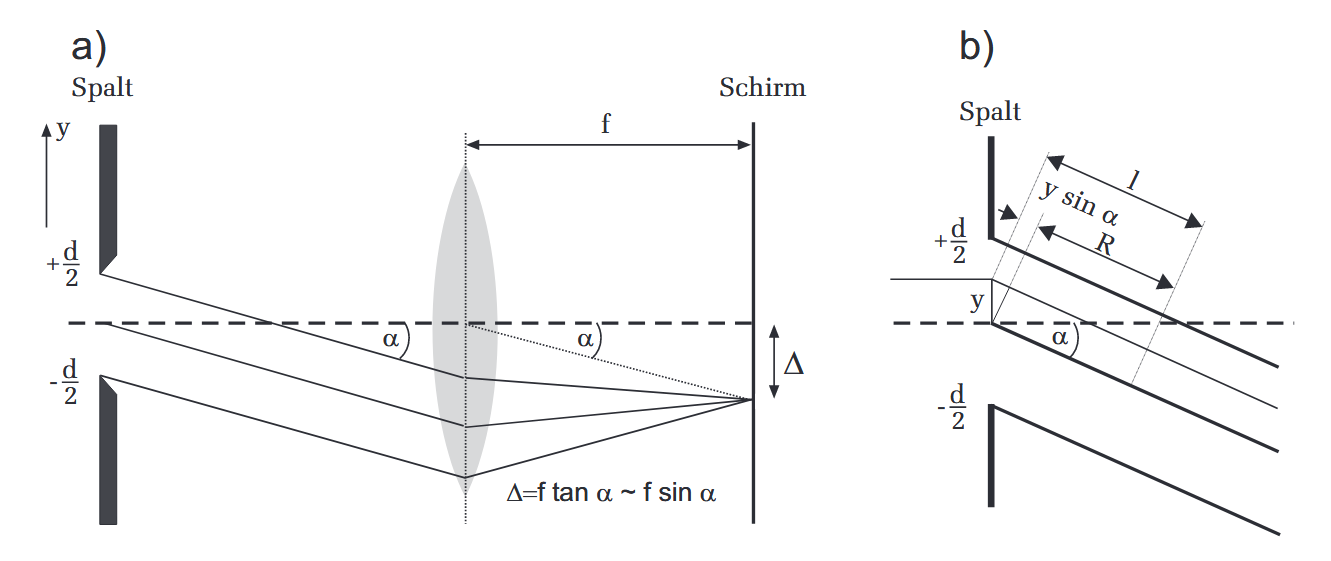
\includegraphics{graphics/fraunhofer beugung.png}}
    \caption{Fraunhofersche Beugung am Spalt [Quelle: PAP2.1 Skript, S.81, Stand: 02/2024]}
    \label{fig:fraunhofer}
\end{figure}

Bricht sich dieser an dem Spalt so ergibt sich nach dem Huygens-Fermat'schen Prinzip für den Strahl in Richtung $\alpha$ hinter dem Spalt:

\begin{equation}
    E_\infty (\alpha) = \int^{d/2}_{d/2} E_0 e^{i(\omega t - kl)} dy.
\end{equation}

Hierbei sind $k = 2\pi / \lambda$ der Betrag des Wellenvektors und $l = R + y \sin{\alpha}$ die Weglänge des Lichtbündels. Das Integral ergibt mit der Abkürzung $x = (d/2) \pi \sin{\alpha}$:

\begin{equation}
    E_\infty (x) = E_0 e^{i(\omega t - kR)} \frac{\sin{x}}{x} d.
\end{equation}

Hieraus ergibt sich bei quadrieren die Intensität, welche das Beugungsbild des Einzelspalts darstellt:

\begin{equation}
    I_\infty (x) \propto d^2 \frac{\sin^2{x}}{x^2} \propto I_0^2 \frac{\sin^2{x}}{x^2}.
\end{equation}

\subsubsection{Fourierreihe und Fourierintegrale}

Jede periodische Funktion lässt sich als Fourierreihe mit den Fourierkoeffizienten $a_n$ und $b_n$ darstellen. Bei der Periode $L$ gilt für eine Funktion $f(x)$:

\begin{equation}
    \begin{split}
        f(x) &= \frac{a_0}{2} + \sum_{n=1}^\infty a_n \cos{\left( \frac{2 \pi n}{L} x \right)} + b_n \sin{\left( \frac{2 \pi n}{L} x \right)} \\ \\
        a_n &= \frac{2}{L} \int_{-L/2}^{L/2} f(x) \ \cos{\left( \frac{2 \pi n}{L} x \right)} \ dx \\ \\
        b_n &= \frac{2}{L} \int_{-L/2}^{L/2} f(x) \ \sin{\left( \frac{2 \pi n}{L} x \right)} \ dx
    \end{split}
\end{equation}

Ebenso kann man aber auch nichtperiodische Funktionen in einer Fourierreihe im Grenzwert von $L \xrightarrow[]{} \infty$ darstellen, wobei die Reihe hierbei in ein Integral übergeht und man die Fouriertransformation einer Funktion $f(x)$ zur Fouriertransformierten $\mathcal{F}(k)$ erhält:

\begin{equation}
    \begin{split}
        f(x) &= \int_\infty^\infty \mathcal{F}(k) e^{ikx} dk \\ \\
        \mathcal{F}(k) &= \frac{1}{2 \pi } \int_\infty^\infty f(x) e^{-ikx} dx
    \end{split}
\end{equation}

Eine wichtige Schlussfolgerung, die in Literatur hergeleitet, hier aber nur genannt und angewendet werden soll, ist, dass die Feldverteilung der Fraunhofer'schen Beugung an einer Öffnung genau die Fouriertransformierte der Feldverteilung über die beugende Öffnung entspricht. Ergo, die Fouriertransformation einer Funktion, welche die Öffnung an der gebeugt wird beschreibt, liefert uns das erwartete Beugungsbild dieser Öffnung. Diese Erkenntnis wird Grundlage dieses Versuchs und der nächsten zwei Kapitel sein, wo mit diesem Ansatz die Beugungsfunktionen des Einzel- und Doppelspalts hergeleitet werden sollen.

\subsubsection{Fouriertransformierte des Einzelspalts}

Ein Einzelspalt der Breite $d$ lässt sich mit folgender Spaltfunktion beschreiben:

\begin{equation}
    f(x) =
    \begin{cases} 
    \vert 1 , & |y| \leq d / 2 \\
    \vert 0 , & |y| > d / 2 \\
    \end{cases}.
\end{equation}

Damit ergibt sich aus der Fouriertransformation:

\begin{equation}
    \begin{split}
        \mathcal{F}(k_y) &= d \frac{\sin{(k_y d/2)}}{k_y d/2}, \\ \\
        \Rightarrow I(k_y) &= d^2 \frac{\sin^2{(k_y d/2)}}{(k_y d/2)^2}.
    \end{split}
\end{equation}

Die Nullstellen dieser Funktion liegen bei $k_y = {2 \pi n}/{d}$. Ebenso kann man aus dieser Fouriertransformierten nun rückwärtig die Spaltfunktion erhalten, wobei sich das folgende Integral ergibt:

\begin{equation}
    f (y) = \frac{d}{\pi} \int_0^{k_{y,n}} \frac{\sin{(k_y d / 2)}}{k_y d / 2} \ \cos{(k_y y)} \ dk_y
\end{equation}

Dieses Integral ist nicht analytisch lösbar und muss durch eine numerische Integration gelöst werden, wobei die obere Integrationsgrenze $k_{y,n}$ bestimmt, wie viele Ordnungen $n$ zum Objektbild zugelassen werden. Für $k_{y,n} = + \infty$ ergibt sich einfach das normale Spaltbild. Jedoch kann man auch die $n$-te Nullstelle von $\mathcal{F}$ als Integrationsgrenze wählen, was vor allem für uns interessant ist, da wir in diesem Versuch gezielt Nebenmaxima des Beugungsbilds eines Spalts abschneiden und dabei Veränderungen im Objektbild untersuchen werden. Hier gilt:

\begin{equation}
    k_{y,n} = k_0 \sin{(\alpha_n)} = k_0 n \frac{\lambda}{d} = 2 n \frac{\pi}{d}.
    \label{eq:01_k_yn}
\end{equation}

\begin{figure}[h]
  \centering
  \subfloat[Einzelspalt]{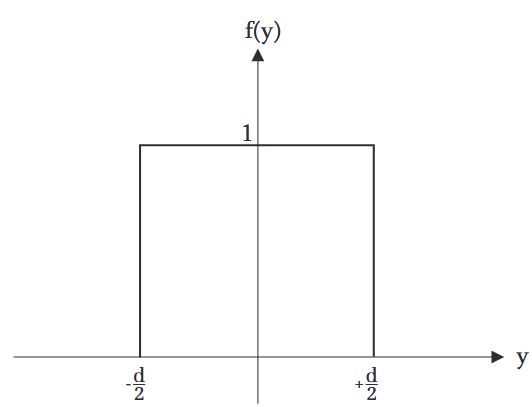
\includegraphics[width=0.48\textwidth]{graphics/einzelspalt.png}}
  \hfill
  \subfloat[Doppelspalt]{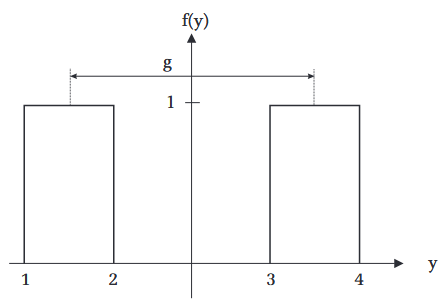
\includegraphics[width=0.48\textwidth]{graphics/doppelspalt.png}}
  \hfill
  \caption{Spaltfunktionen [Quelle: PAP2.1 Skript, S.88 \& 90, Stand: 02/2024]}
  \label{fig:Spaltfunktionen}
\end{figure}

\newpage
\subsubsection{Fouriertransformierte des Doppelspalts}

Für den Doppelspalt geht man analog zum Einzelspalt vor. Die Spaltfunktion bei Spaltbreite $d$ und Spaltabstand $g$ ist in Abbildung \ref{fig:Spaltfunktionen} dargestellt. Die Fouriertransformierte ergibt sich hierbei als:

\begin{equation}
    \begin{split}
        \mathcal{F}(k_y) &= 2d \ \cos{(k_y g/2)} \ \frac{\sin{(k_y d/2)}}{k_y d/2}, \\ \\
        \Rightarrow I(k_y) &= 4d^2 \ \cos^2{(k_y g/2)} \ \frac{\sin^2{(k_y d/2)}}{(k_y d/2)^2}.
    \end{split}
\end{equation}

Aus der Rücktransformation ergeben sich auch hier wieder die modifizierten Bilder, für den Fall dass nur eine endliche Zahl an Nebenmaxima zugelassen werden:

\begin{equation}
    f_{mod,d} (y) = \frac{2d}{\pi} \int_0^{k_{y,n}} \frac{\sin{(k_y d / 2)}}{k_y d / 2} \ \cos{(k_y y)} \ \cos{(k_y g / 2)} \ dk_y.
\end{equation}

Allgemein gelten hier dieselben Formeln für $k_{y,n}$ wie beim Einzespalt.

\newpage
\subsection{Versuchsaufbau}

Der Versuchsaufbau, zu sehen in Abbildung \ref{fig:Aufbau} sowohl als Foto als auch als Skizze, lässt sich grunlegend folgendermaßen beschreiben: Ein Laser bestrahlt ein Objekt, beispielsweise einen Einzel- oder Doppelspalt, woraufhin das Beugungsbild von der Linse L1 im Brennpunkt dieser Linse 80mm hintendran gesammelt wird. In dieser sogenannten Fourierebene ist ein Analysespalt angebracht, welcher in der Breite so eingestellt werden kann, dass die äußeren Nebenmaxima des Beugungsbilds abgeschnitten werden können. Dahinter befindet sich ein Strahlenteiler, welcher Beugungsbild und Objektbild voneinander trennt. Ersteres wird über eine weitere Linse L2 sowie einen Spiegel auf einen Schirm beziehungsweise die Kamera zur Beobachtung geleitet, während das Objektbild im Strahlengang einfach geraudeaus auf gleiche weiterlaufen kann. Vor dem Laser befindet sich zum Schutz der Kamera ein Graulichtfilter, der in den Strahlengang geklappt werden kann und die Intensität des Lasers erheblich reduziert. Manuelle Beobachtungen mit bloßem auge finden also ohne und Kameraufnahmen mit diesem statt. 

Es werden noch die Programme Thorcam zur Aufnahme der Bilder der Kamera sowie Gwyddion zur Maskierung der Bilder und Erstellung der Intensitätsprofile verwendet. 

\begin{figure}[!bp]
  \centering
  \subfloat{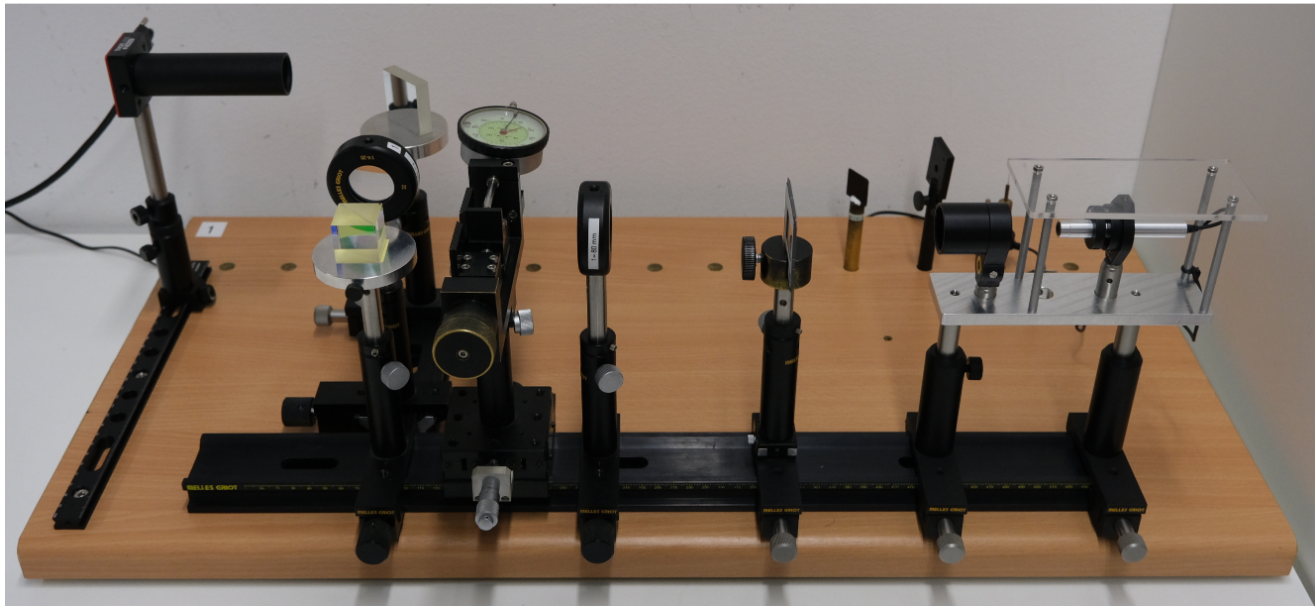
\includegraphics[width=0.6\textwidth]{graphics/aufbau foto.png}}
  \hfill
  \subfloat{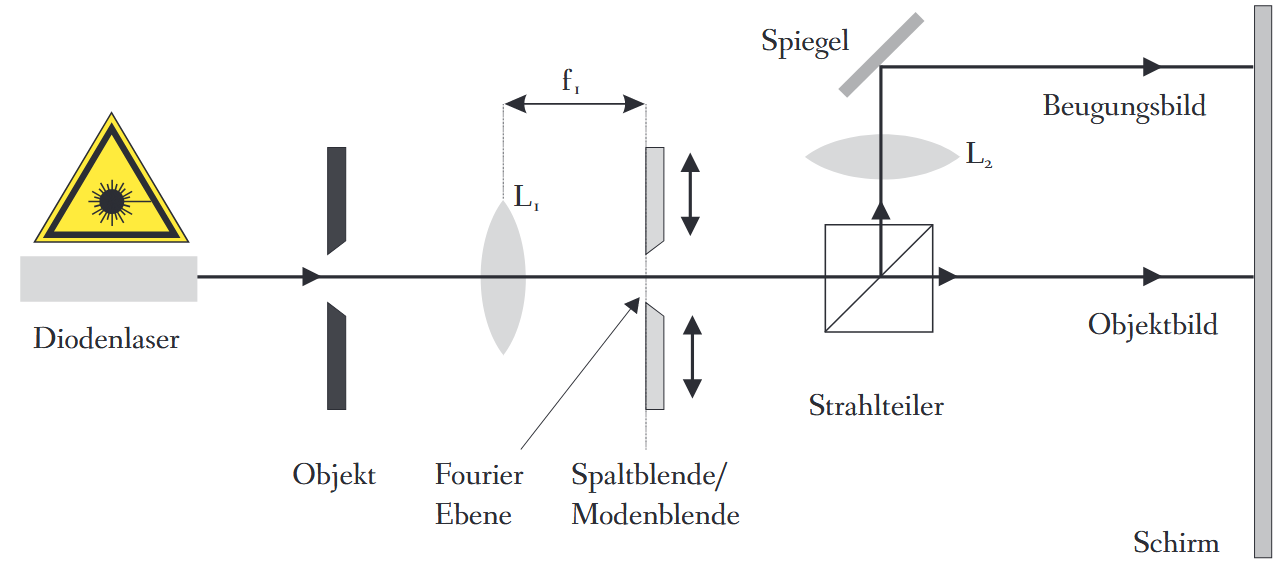
\includegraphics[width=0.6\textwidth]{graphics/aufbau schema.png}}
  \hfill
  \caption{Versuchsaufbau [Quelle: PAP2.1 Skript, S.79 \& 80, Stand: 02/2024]}
  \label{fig:Aufbau}
\end{figure}


\clearpage
%---------------VERSUCHSPROTOKOLL MIT MESSDATEN---------------
\newpage

\section{Versuchsprotokoll mit Messdaten}

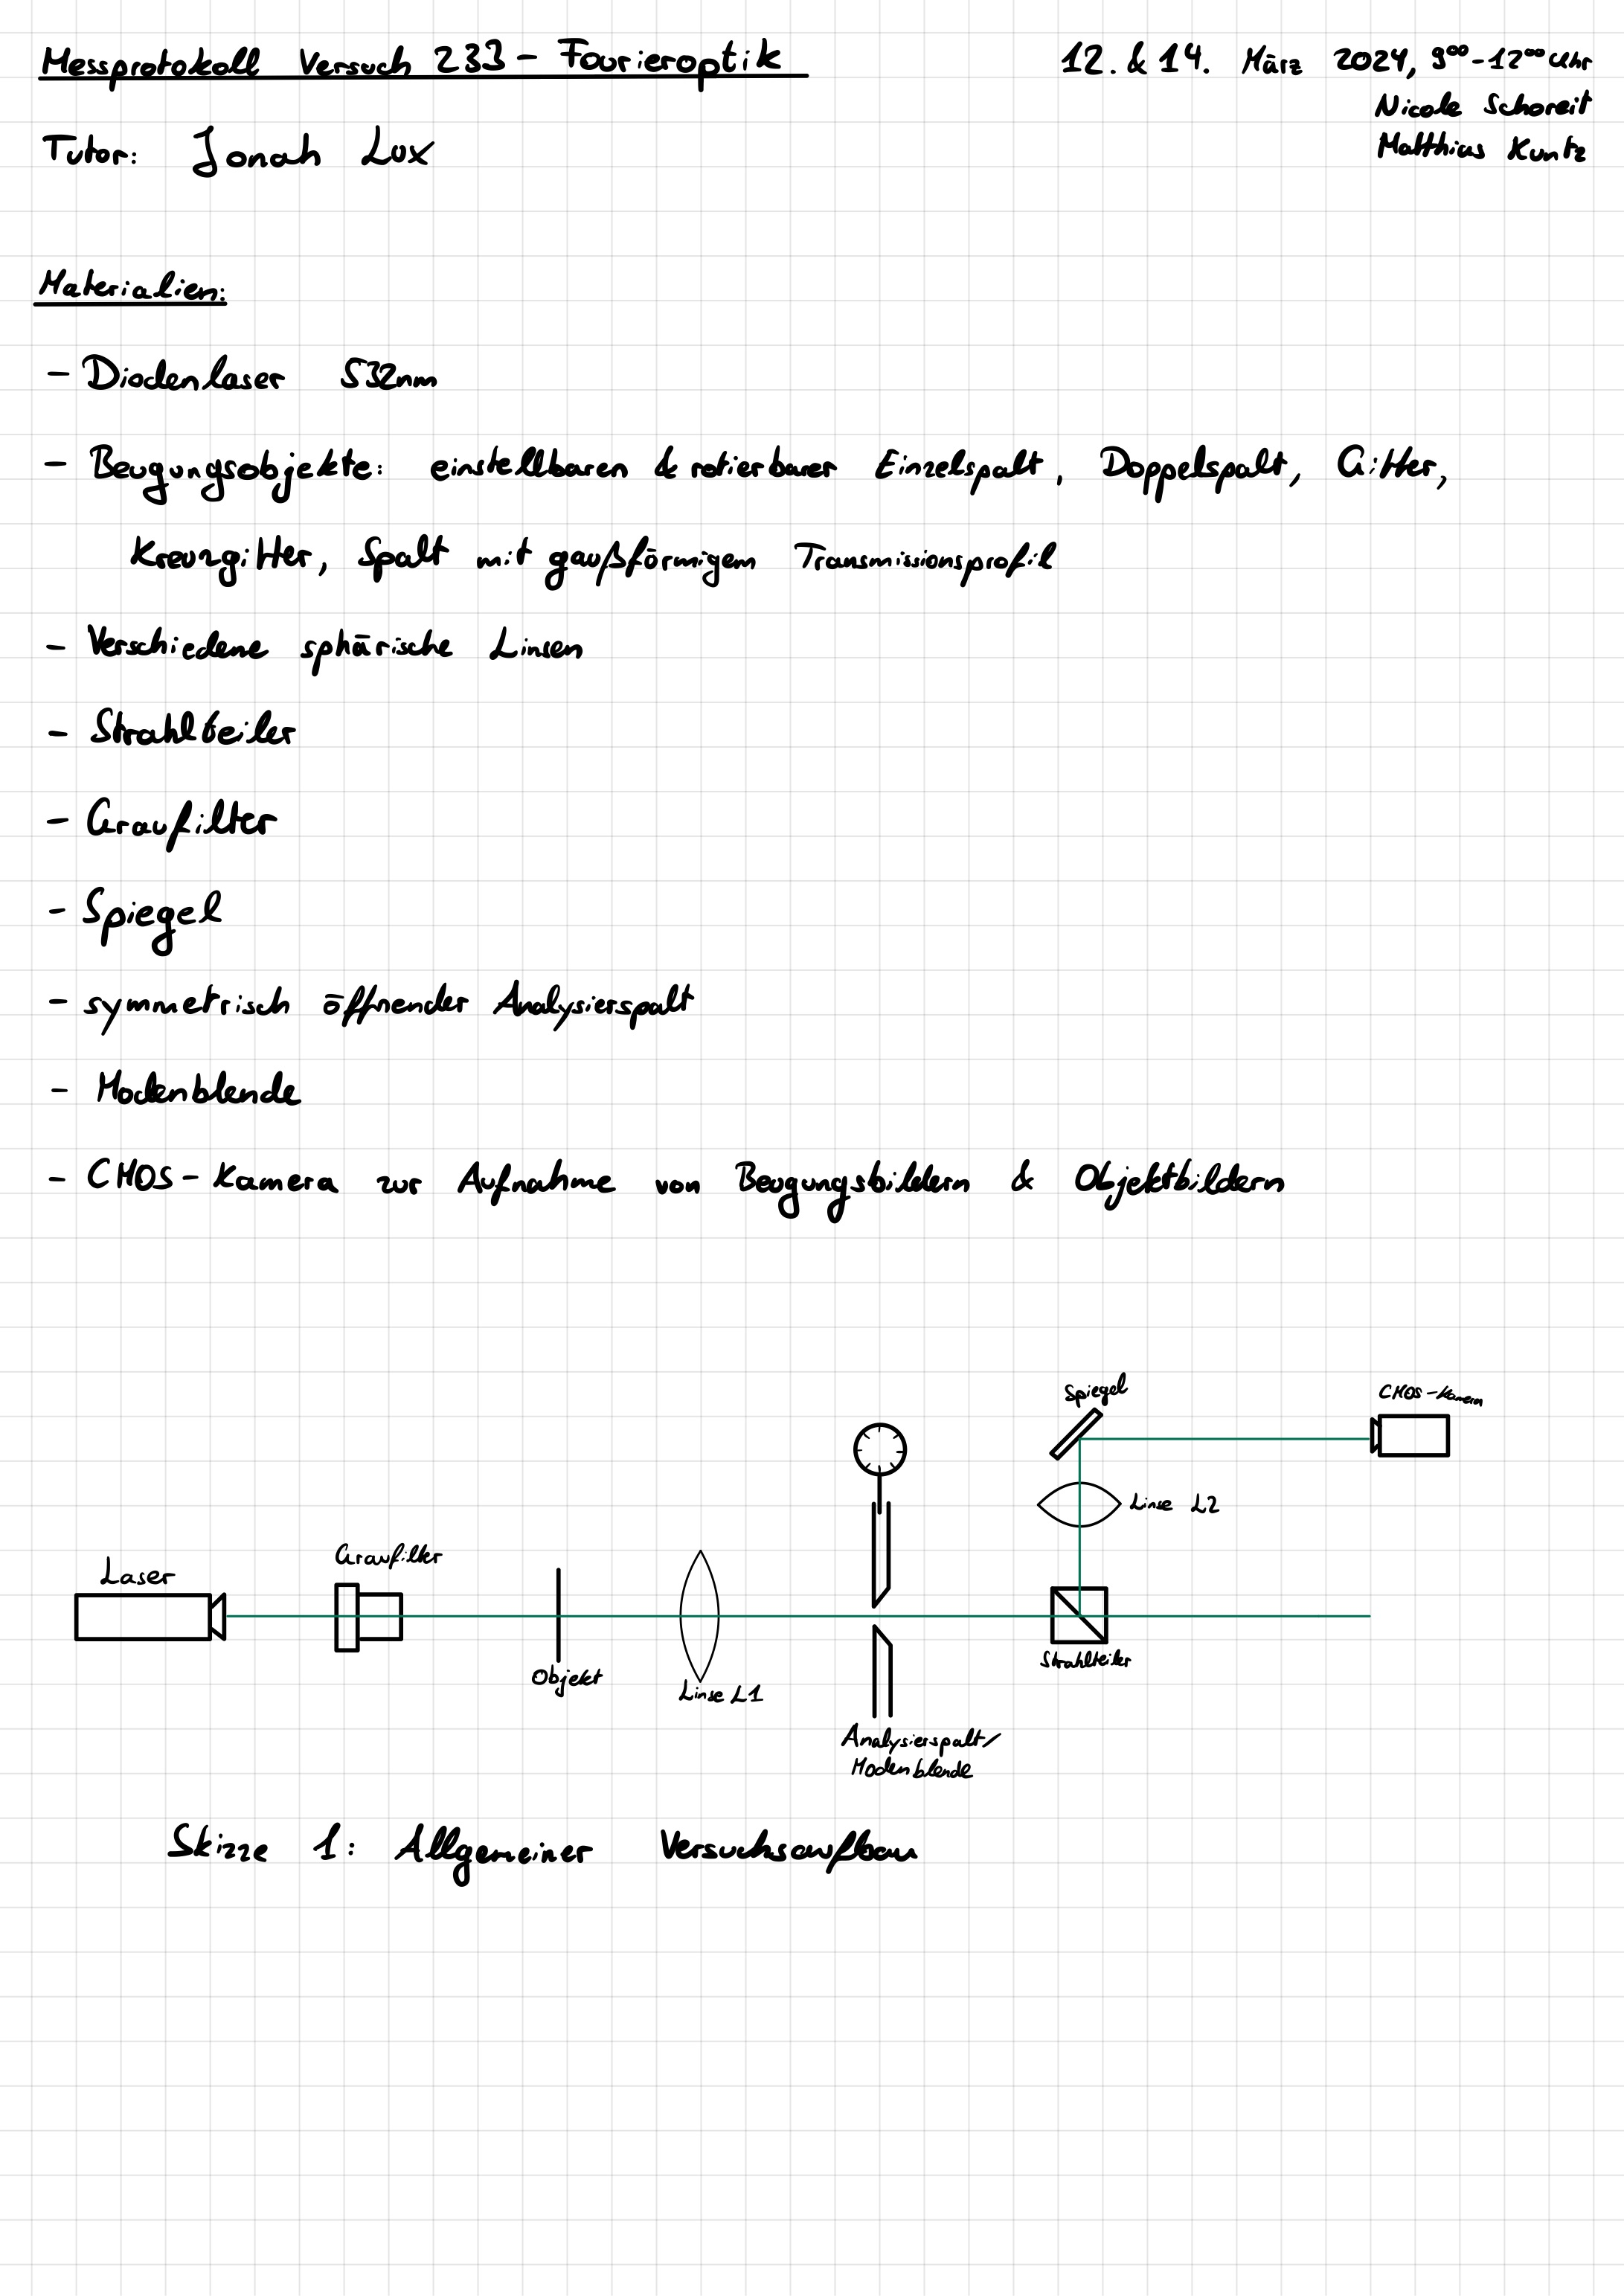
\includegraphics[width=\textwidth]{graphics/messprotokoll/233 - Fourieroptik-3.jpg}
\newpage
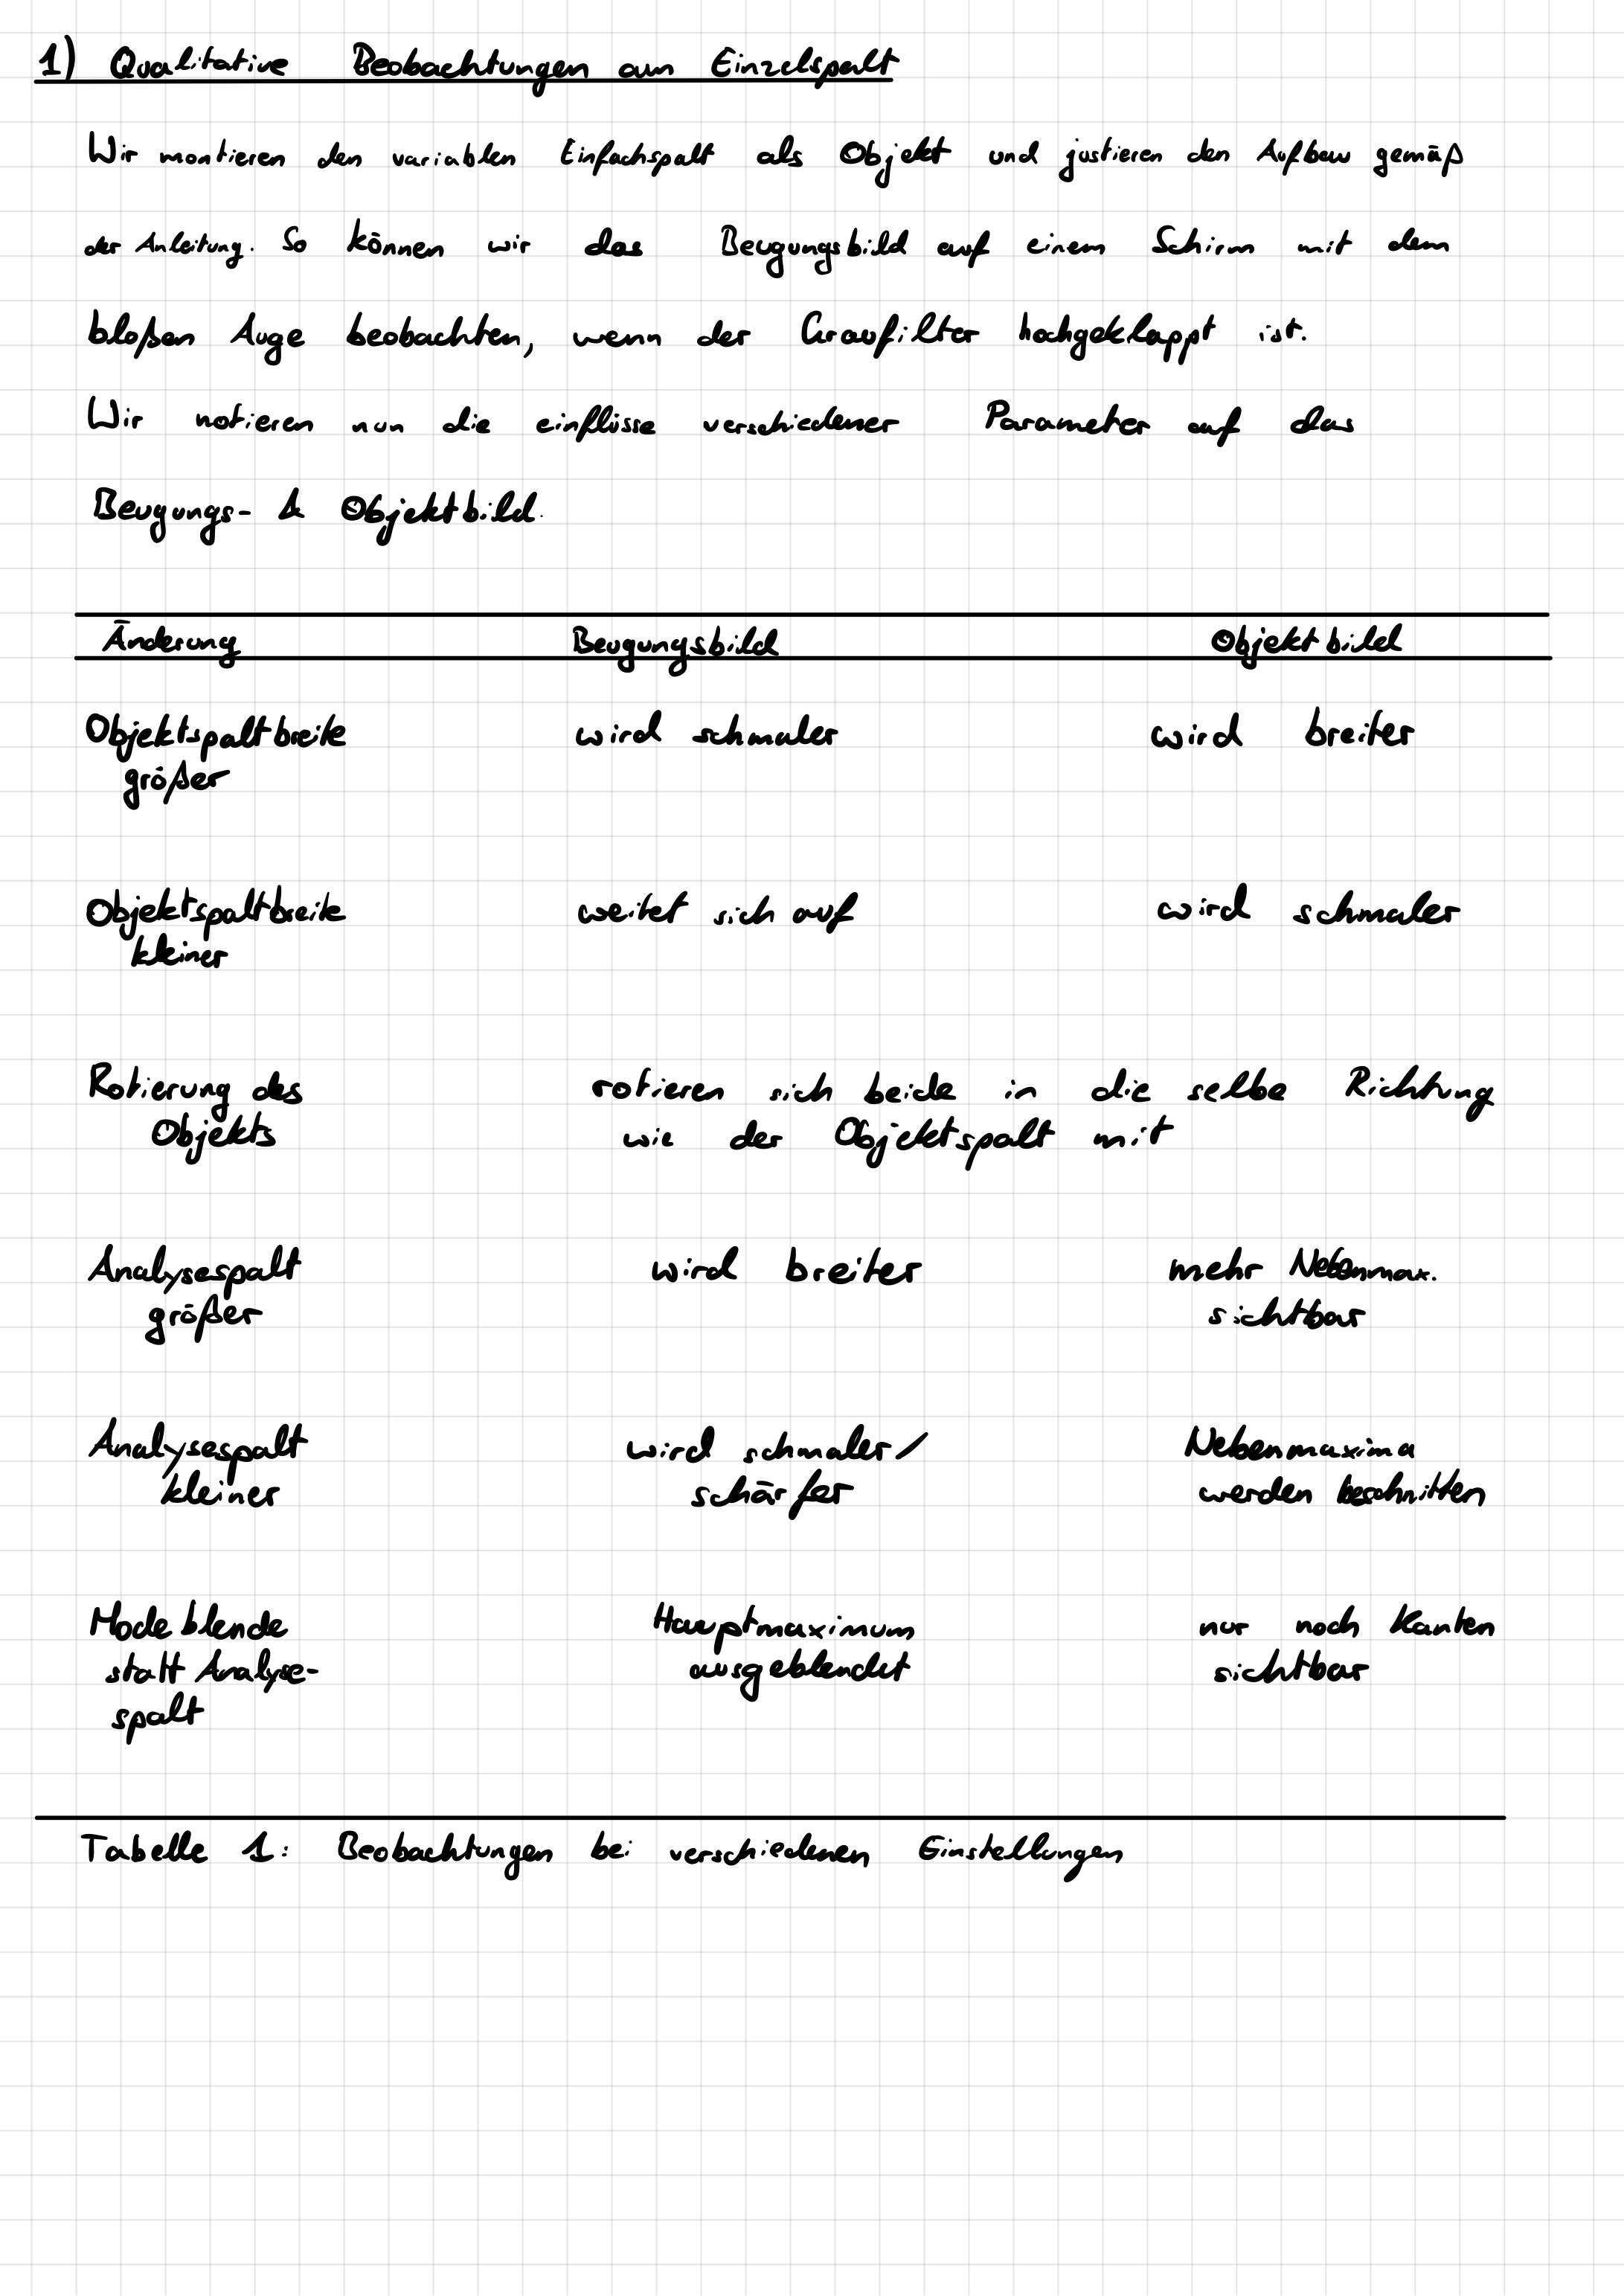
\includegraphics[width=\textwidth]{graphics/messprotokoll/233 - Fourieroptik-4.jpg}
\newpage
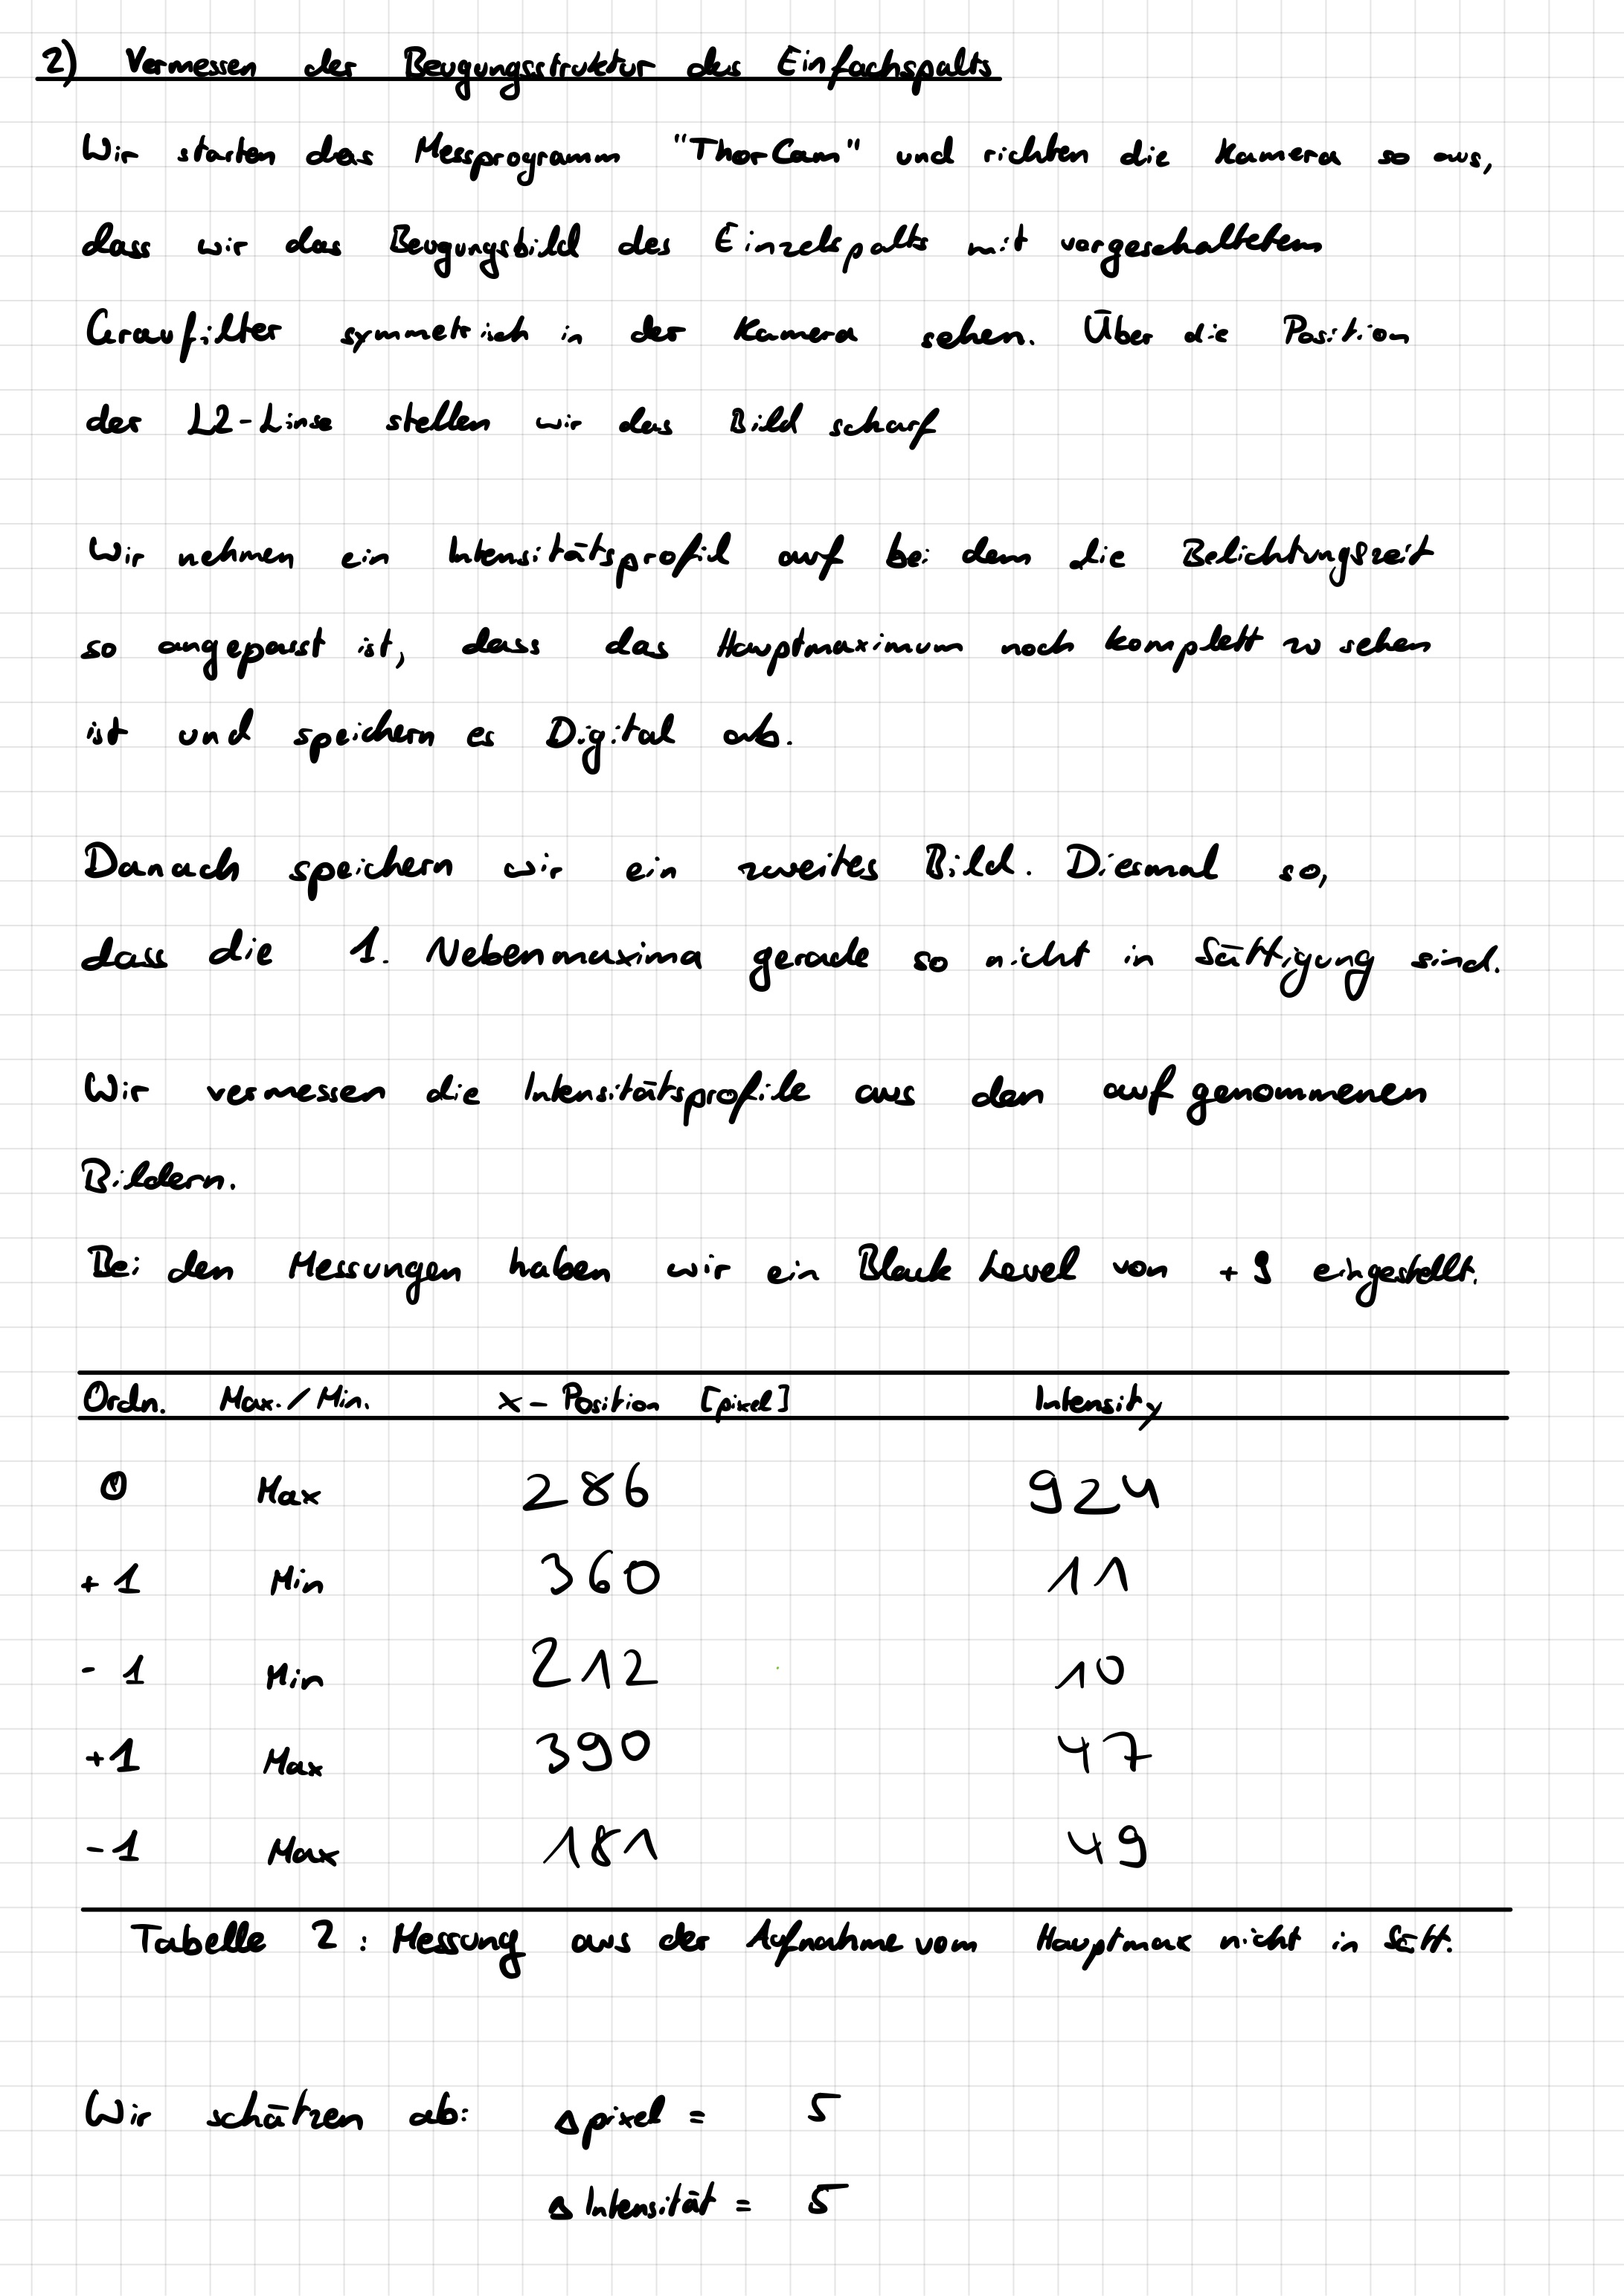
\includegraphics[width=\textwidth]{graphics/messprotokoll/233 - Fourieroptik-5.jpg}
\newpage
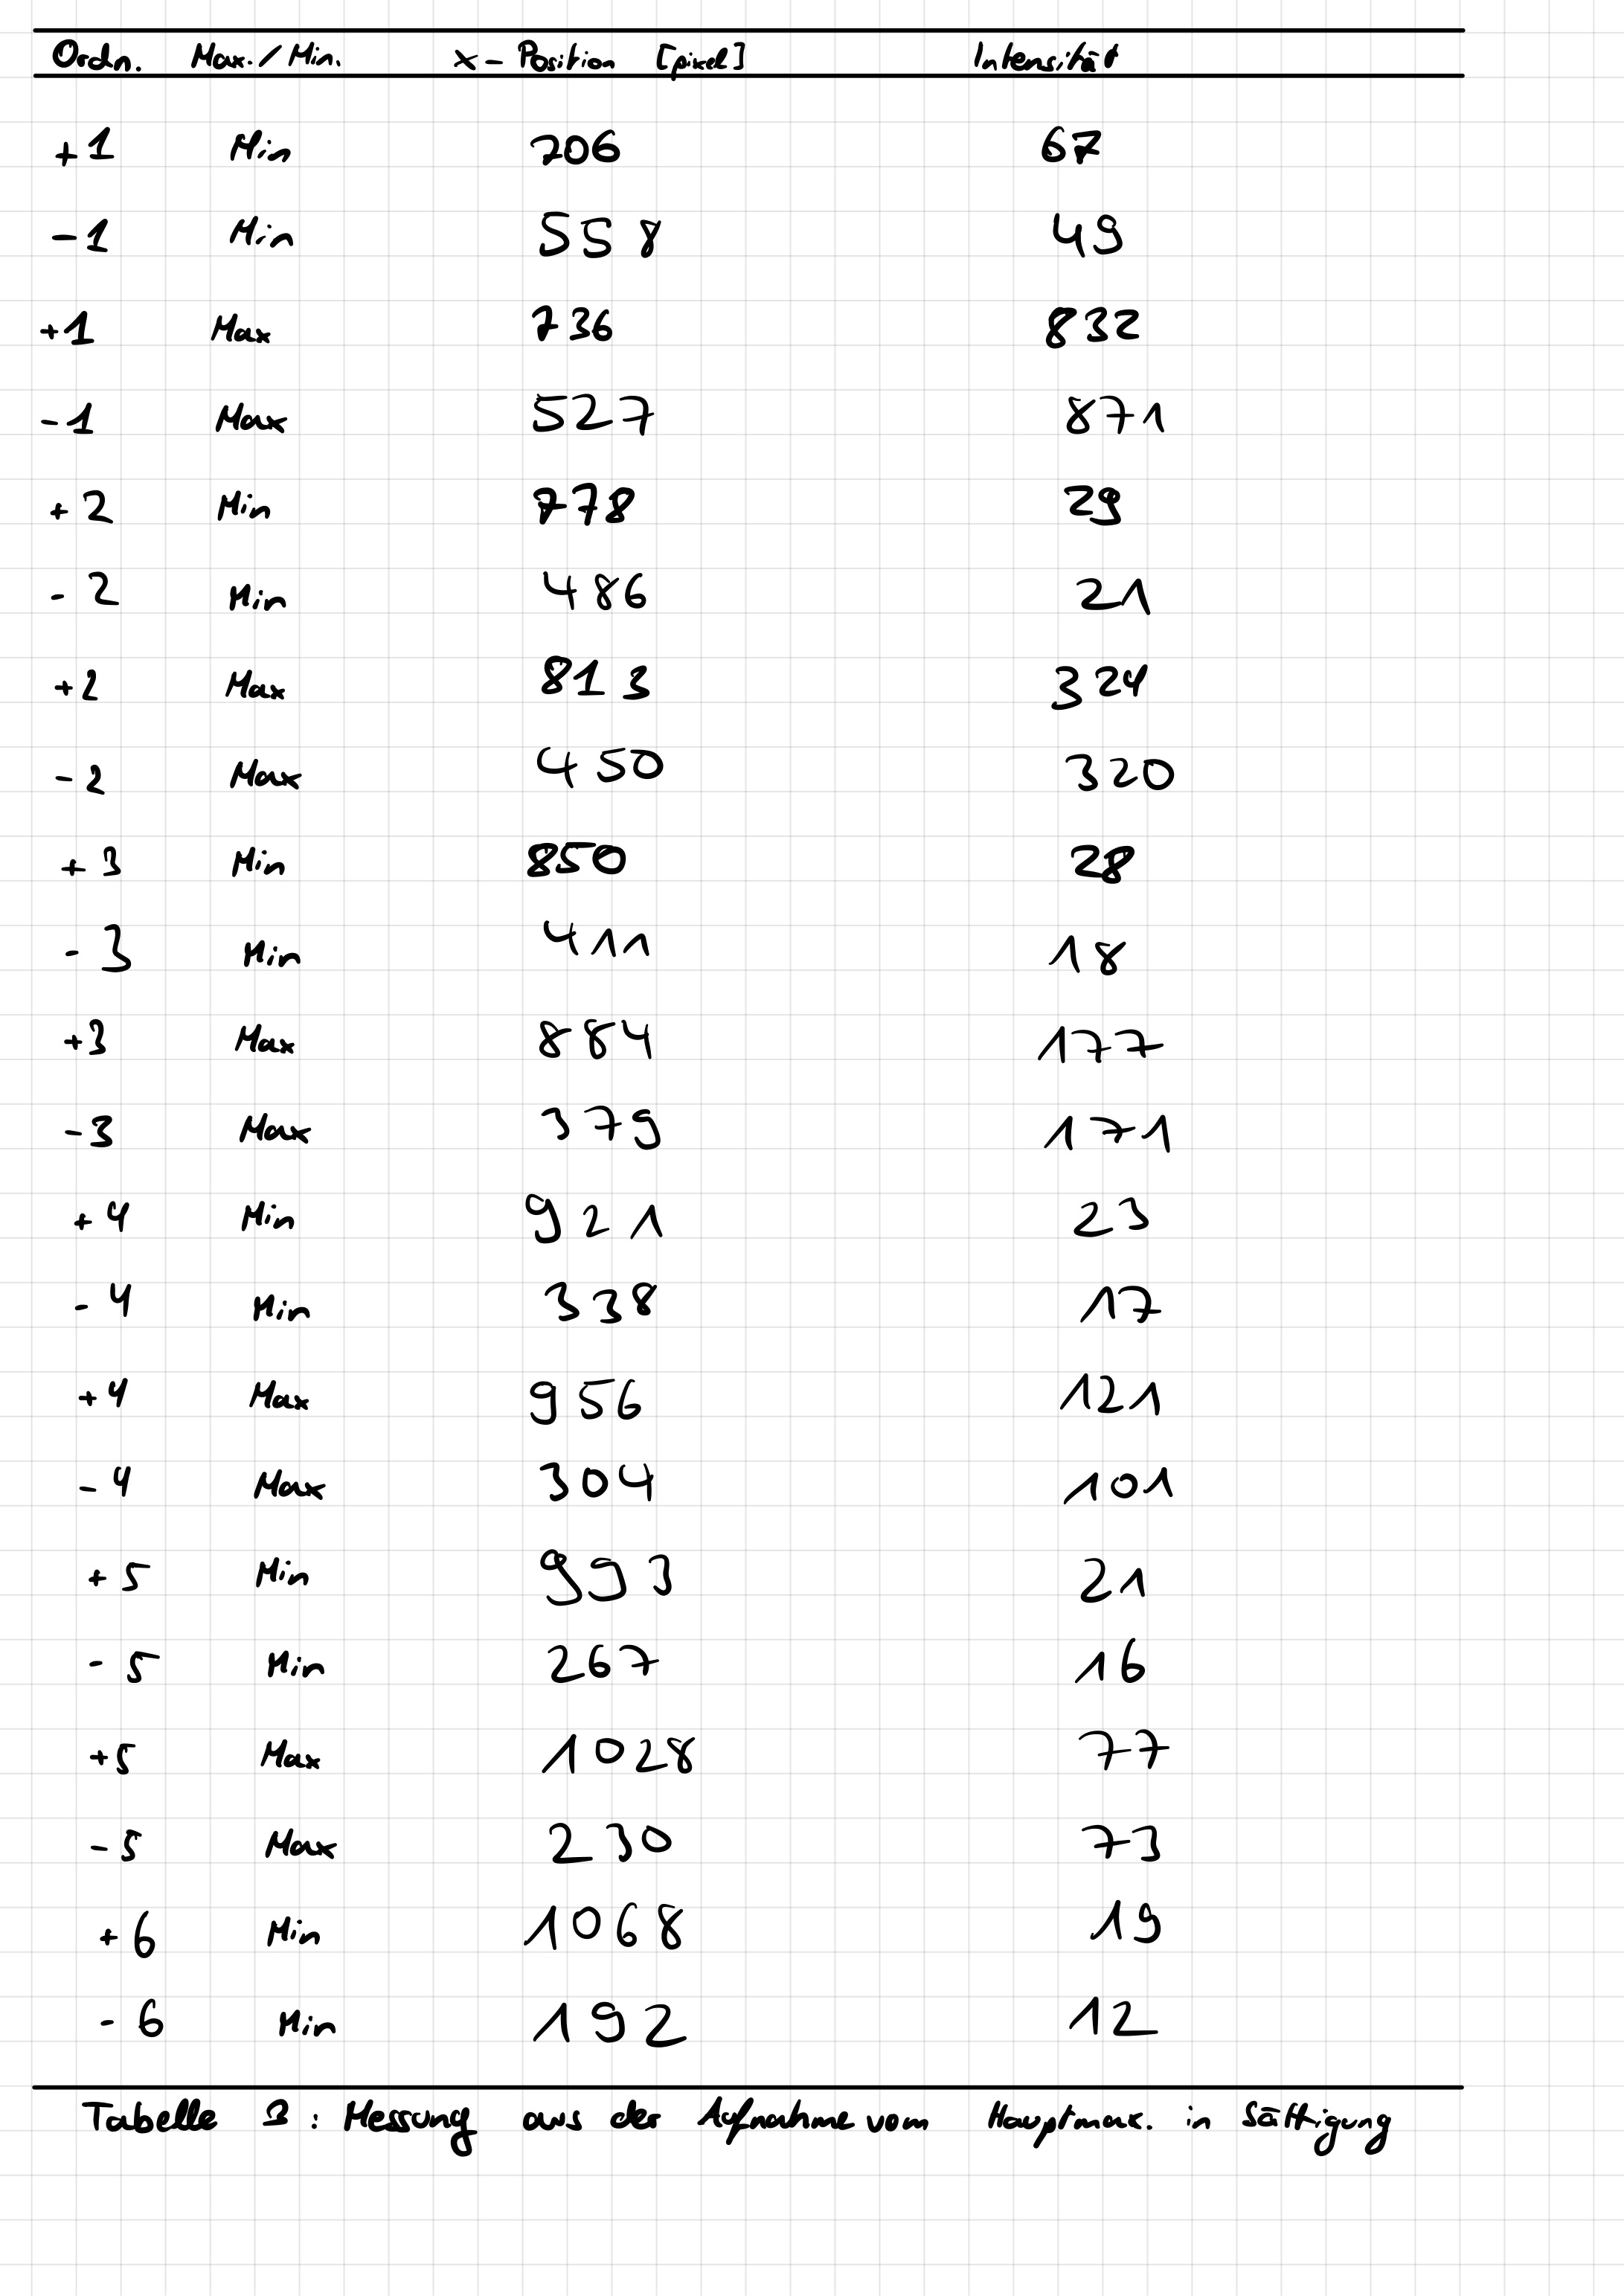
\includegraphics[width=\textwidth]{graphics/messprotokoll/233 - Fourieroptik-6.jpg}
\newpage
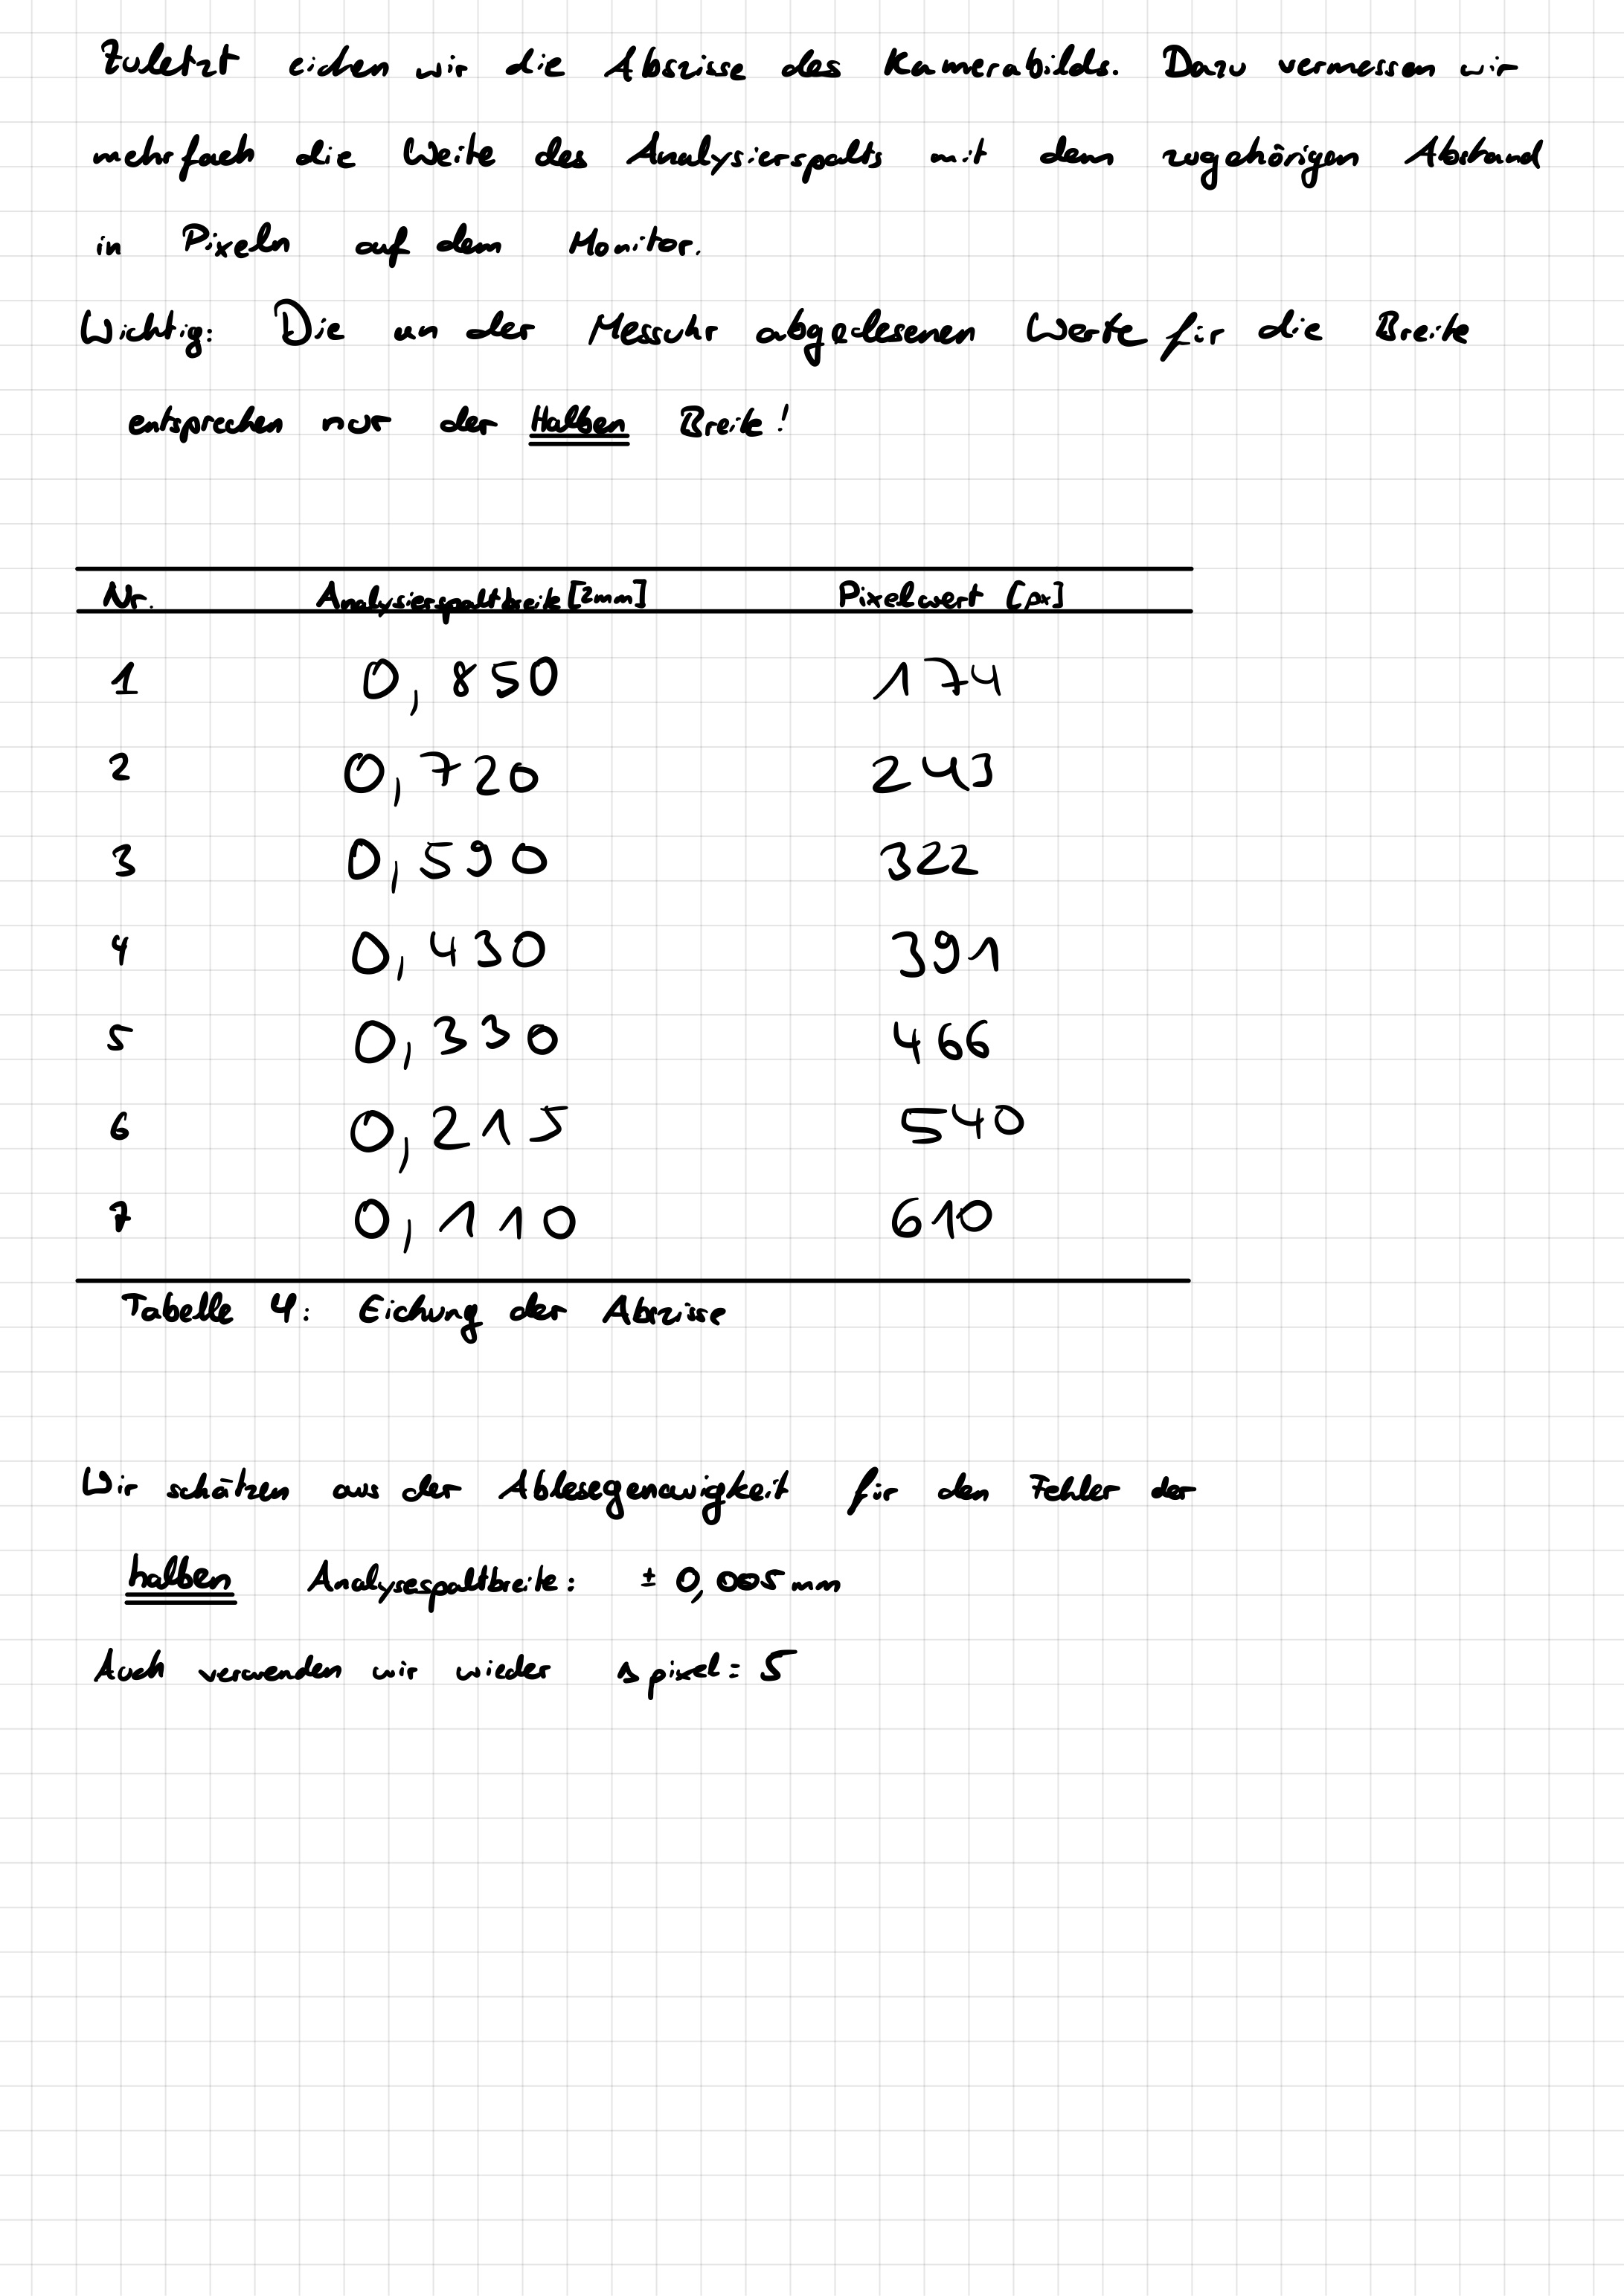
\includegraphics[width=\textwidth]{graphics/messprotokoll/233 - Fourieroptik-7.jpg}
\newpage
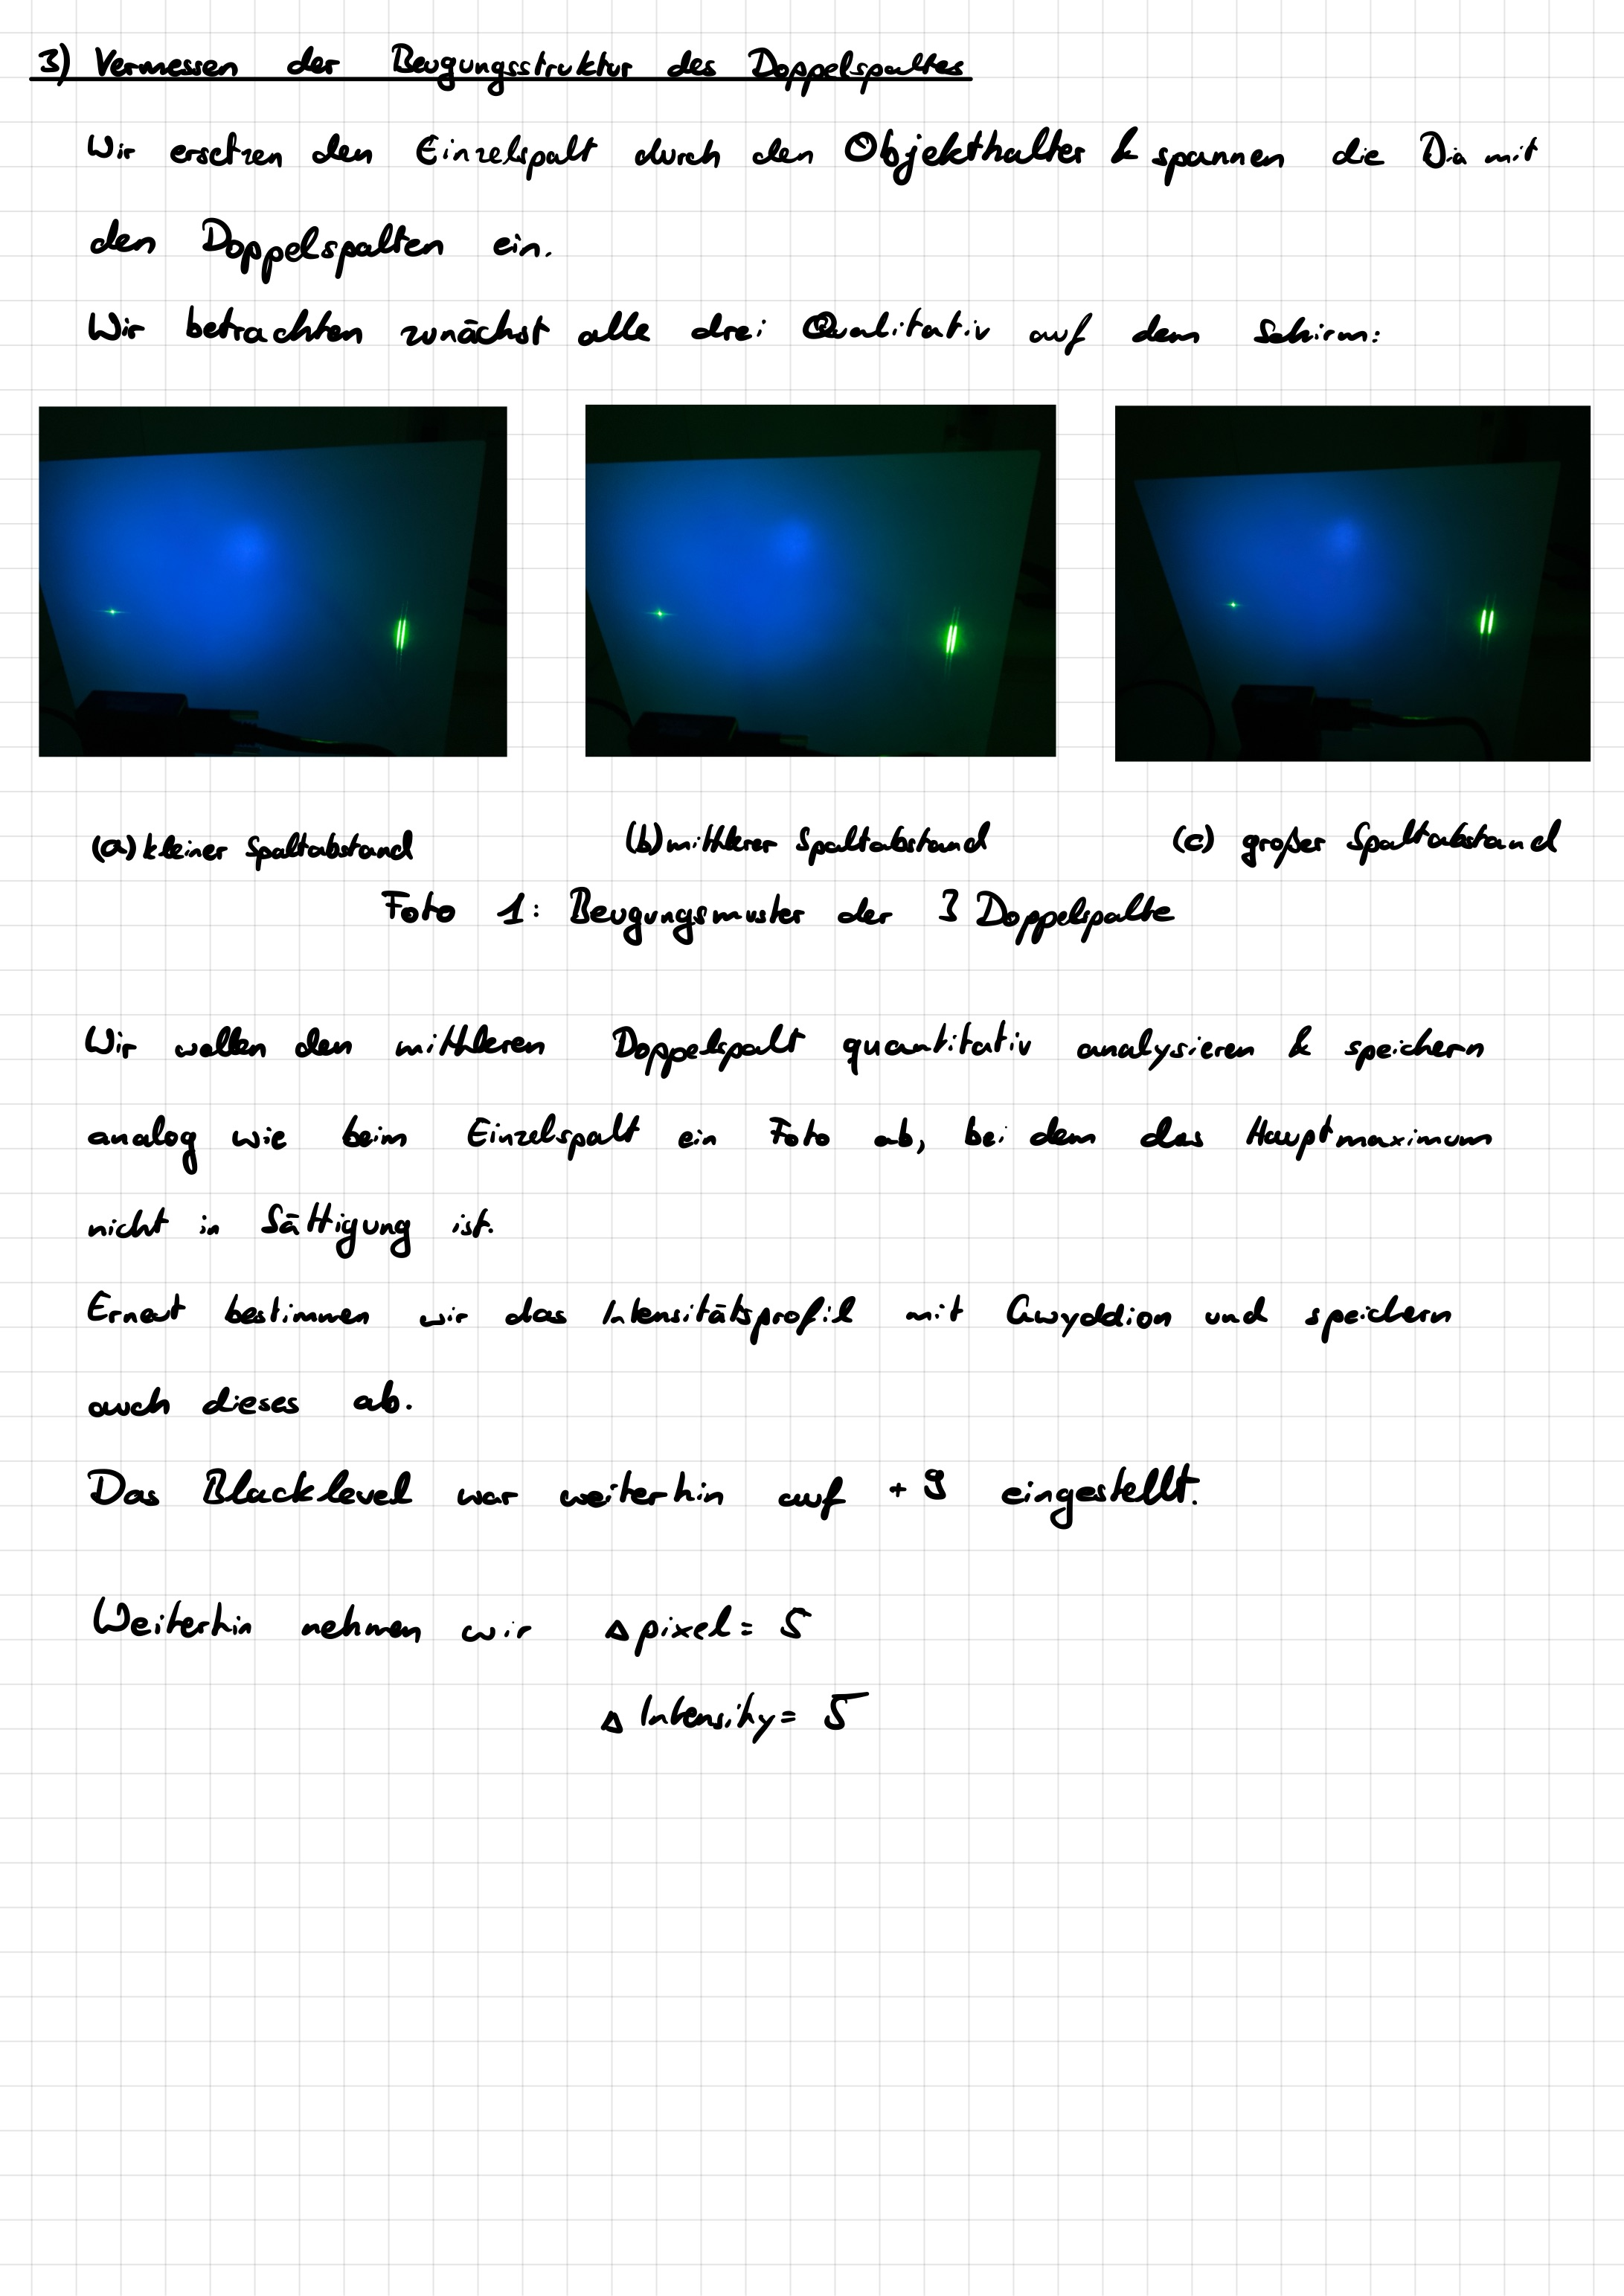
\includegraphics[width=\textwidth]{graphics/messprotokoll/233 - Fourieroptik-8.jpg}
\newpage
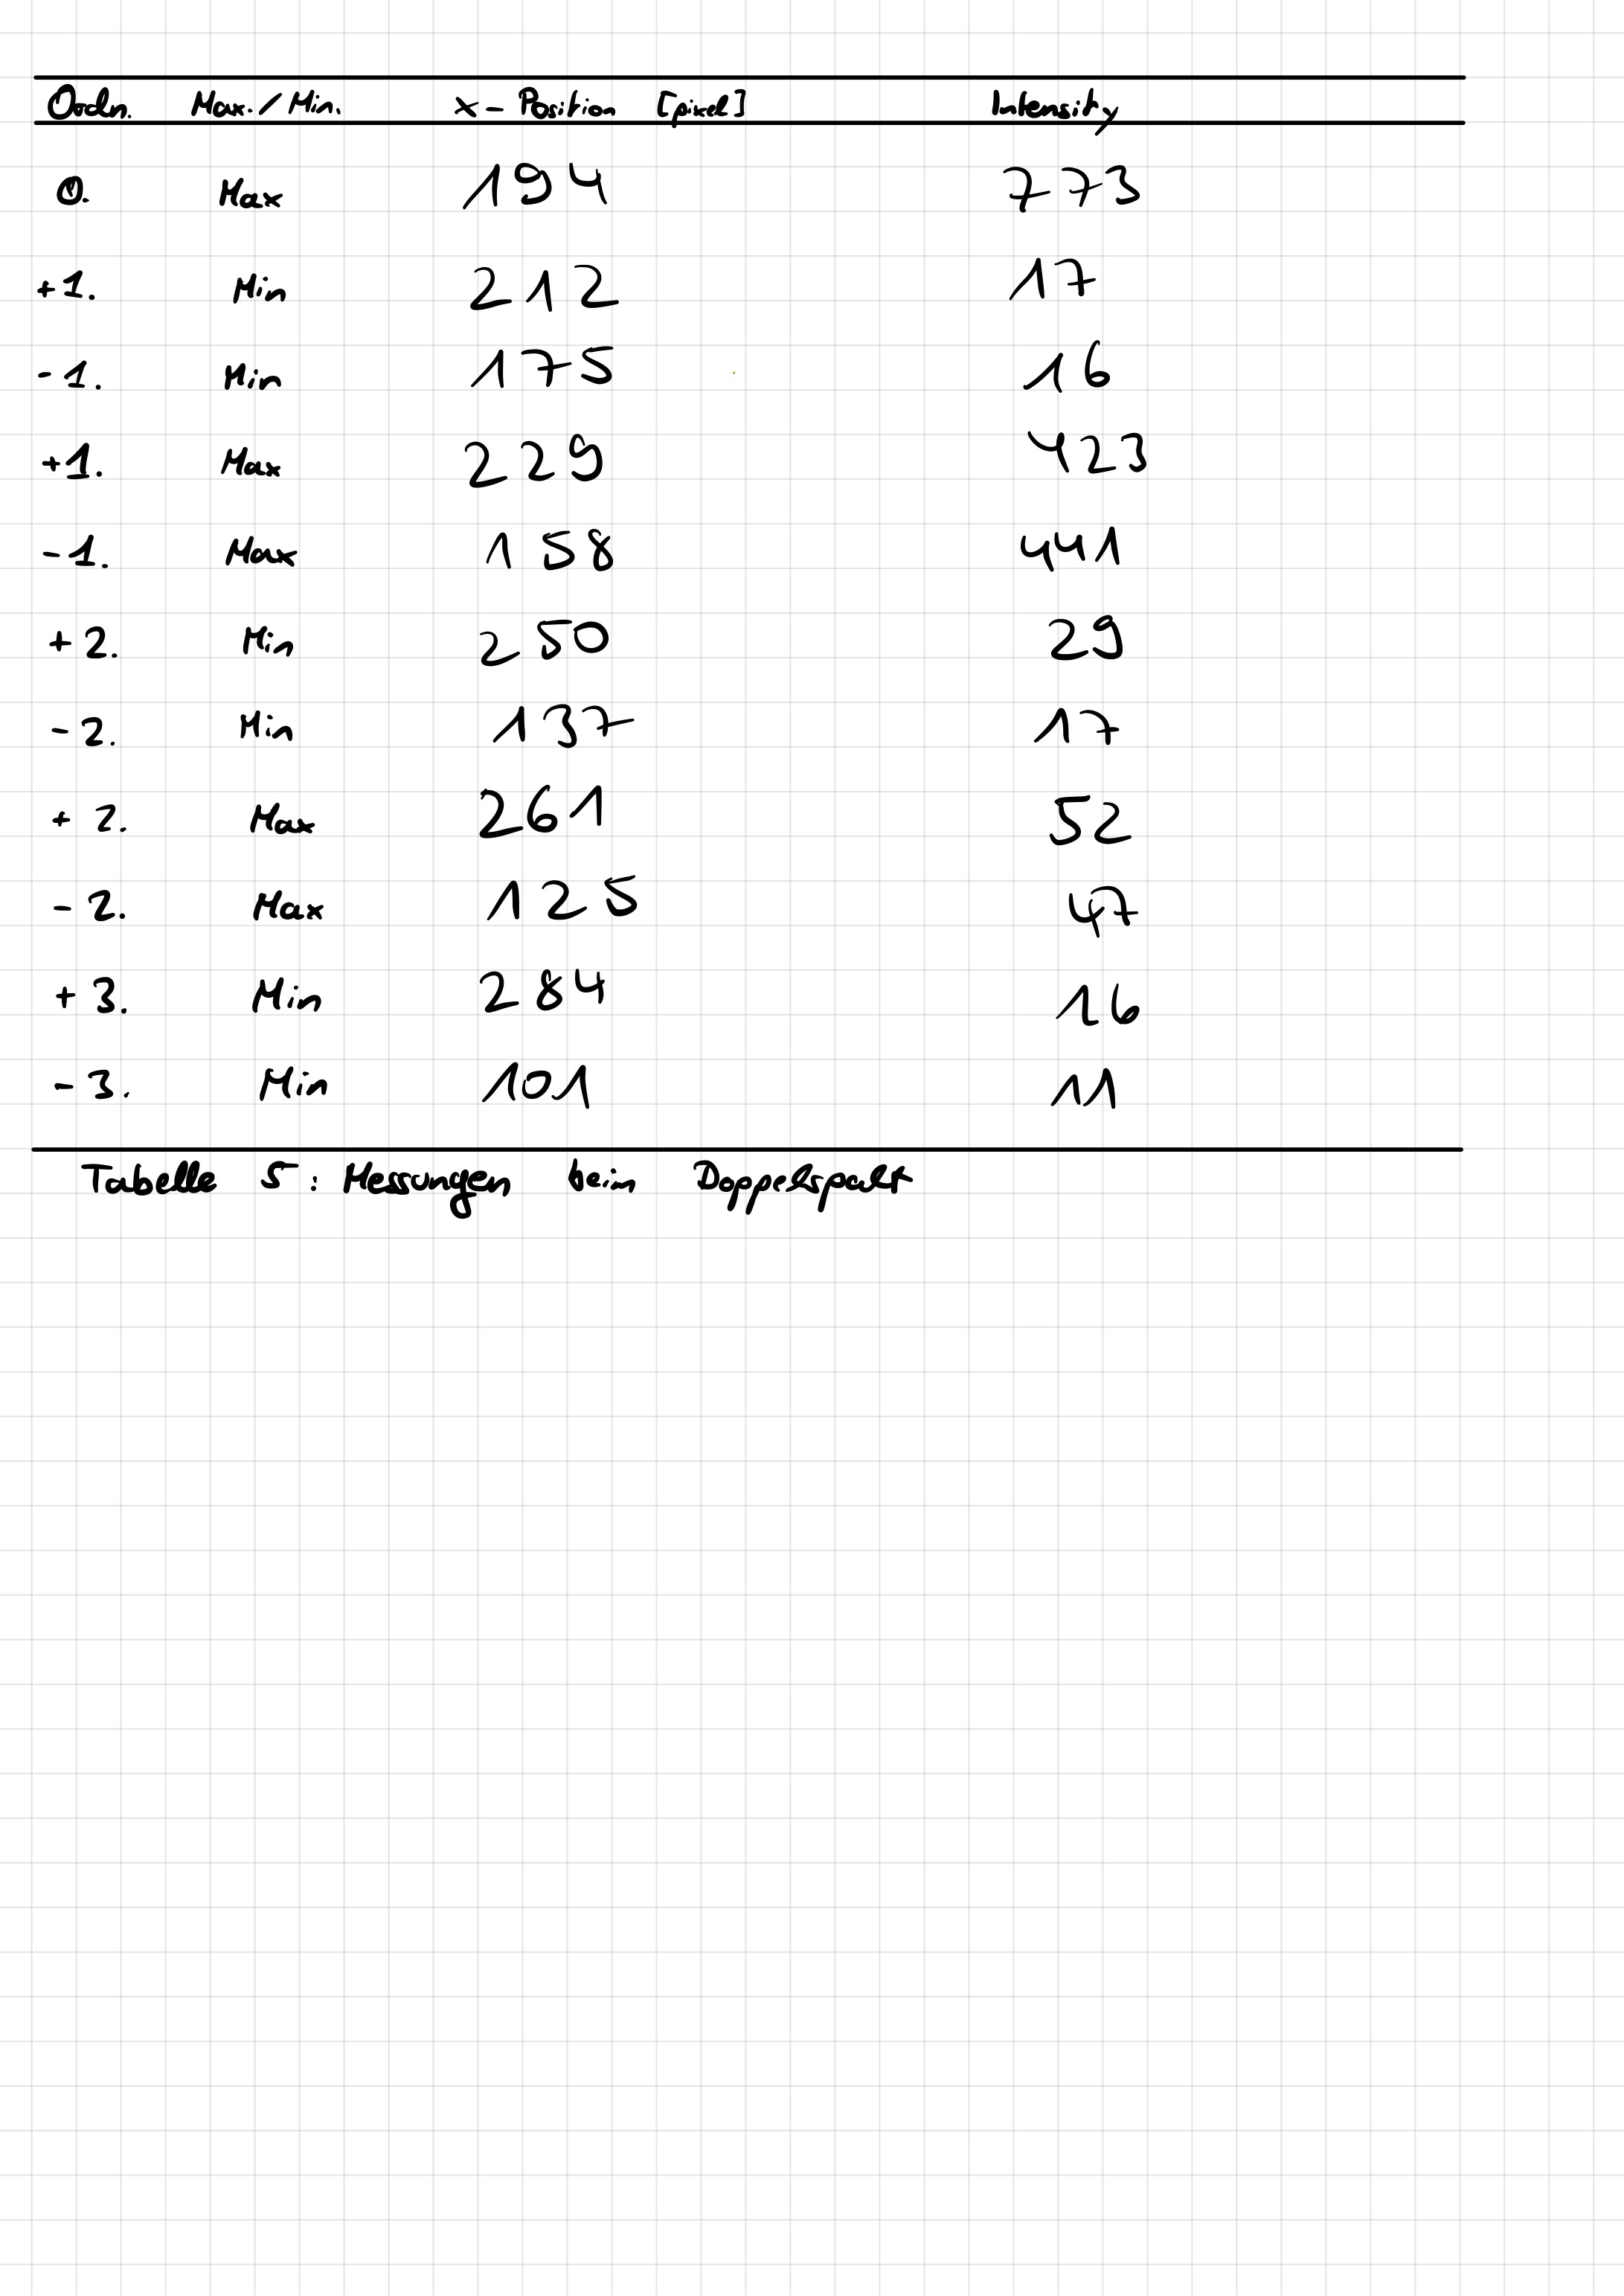
\includegraphics[width=\textwidth]{graphics/messprotokoll/233 - Fourieroptik-9.jpg}
\newpage
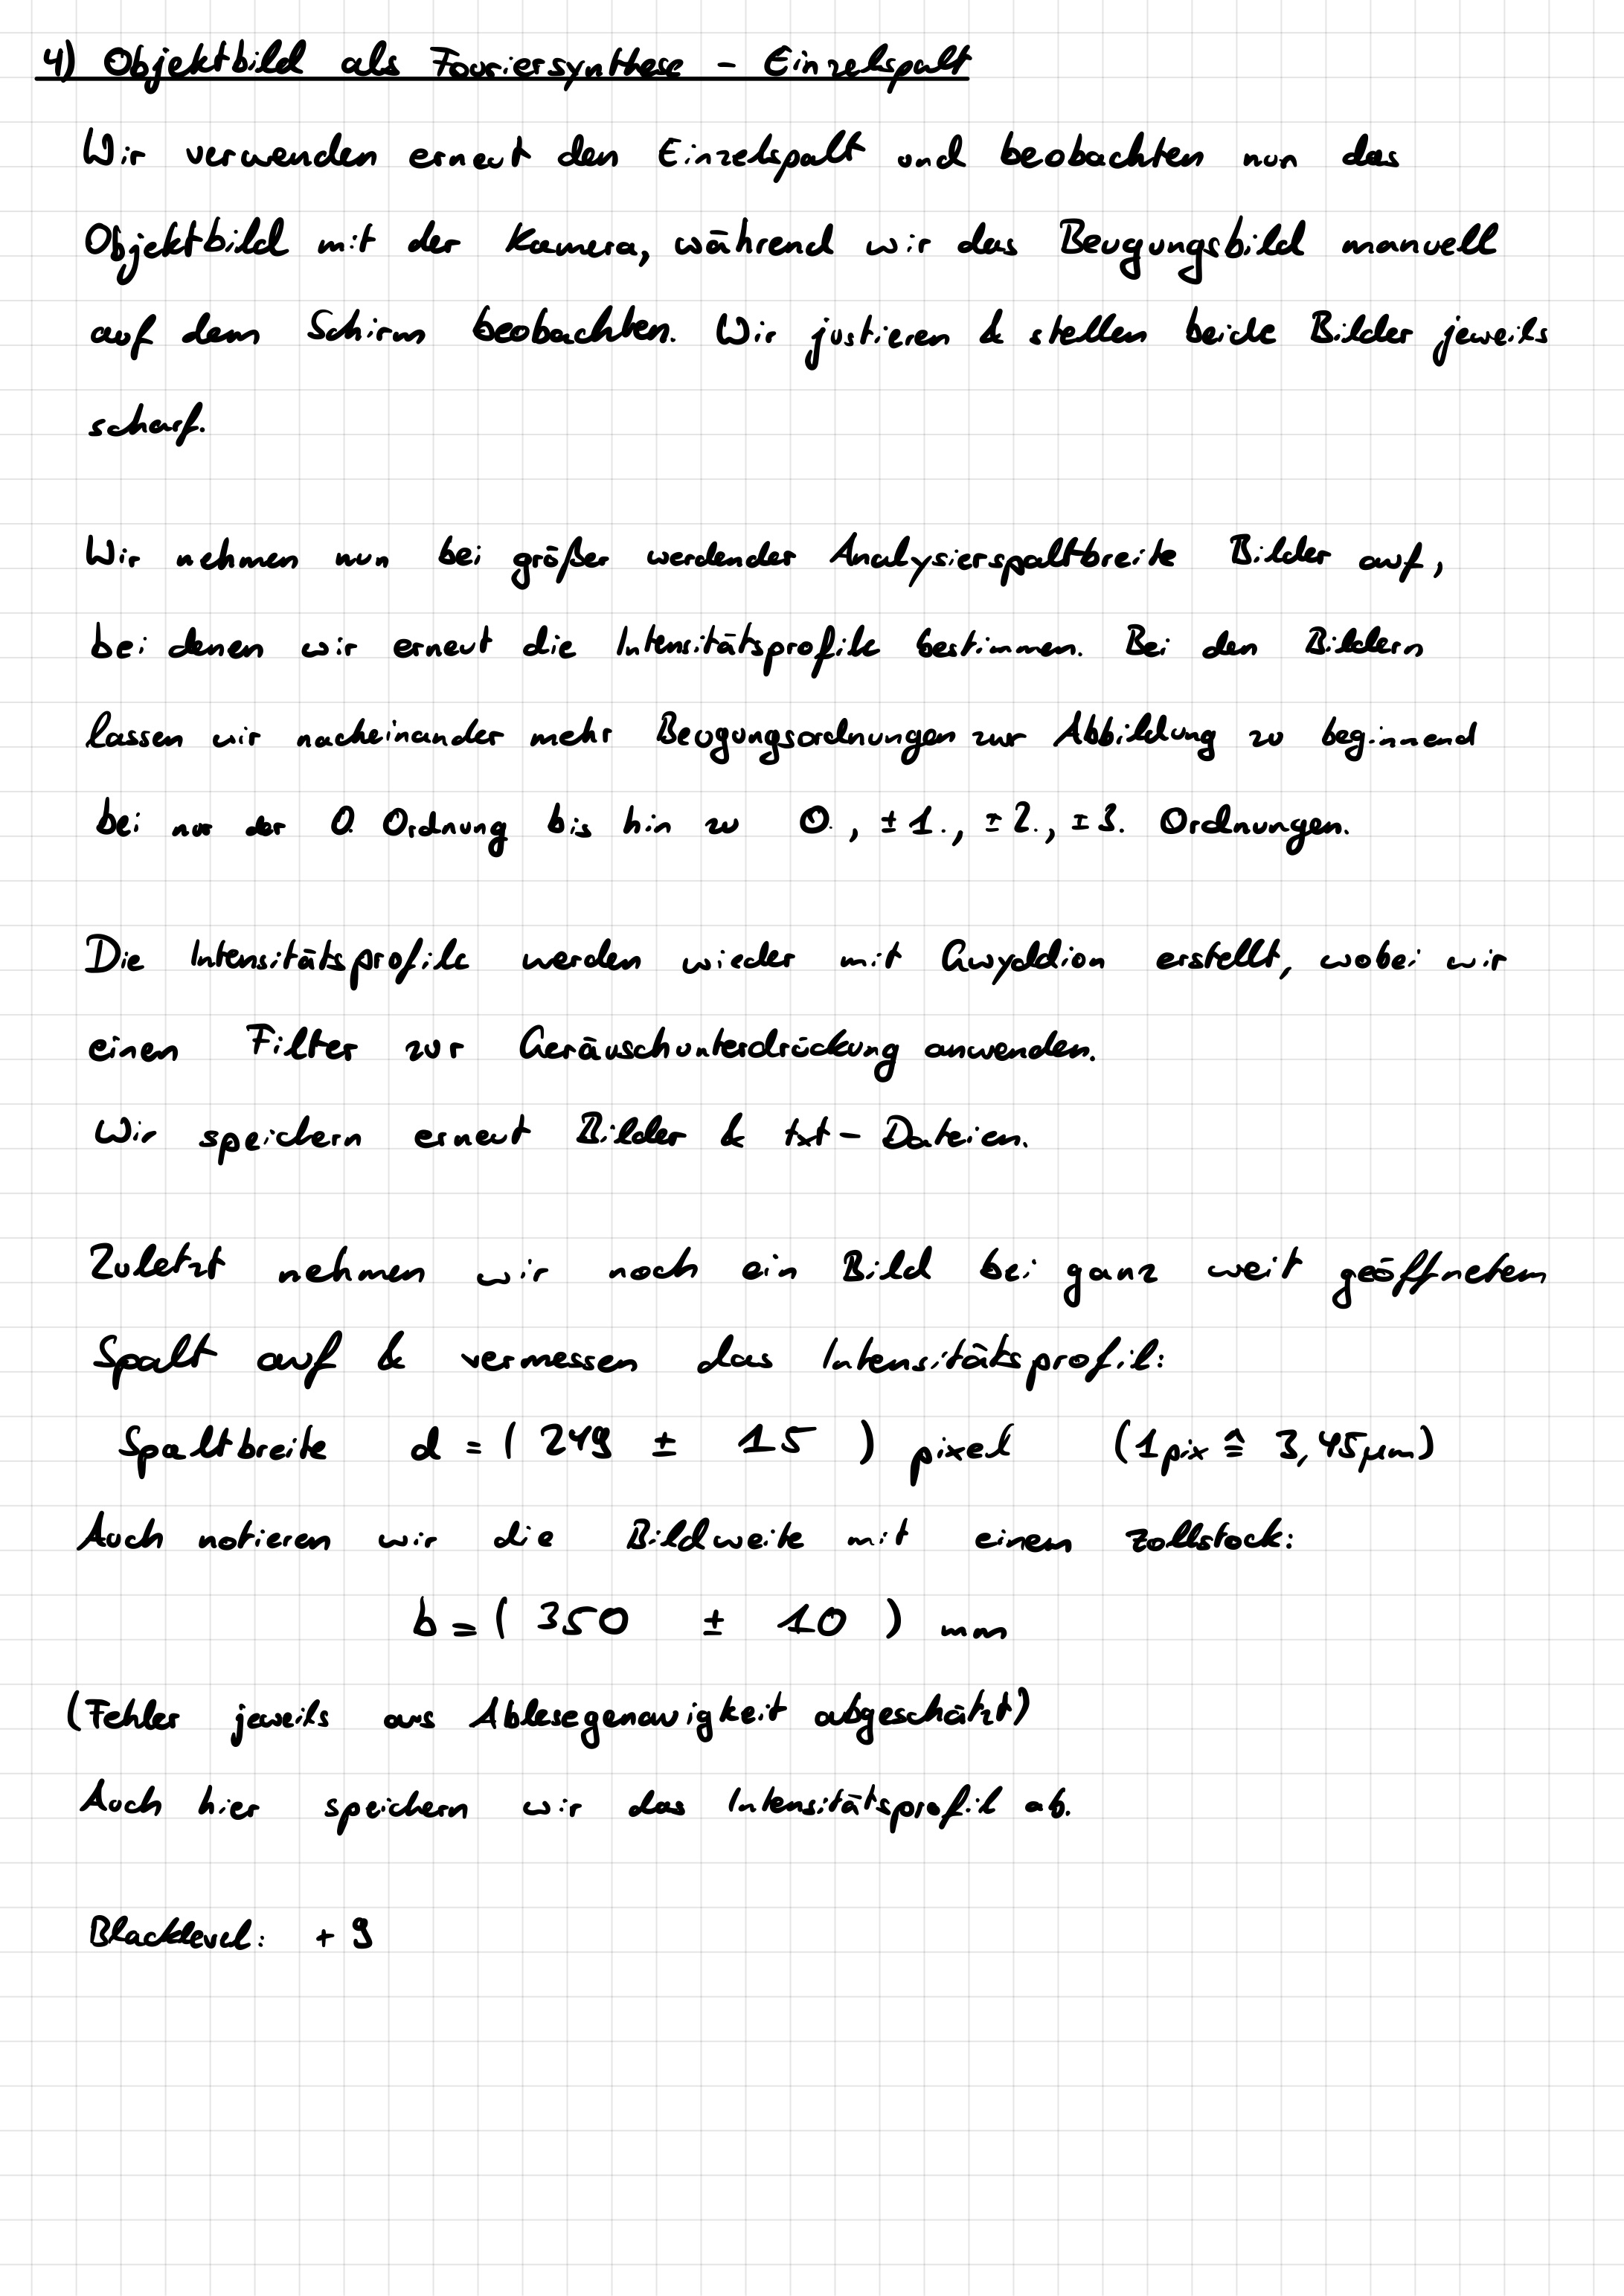
\includegraphics[width=\textwidth]{graphics/messprotokoll/233 - Fourieroptik-10.jpg}
\newpage
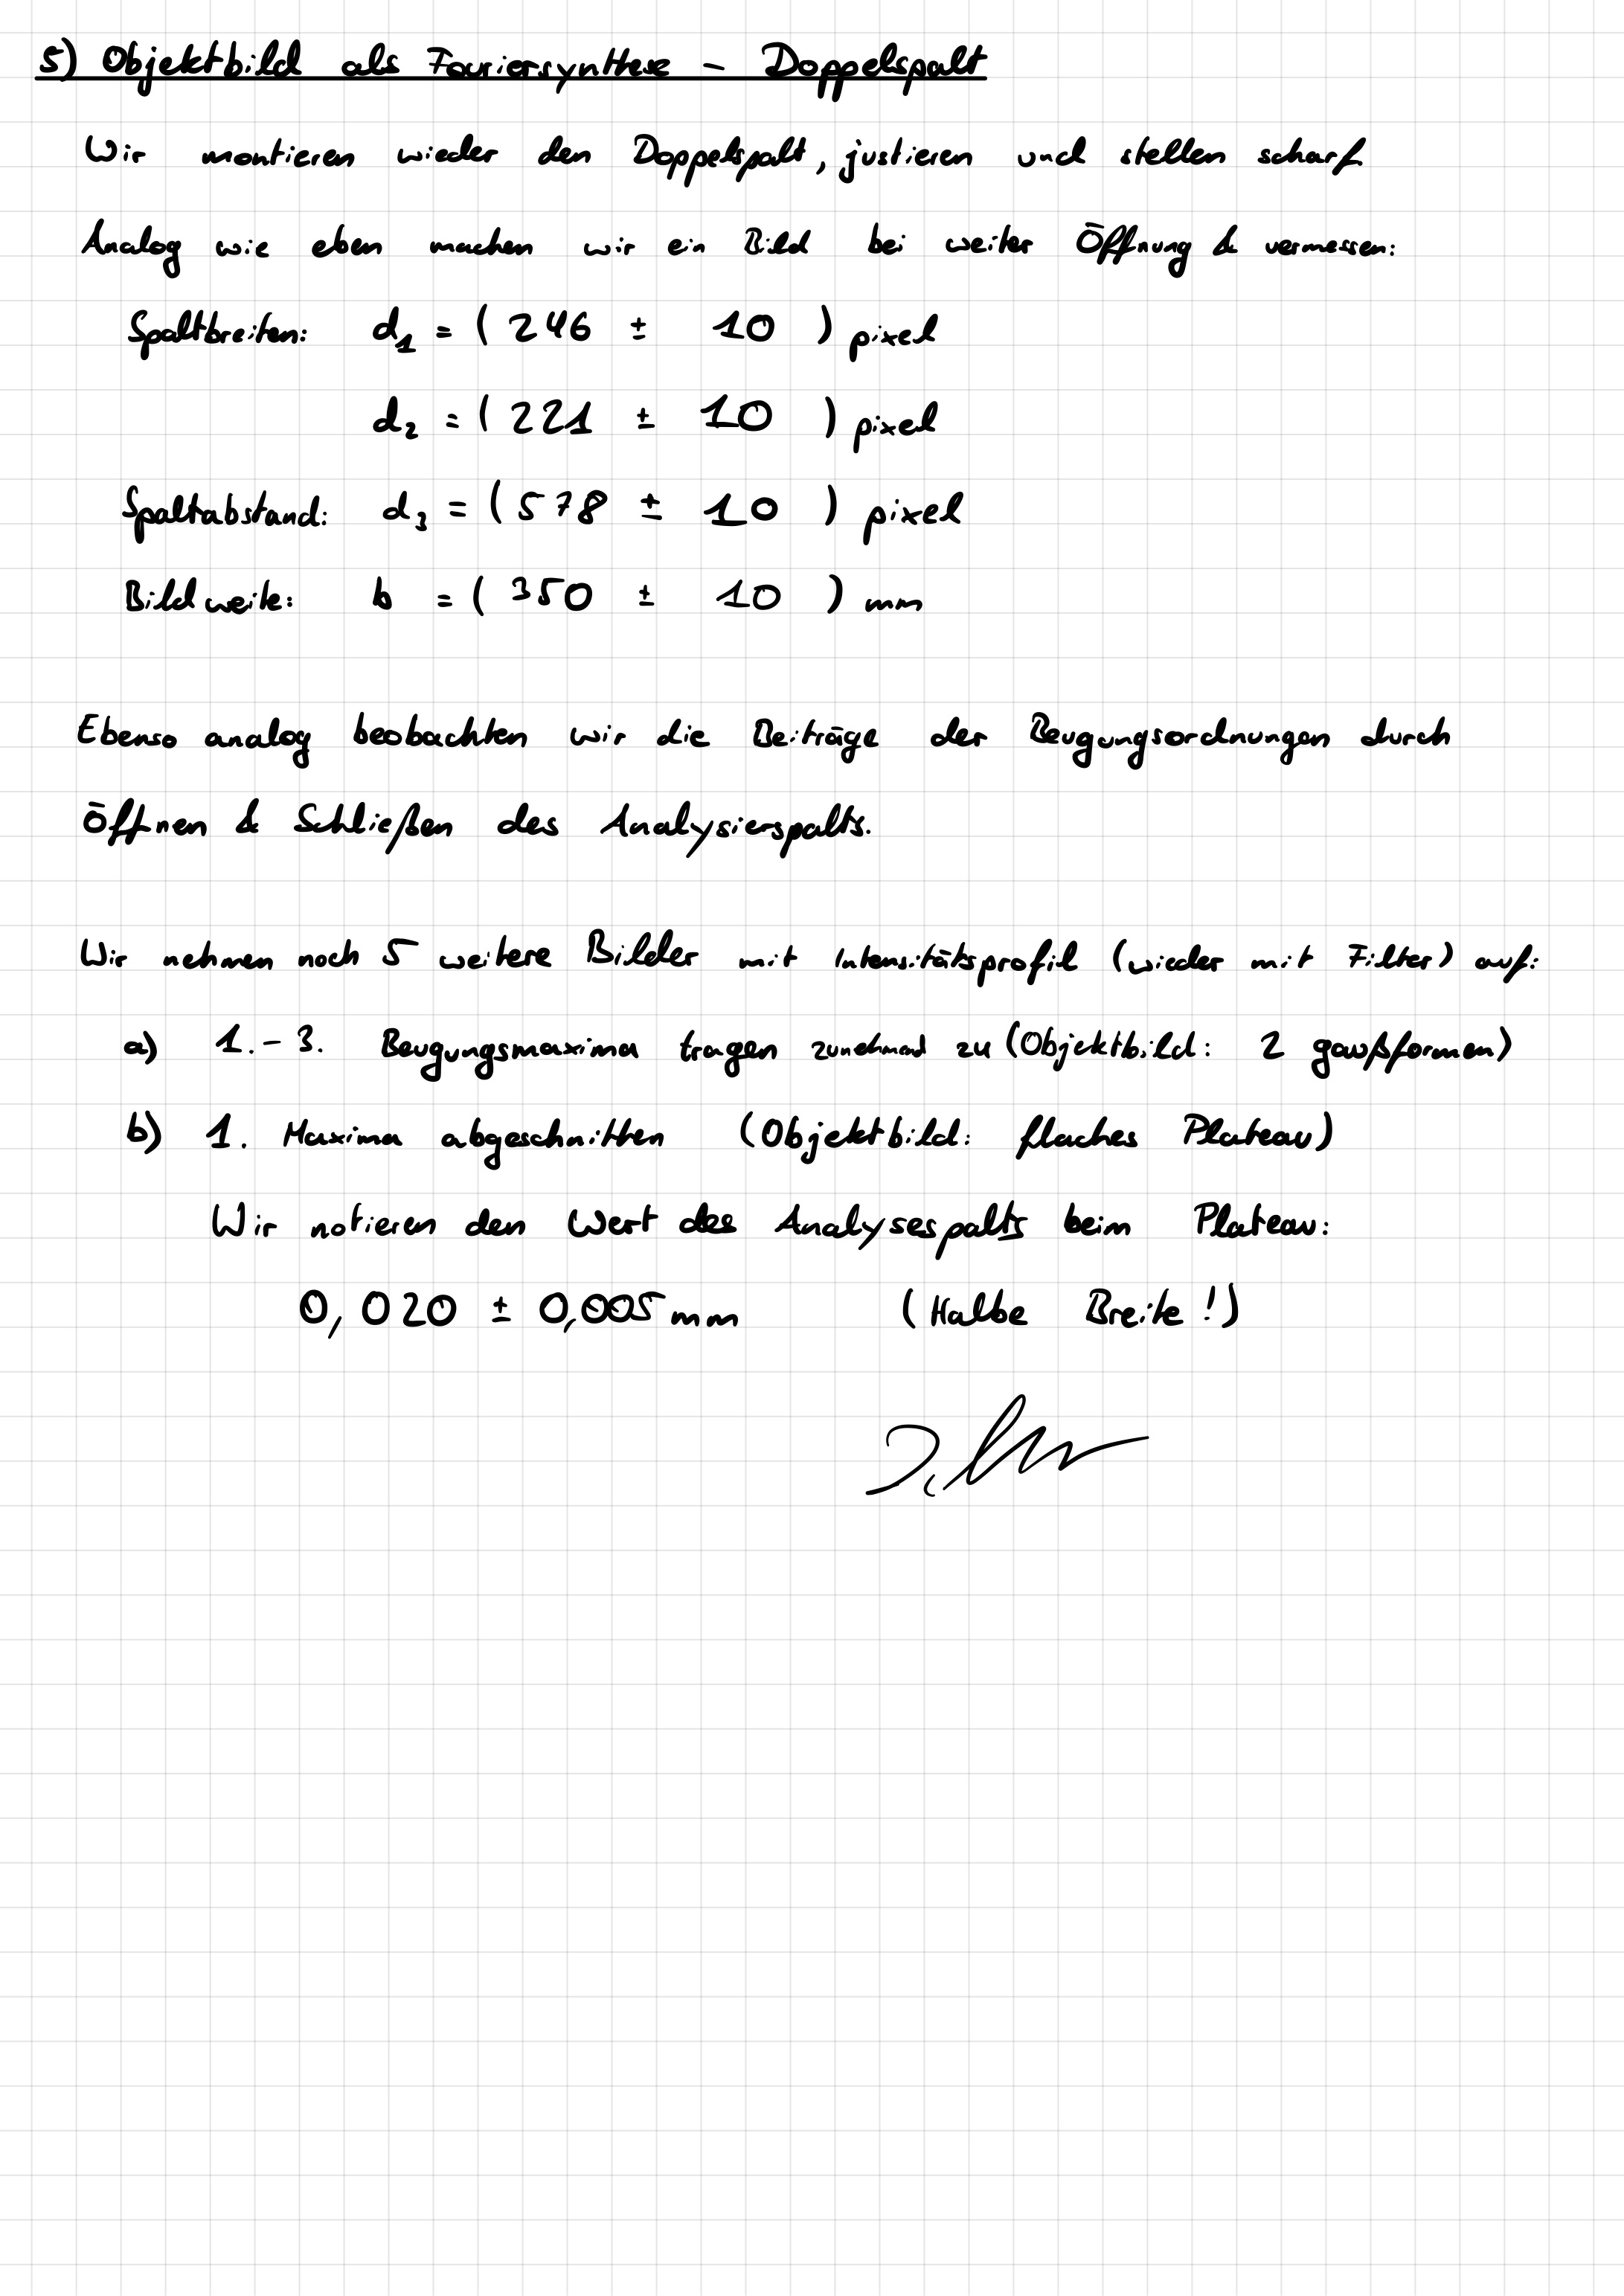
\includegraphics[width=\textwidth]{graphics/messprotokoll/233 - Fourieroptik-11.jpg}
\newpage

\addtocounter{table}{5}

\clearpage
\newpage

\begin{figure}[p]
  \centering
  \subfloat[Einzelspalt - Hauptmaximum nicht in Sättigung]{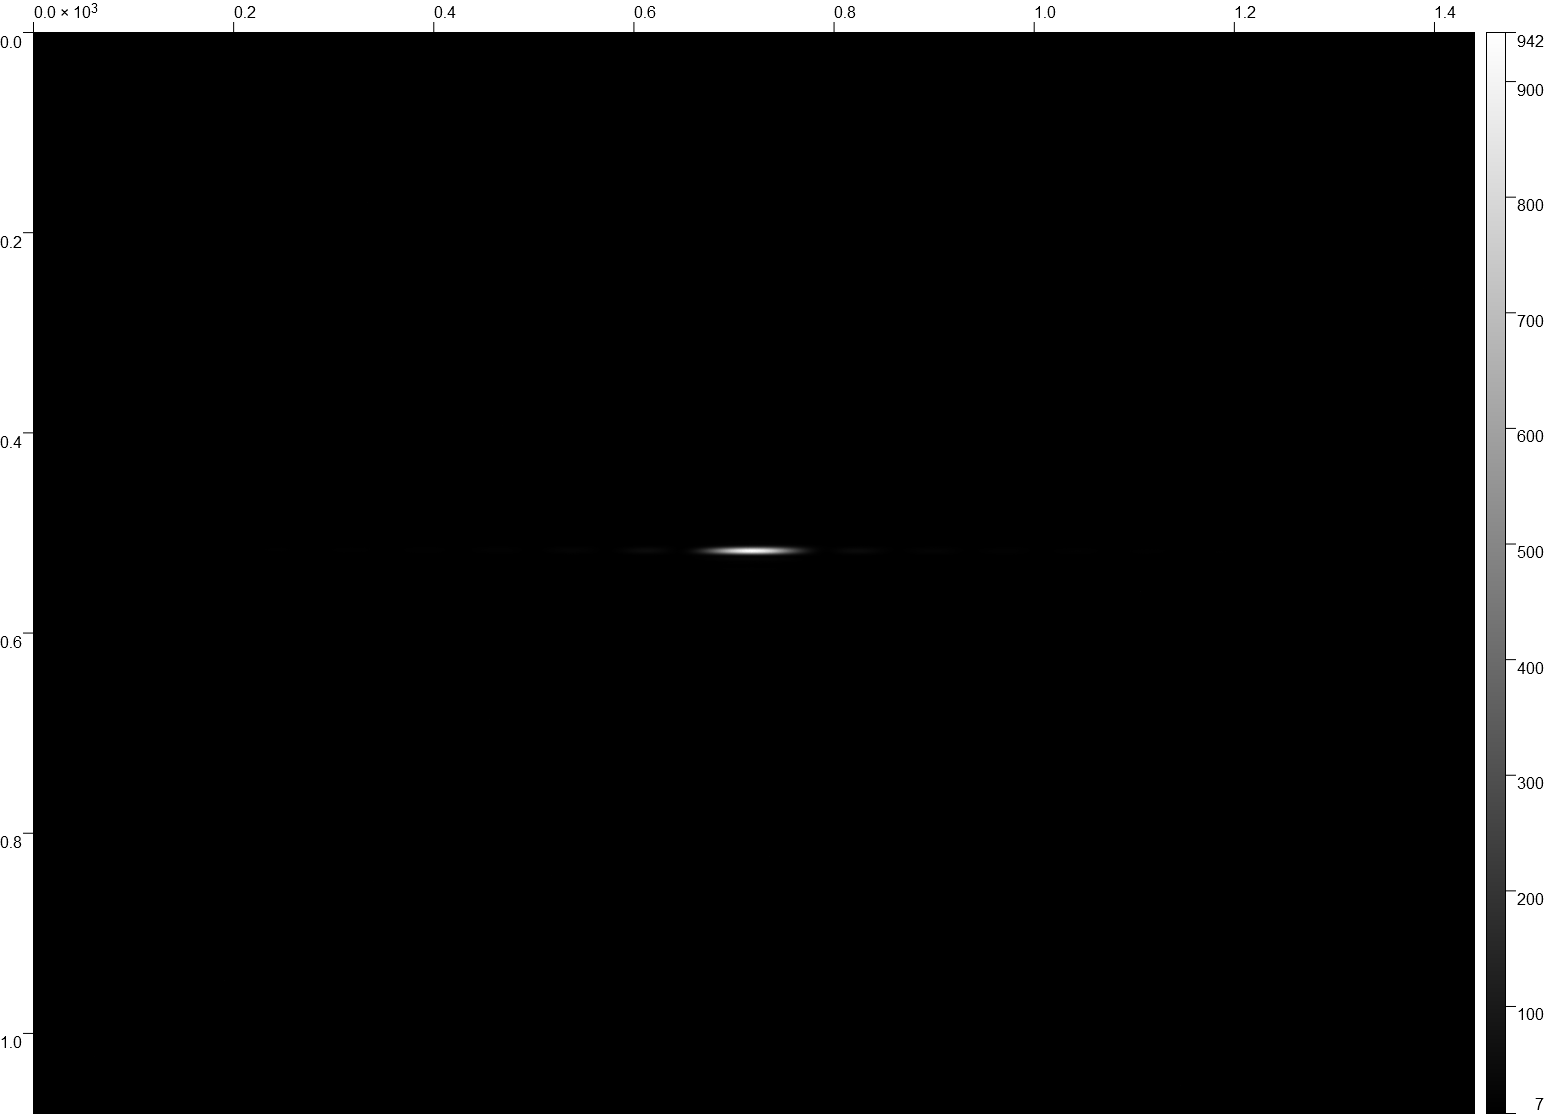
\includegraphics[width=0.65\textwidth]{graphics/aufnahmen/0_1_2024-03-12T09-57-57.186.png}}
  \hfill
  \subfloat[Einzelspalt - Hauptmaximum in Sättigung]{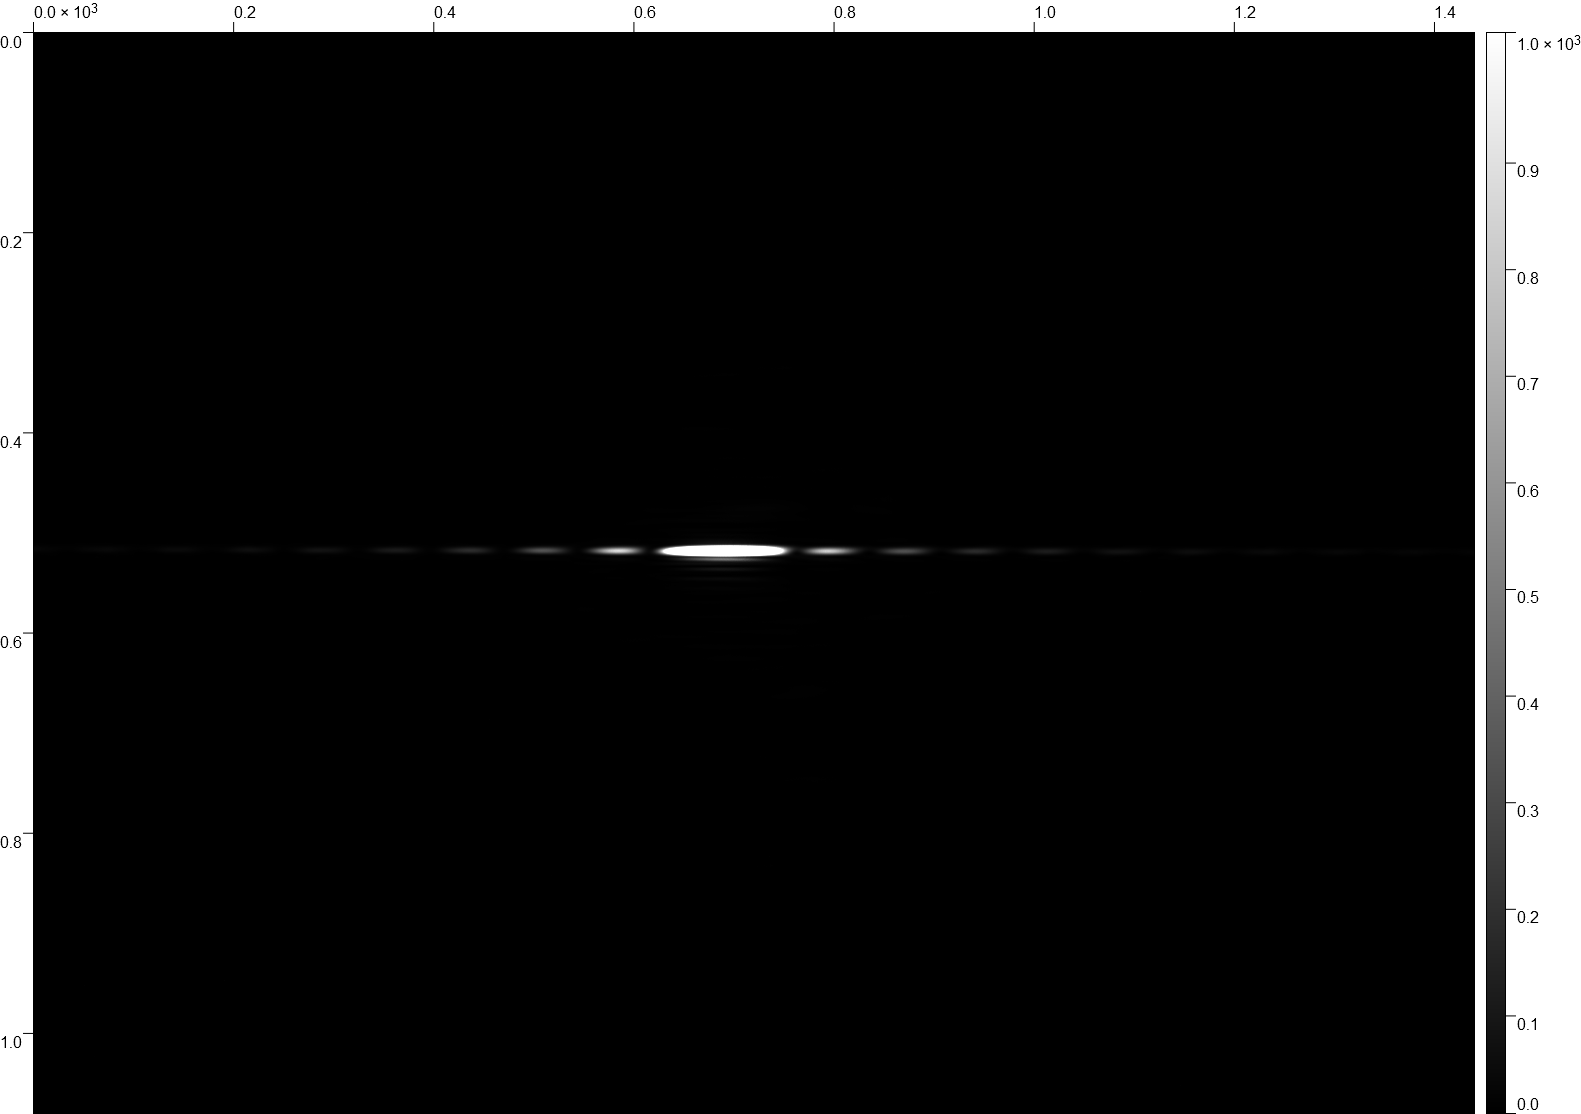
\includegraphics[width=0.65\textwidth]{graphics/aufnahmen/0_1_2_3_4_2024-03-12T10-11-50.899.png}}
  \hfill
  \subfloat[Doppelspalt]{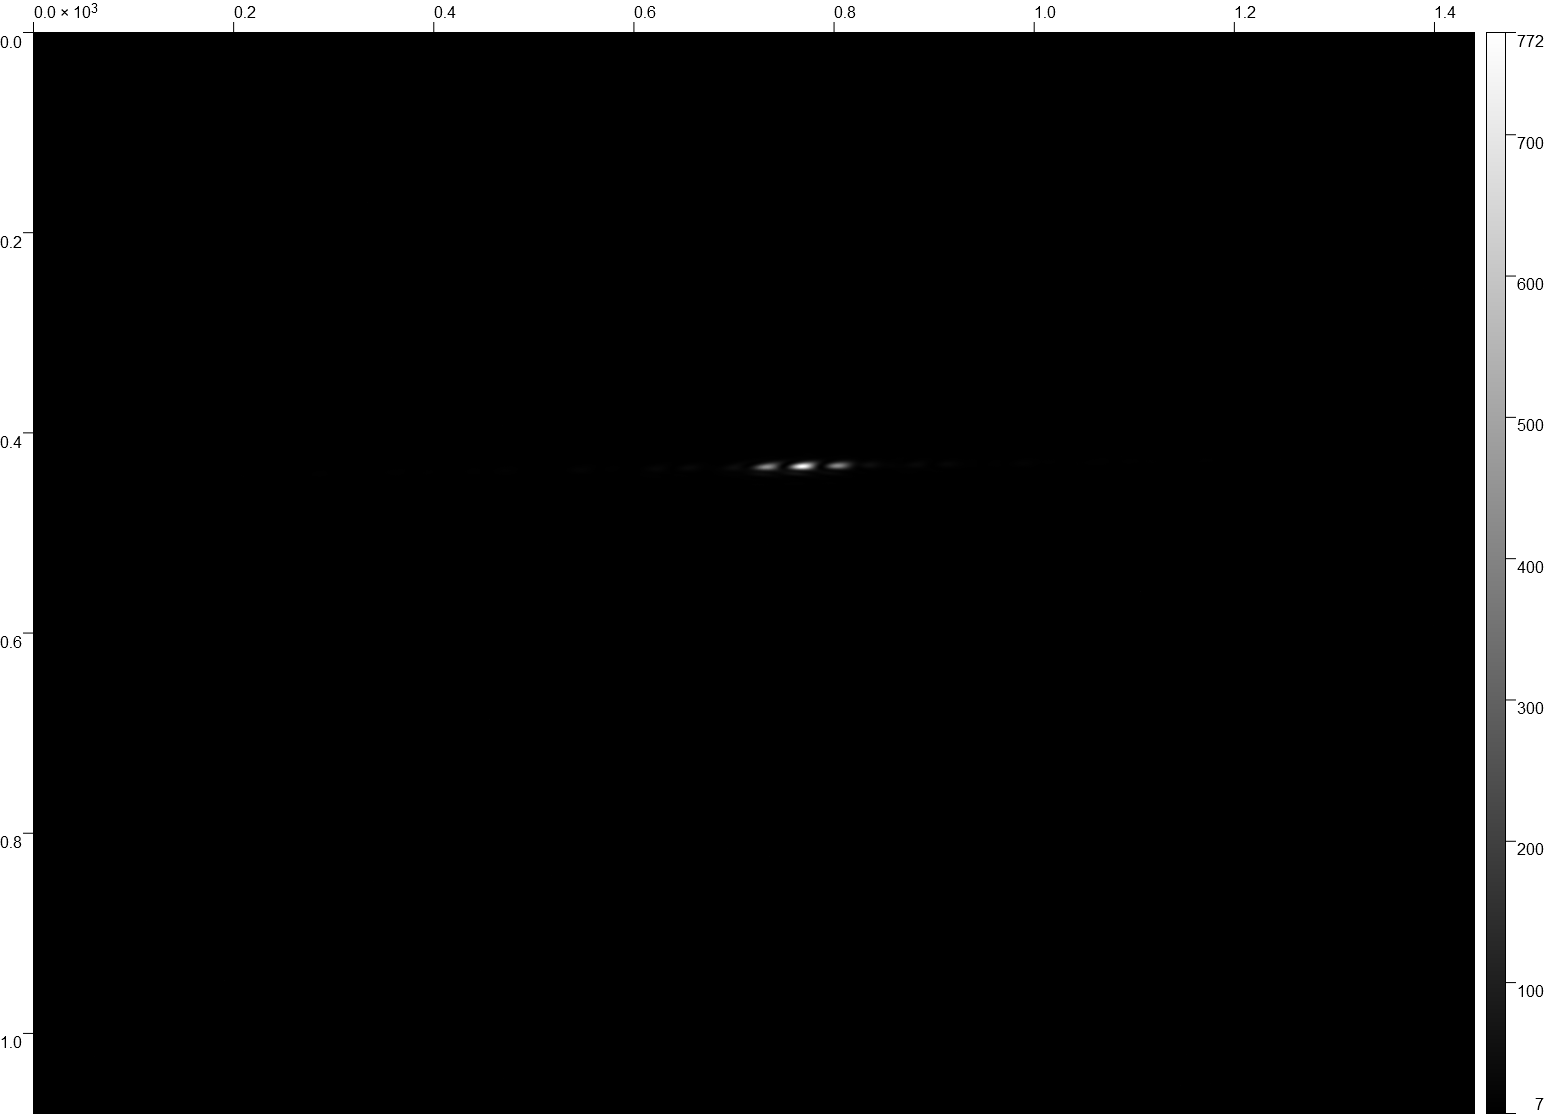
\includegraphics[width=0.65\textwidth]{graphics/aufnahmen/doppelspalt_2024-03-12T11-02-30.5.png}}
  \hfill
  \caption{Aufgenommene Beugungsbilder}
  \label{fig:Aufnahmen_Beugungsbilder}
\end{figure}

\clearpage
\newpage

\begin{figure}[p]
  \centering
  \subfloat[nur 0. Beugungsmaximum]{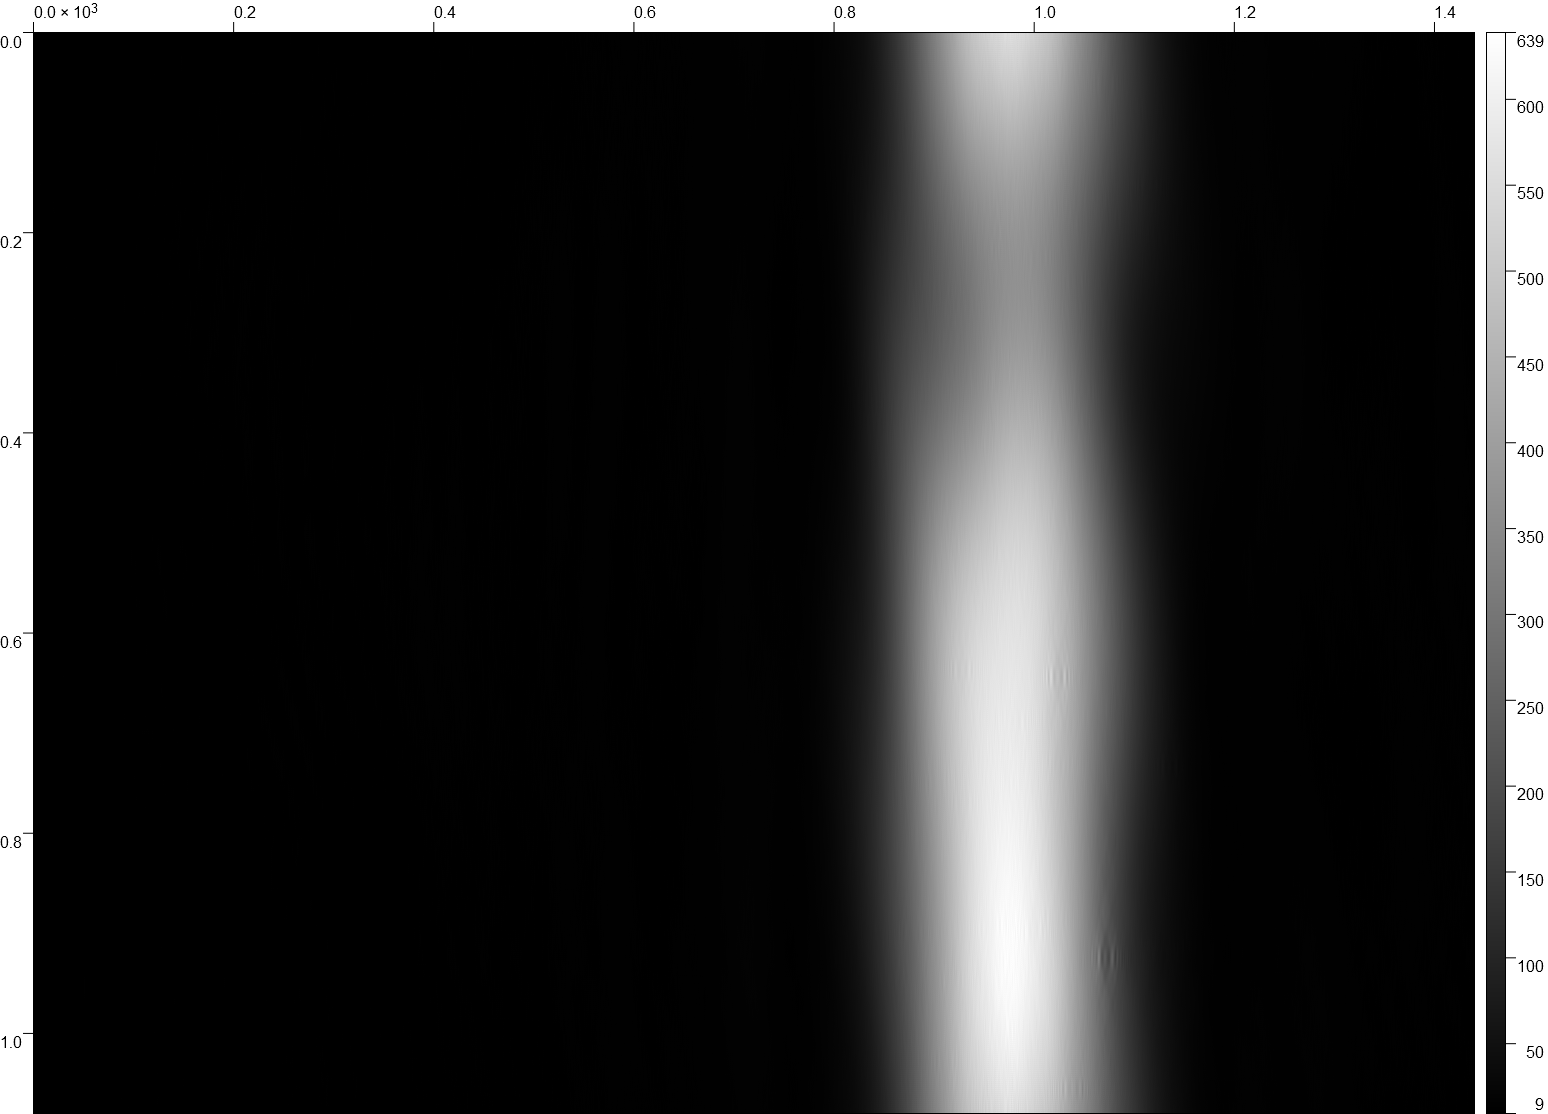
\includegraphics[width=0.48\textwidth]{graphics/aufnahmen/objektbild_einzelspalt_0_2024-03-14T10-32-51.979_clean.png}}
  \hfill
  \subfloat[0. + 1. Beugungsmaximum]{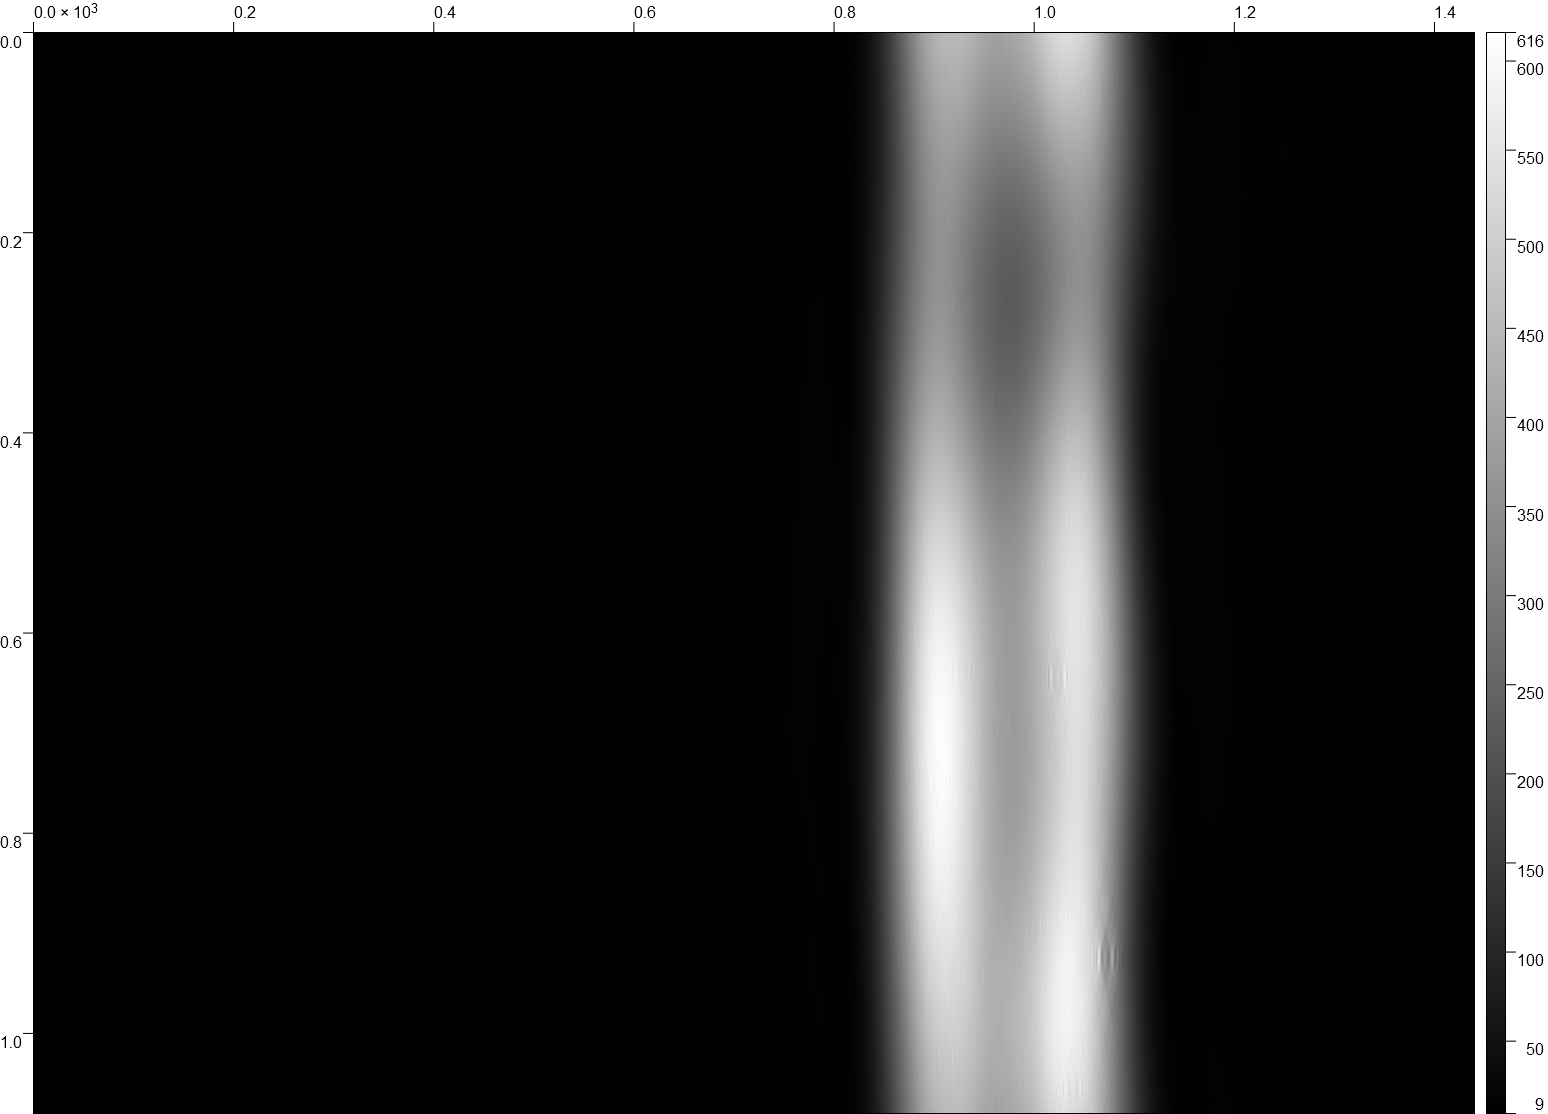
\includegraphics[width=0.48\textwidth]{graphics/aufnahmen/objektbild_einzelspalt_0+1_2024-03-14T10-32-26.371_clean.png}}
  \hfill
  \subfloat[0. - 2. Beugungsmaximum]{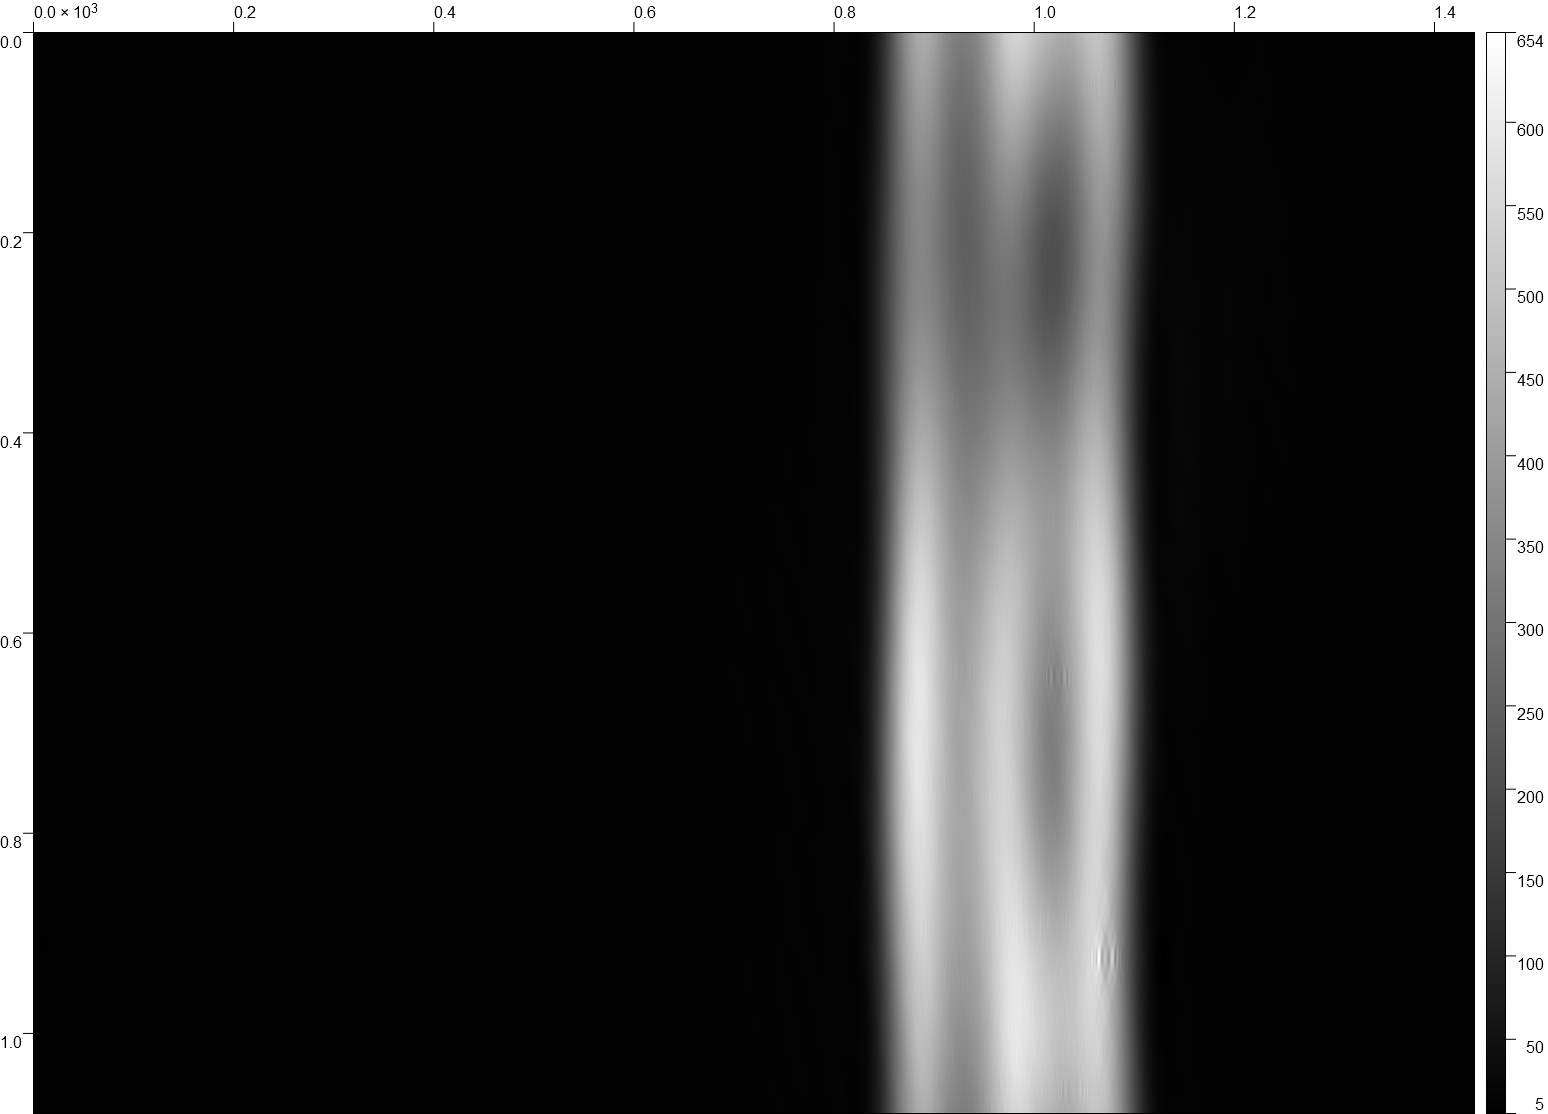
\includegraphics[width=0.48\textwidth]{graphics/aufnahmen/objektbild_einzelspalt_0+1+2_2024-03-14T10-33-26.692_clean.png}}
  \hfill
  \subfloat[0. - 3. Beugungsmaximum]{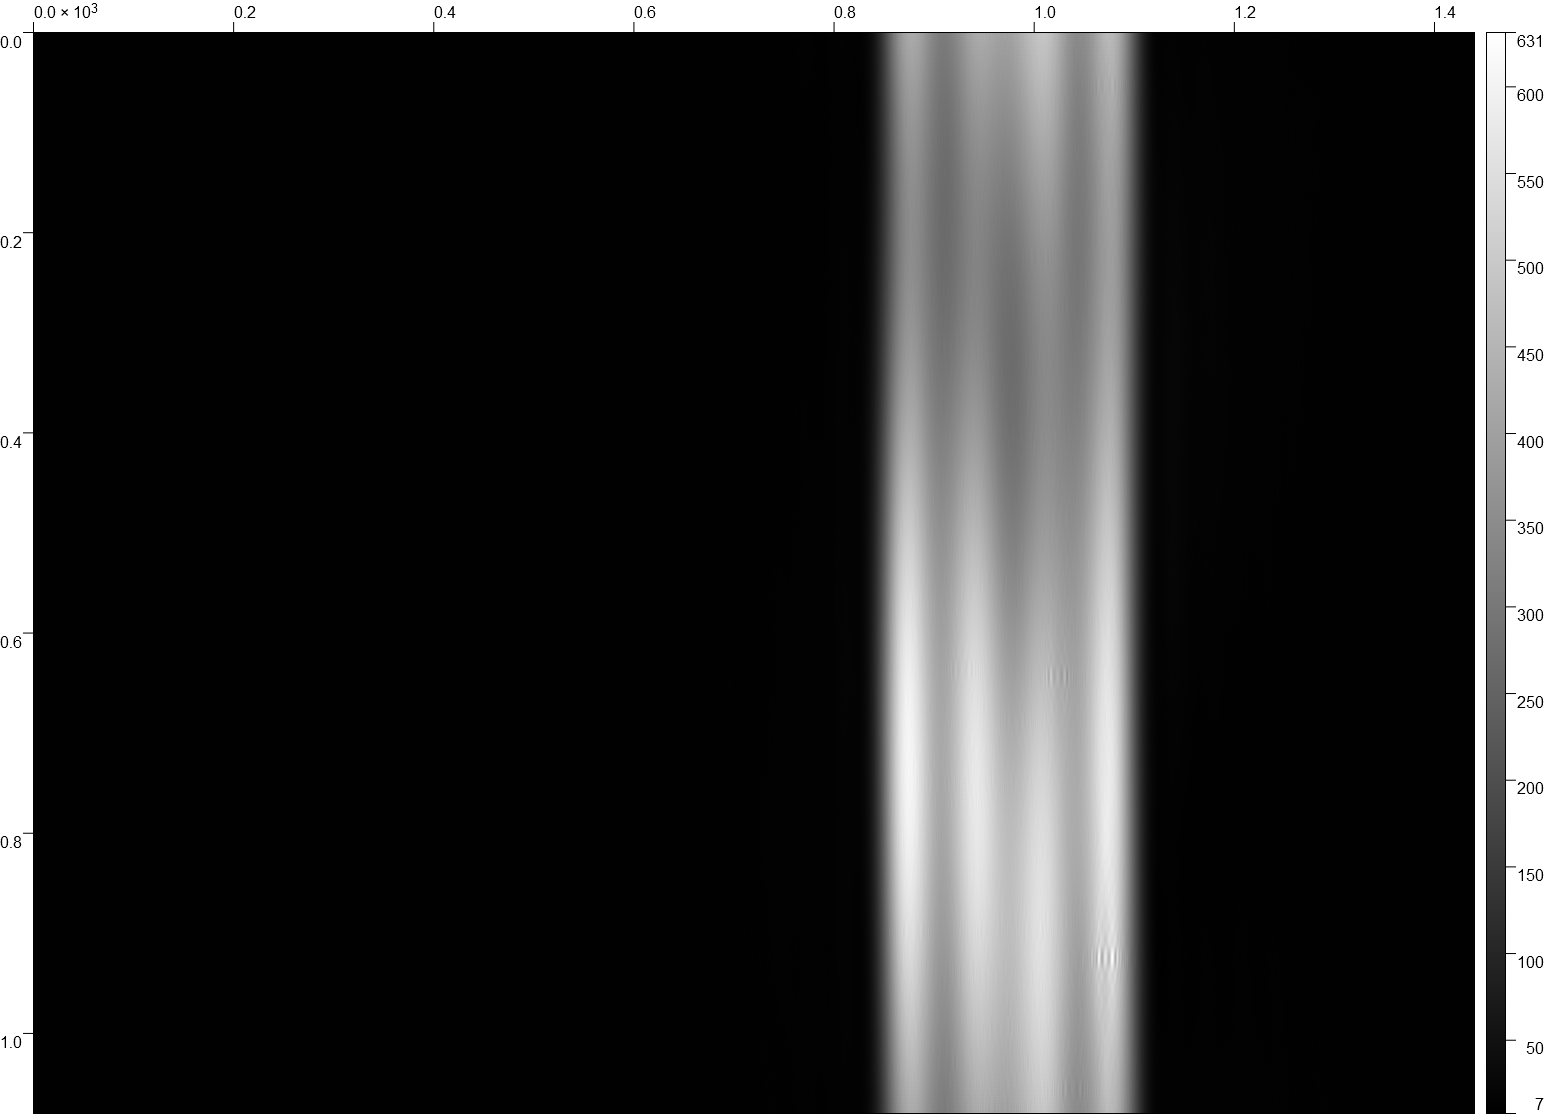
\includegraphics[width=0.48\textwidth]{graphics/aufnahmen/objektbild_einzelspalt_0+1+2+3_2024-03-14T10-34-04.883_clean.png}}
  \hfill
  \subfloat[alle Beugungsmaxima]{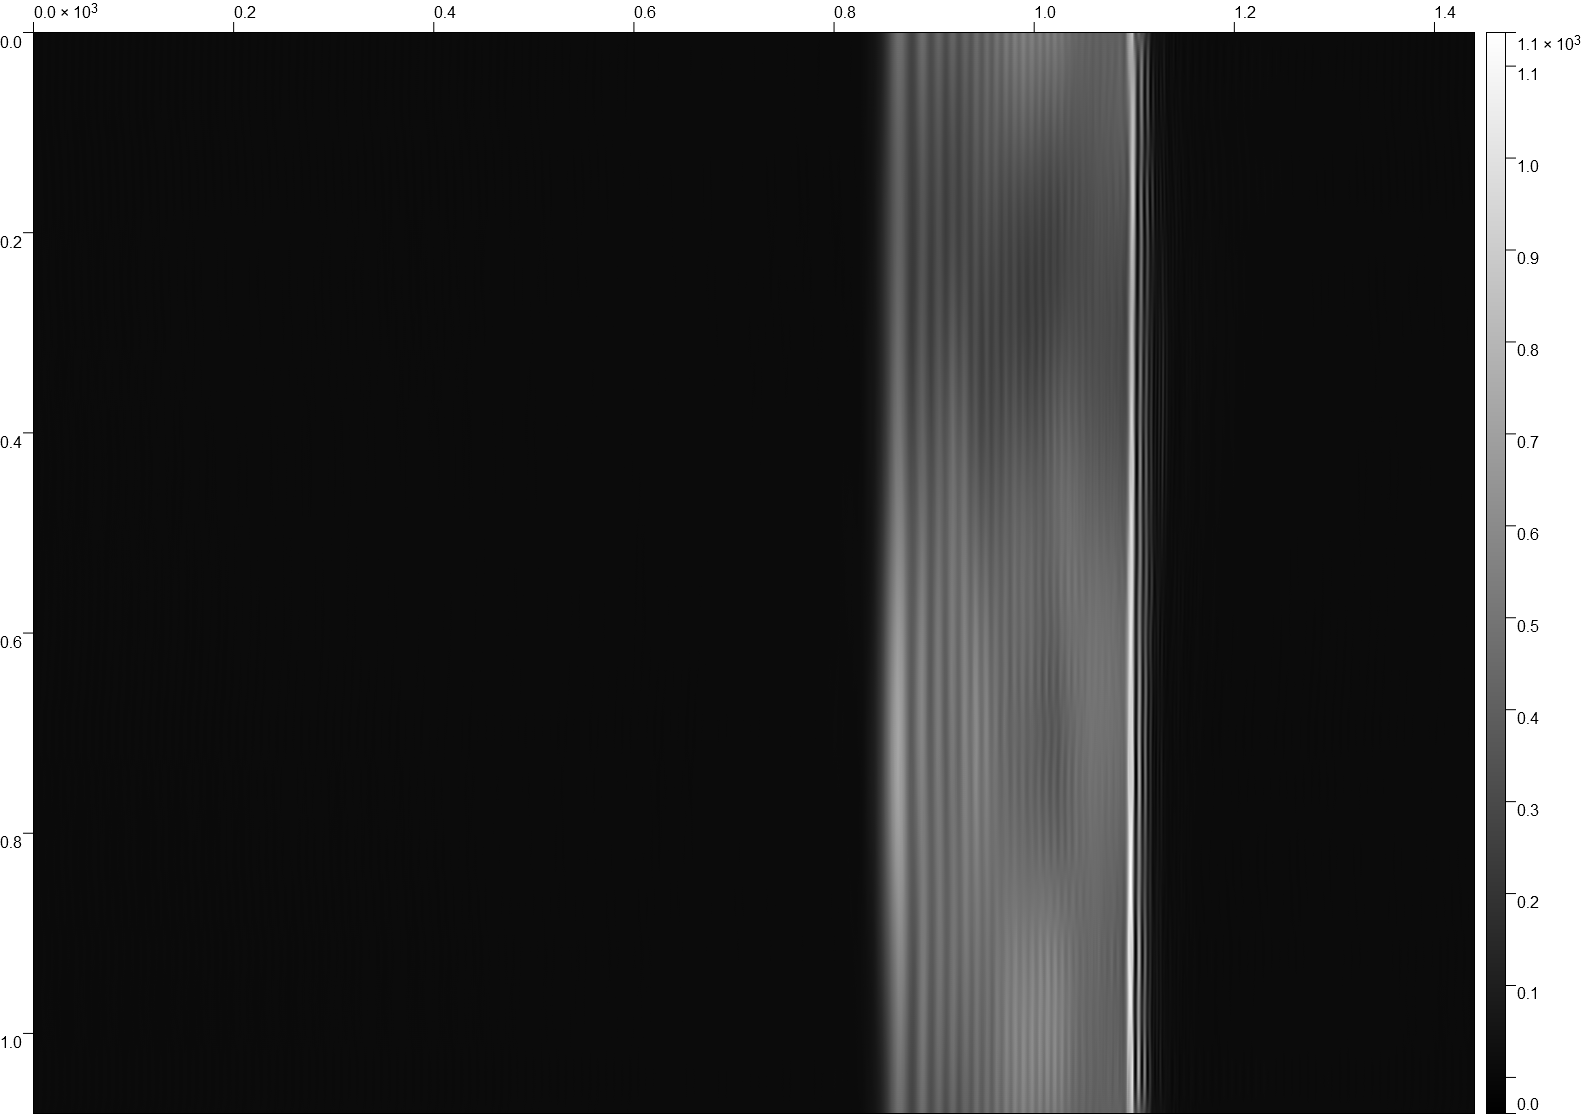
\includegraphics[width=0.48\textwidth]{graphics/aufnahmen/objektbild_einzelspalt_full_2024-03-14T10-52-12.146_clean.png}}
  \hfill
  \caption{Aufgenommene Objektbilder - Einzel}
  \label{fig:Aufnahmen_Obj_Einzel}
\end{figure}

\clearpage
\newpage

\begin{figure}[p]
  \centering
  \subfloat[nur 0. Beugungsmaximum]{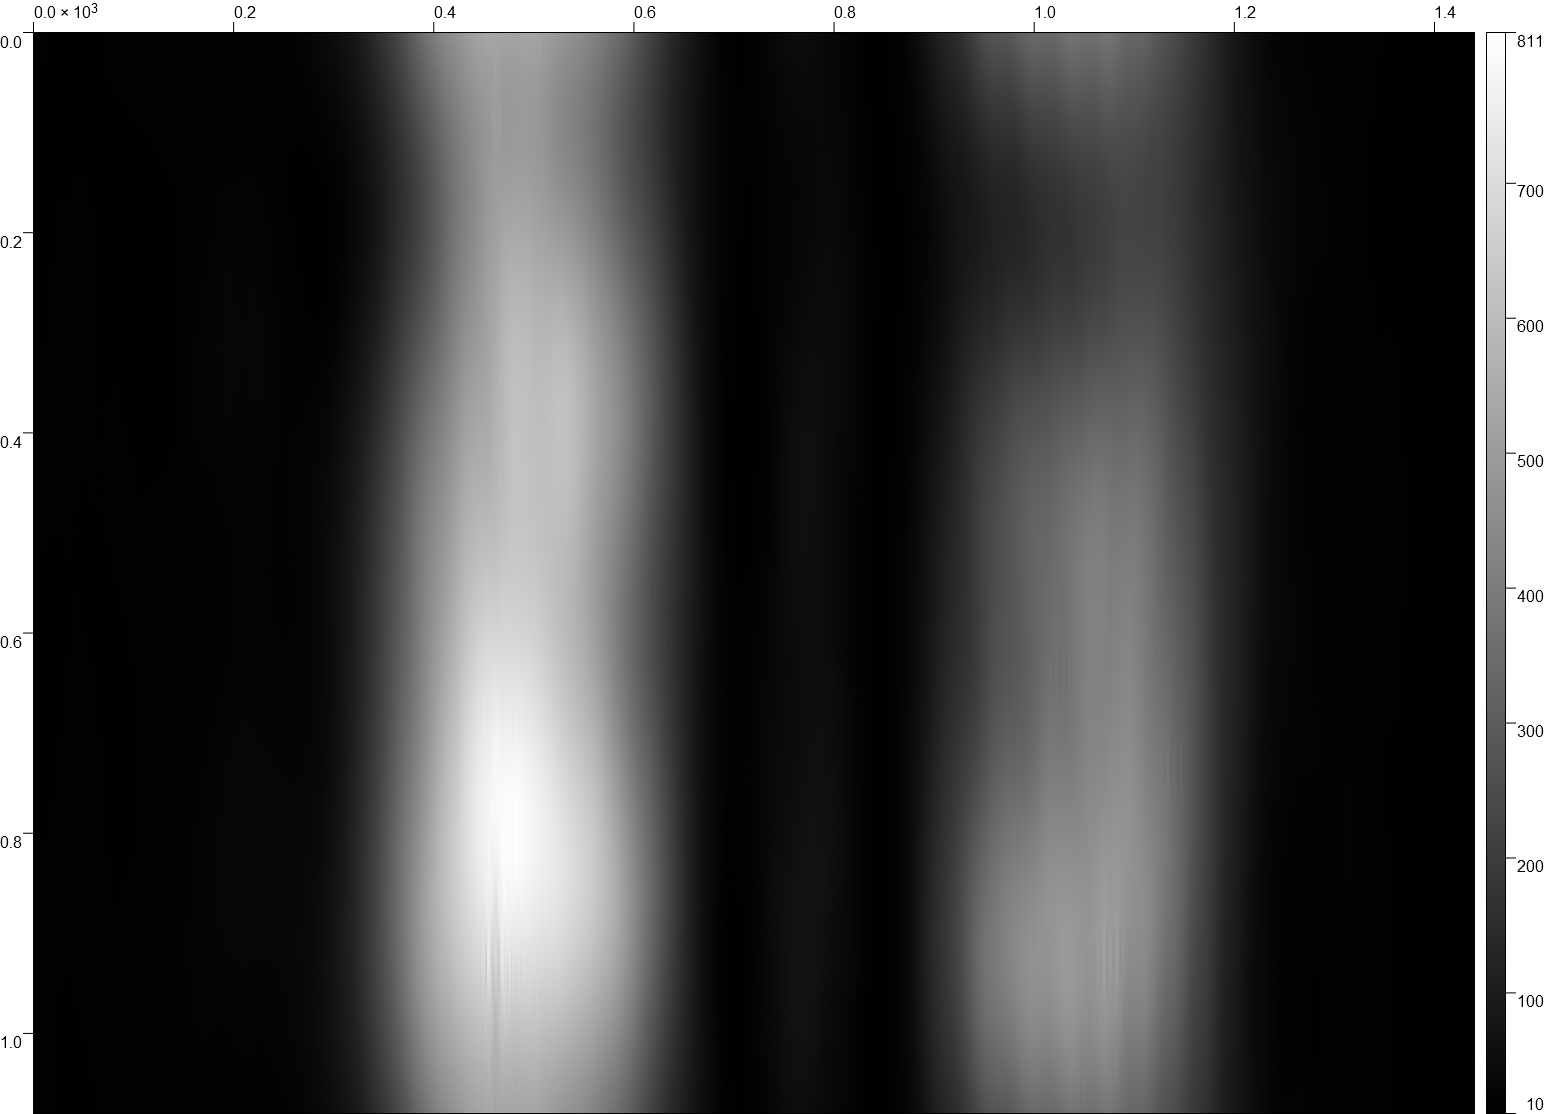
\includegraphics[width=0.48\textwidth]{graphics/aufnahmen/objektbild_doppelspalt_0_2024-03-14T11-39-55.236_clear.png}}
  \hfill
  \subfloat[0. + 1. Beugungsmaximum]{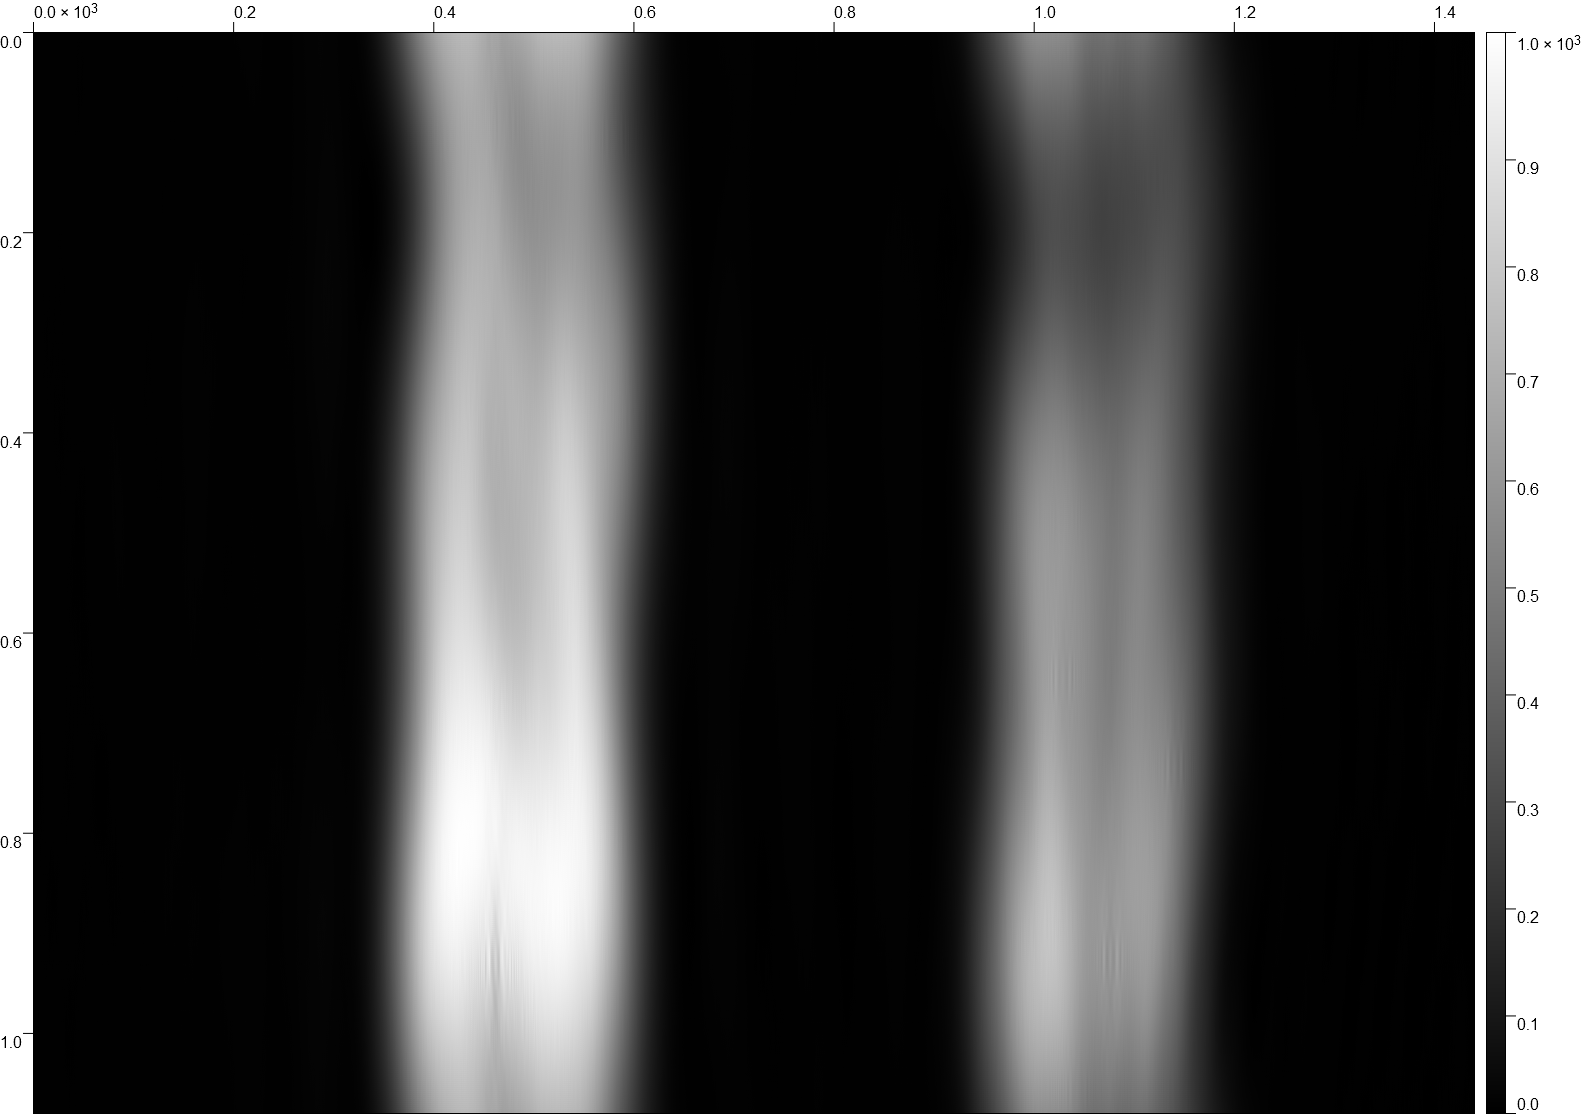
\includegraphics[width=0.48\textwidth]{graphics/aufnahmen/objektbild_doppelspalt_0_1_2024-03-14T11-40-49.132_clear.png}}
  \hfill
  \subfloat[0. - 2. Beugungsmaximum]{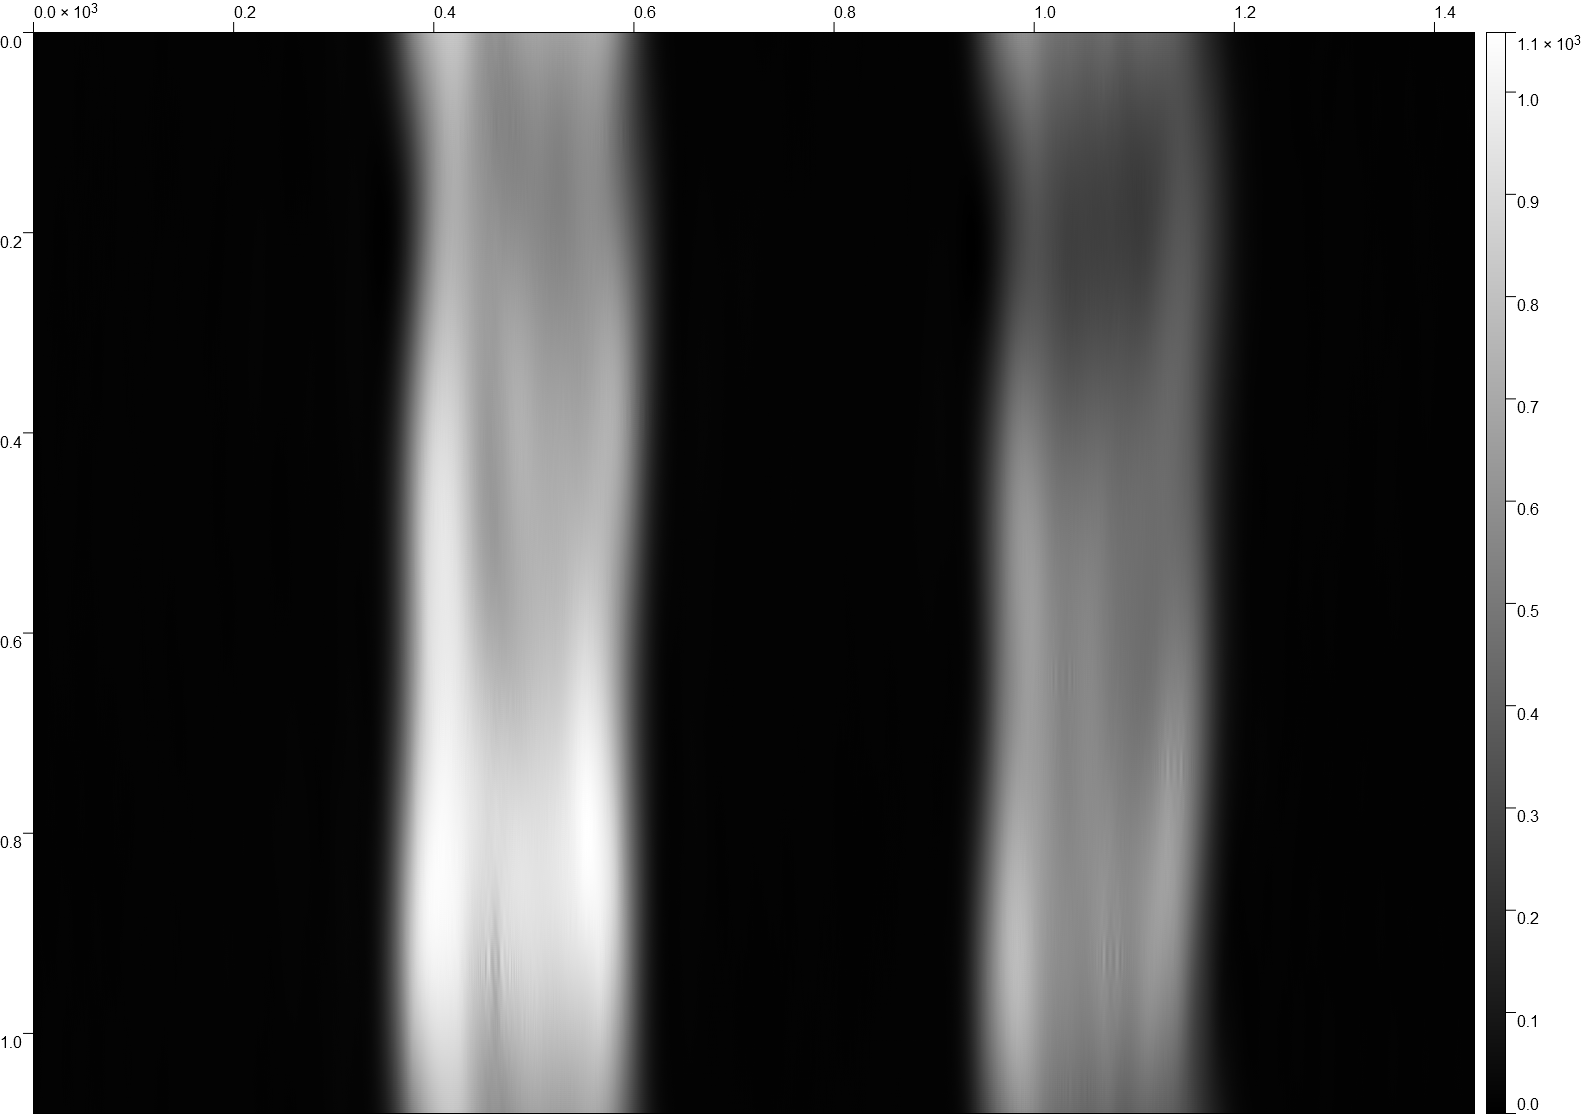
\includegraphics[width=0.48\textwidth]{graphics/aufnahmen/objektbild_doppelspalt_0_1_2_2024-03-14T11-43-09.604_clear.png}}
  \hfill
  \subfloat[0. - 3. Beugungsmaximum]{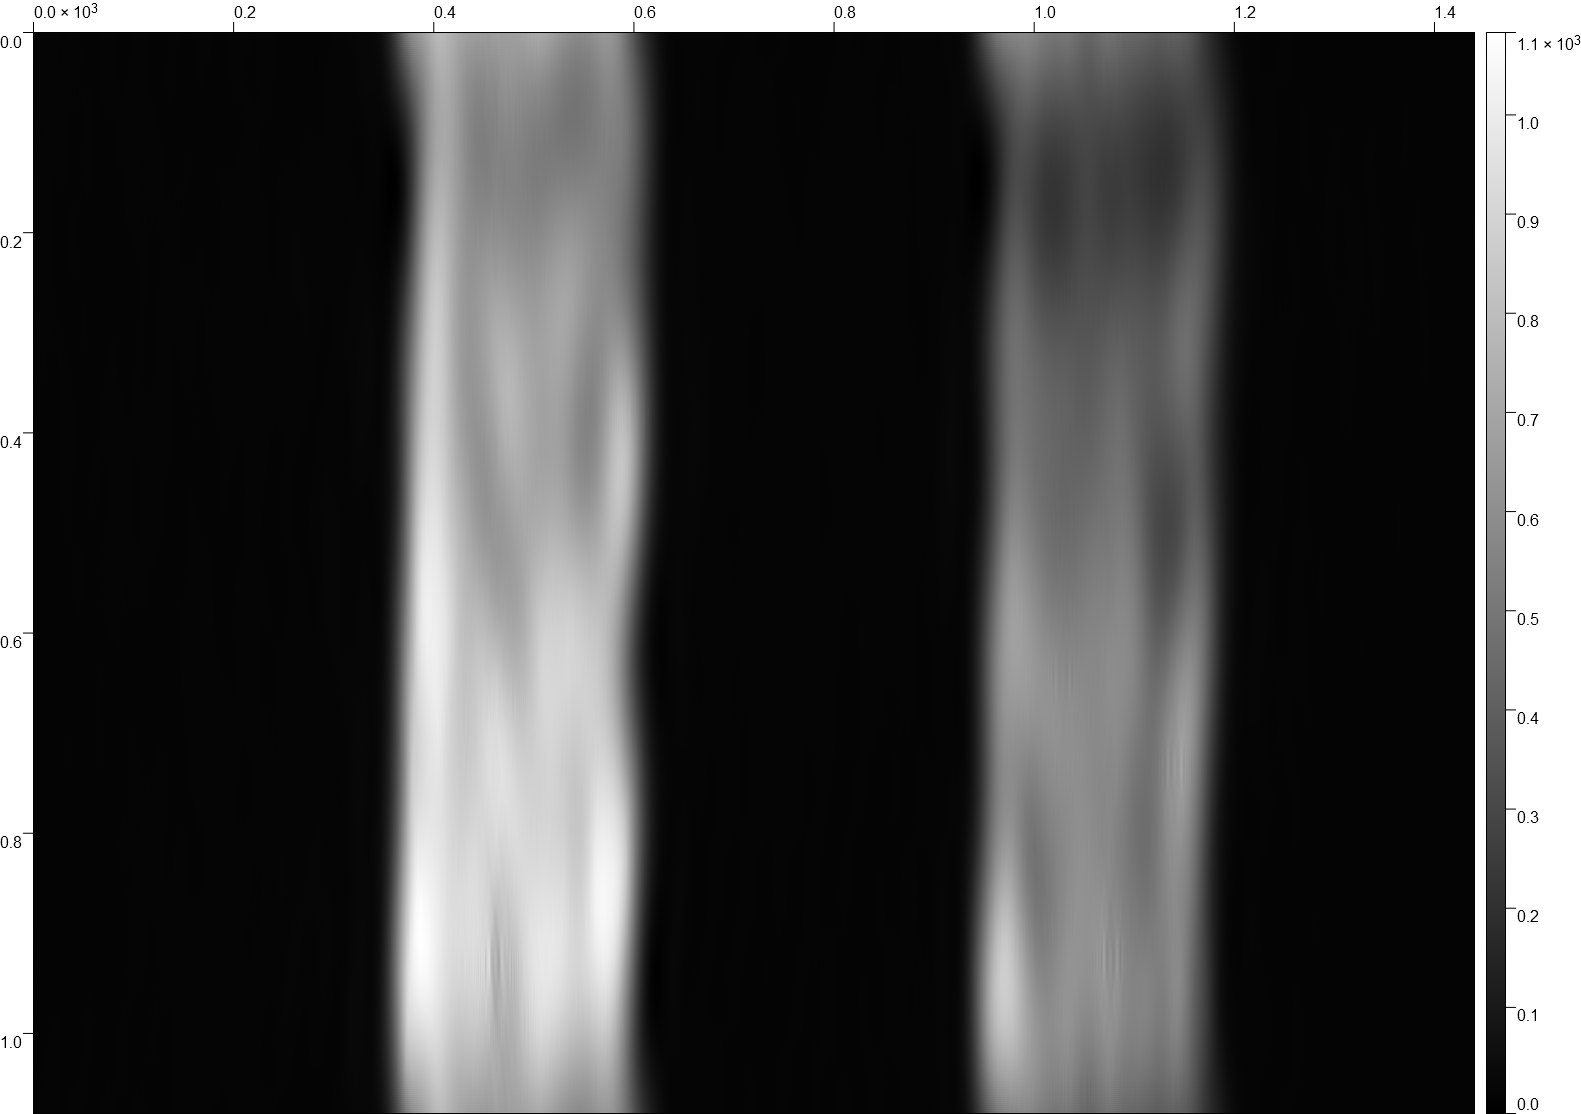
\includegraphics[width=0.48\textwidth]{graphics/aufnahmen/objektbild_doppelspalt_0_1_2_3_2024-03-14T11-43-54.796_clear.png}}
  \hfill
  \subfloat[alle Beugungsmaxima]{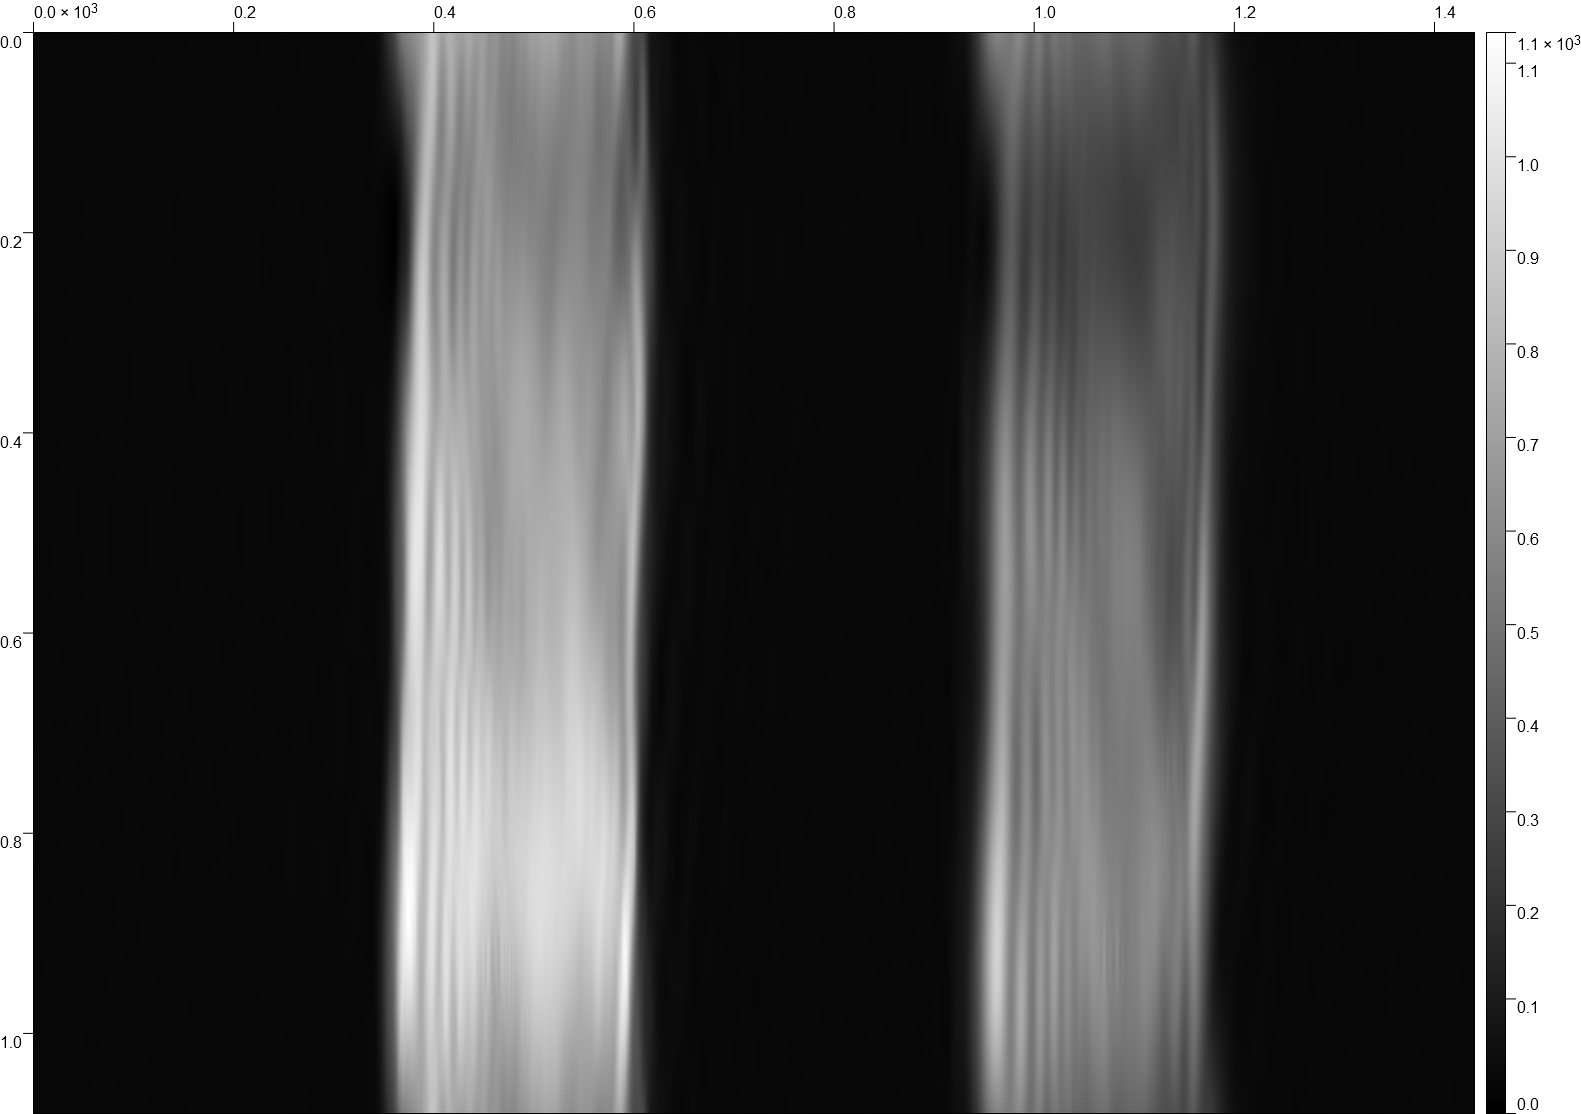
\includegraphics[width=0.48\textwidth]{graphics/aufnahmen/objektbild_doppelspalt_full_2024-03-14T11-44-22.653_clear.png}}
  \hfill
  \subfloat[keine Beugungsmaxima]{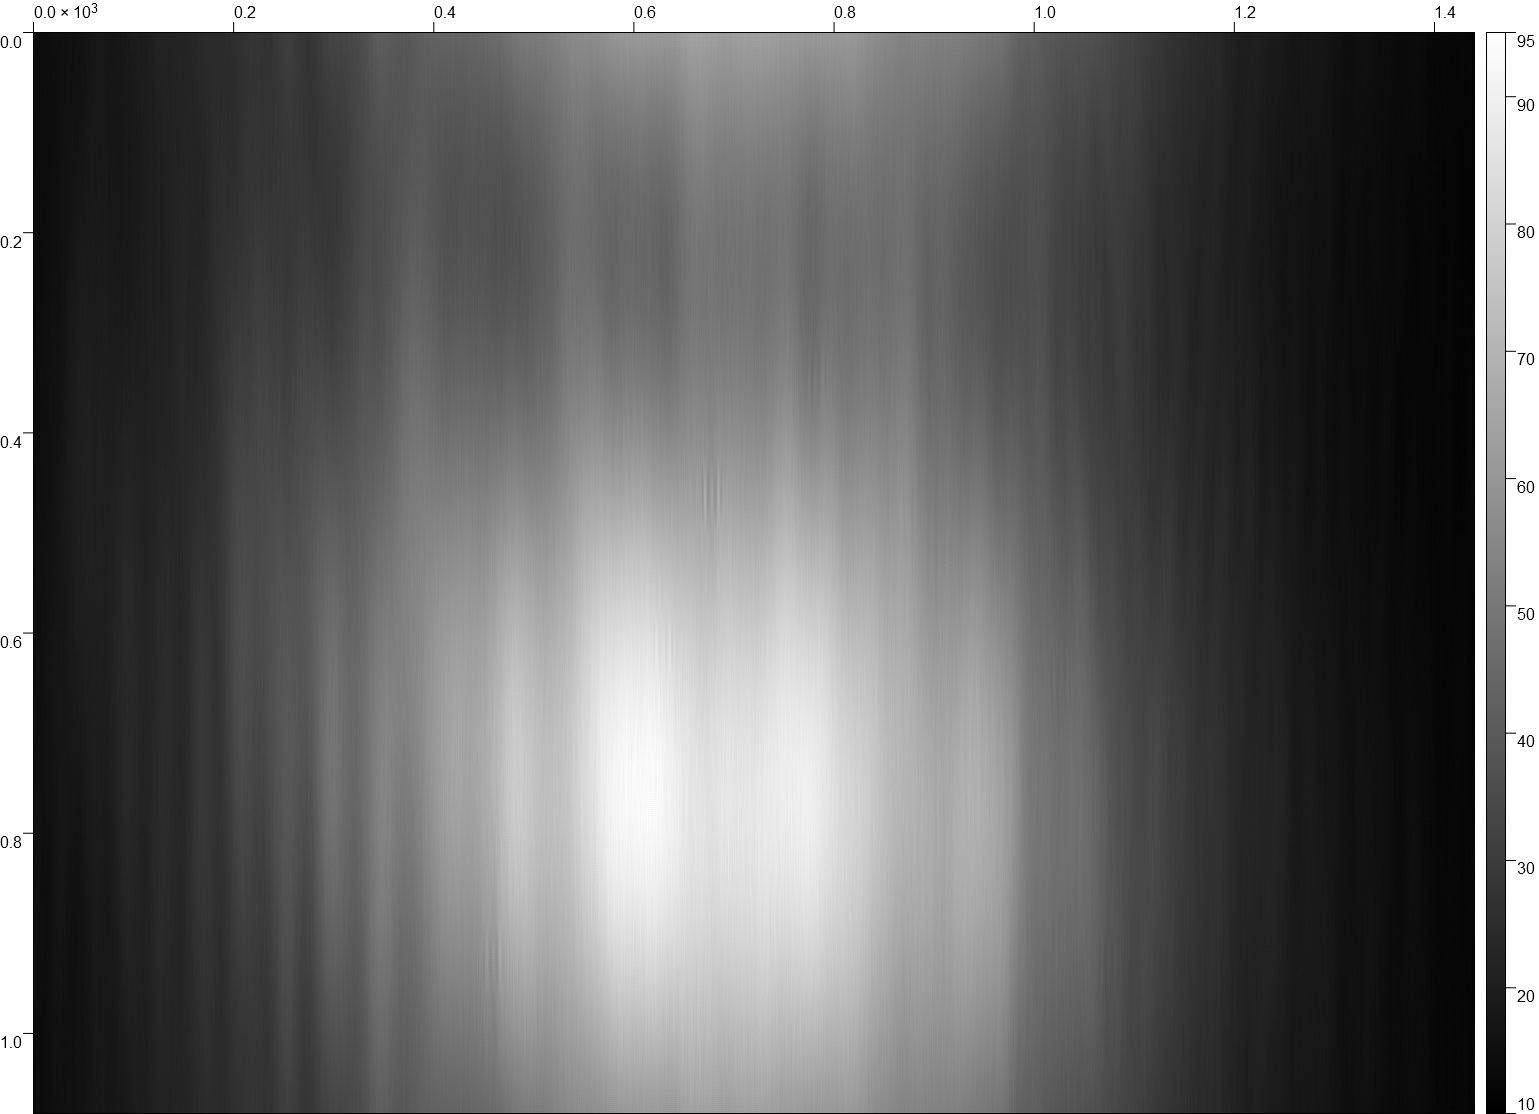
\includegraphics[width=0.48\textwidth]{graphics/aufnahmen/objektbild_doppelspalt_ununterscheidbar_2024-03-14T11-25-09.972_clear.png}}
  \hfill
  \caption{Aufgenommene Objektbilder - Doppelspalt}
  \label{fig:Aufnahmen_Obj_Doppel}
\end{figure}

\clearpage
\newpage
%-------------------------AUSWERTUNG-------------------------
\section{Auswertung}

In dieser Evaluation werden alle Fehler, sofern keine spezifische Angabe gemacht wird, mithilfe der Gauss'schen Fehlerfortpflanzung berechnet. Dies bedeutet, dass ein Wert $F$, der mit der Formel $f(a_1, ..., a_n)$ berechnet wird, den Fehler $\Delta F$ annimmt:

\begin{equation}
    \Delta F = \sqrt{\sum_n \left( \frac{\partial f}{\partial a_n} \cdot \Delta a_n \right)^2}.
\end{equation}

Des Weiteren erfolgen Signifikanztests von zwei Werten $a$ und $a'$ über die folgende Formel:

\begin{equation}
    \sigma = \frac{|a-a'|}{\sqrt{(\Delta a)^2 + (\Delta a')^2}}.
\end{equation}

Die Güte eines Fits wird mit der $\chi^2$-Summe bewertet:

\begin{equation}
    \chi^2 = \sum_i^N \left( \frac{\textit{Funktionswert}_i - \textit{Messwert}_i}{\textit{Fehler}_i} \right)^2
\end{equation}

Auch verwendet wird $\chi^2_{red} = \chi^2 / f$, wobei der Freiheitsgrad $f$ die Anzahl der Messwerte minus die Anzahl der Fitparameter ist. Der auf die Freiheitsgrade normierte Wert soll bei einem guten Fit ungefähr 1 sein.

Die Auswertung sowie Berechnung erfolgen über das dem Dokument angehängte Python-Programm.

\newpage
\subsubsection{Kurze Erwähnung der qualitativen Analyse}

Der erste Teil der Versuchsdurchführung war eine qualitative Analyse einiger Modifizierungen am Objekt sowie dem Analysespalt. Da hier noch keine großen oder in irgendeiner Form komplexen Beobachtungen angestellt wurden, sondern nur der erste Kennenlernmoment mit dem Versuchsaufbau dokumentiert wurde, lässt sich auch nicht viel sagen außer dass alle Beobachtungen der Theorie entsprachen und erwartete Ergebnisse lieferten. Alle der in Tabelle 1 aufgelisteten Beobachtungen waren zu erwarten. 

Einzig hervorzuheben ist eventuell der letzte Punkt, bei dem der Analysespalt durch eine Modeblende ausgetauscht, die den genau umgekehrten Effekt des Spalts hatte: Es wurden nicht höhere Nebenmaxima sondern das nullte Haupmaximum ausgeblendet. Im Objektbild waren dann nur noch die Kanten sichtbar, was daher kommt, dass fast die gesamte ''Füllung'' und Intensität des Objektbilds vom Hauptmaximum kommt und die höheren Nebenmaxima darauf aufbauend die Kanten scharf machen. Bleiben also nur Nebenmaxima übrig, so verschwindet ein Großteil des Bildes und nur die Kanten sind noch zu sehen. 

\newpage

\subsection{Eichung der Abszisse}

Wir beginnen, indem wir zunächst aus unseren Messwerten der Abszisseneichung aus Tabelle 4 des Messprotokolls den Eichungskoeffizient bestimmen. Dazu tragen wir die Analysierspaltbreiten, welche sich mit dem Faktor 2 aus den notierten halben Werten berechnen lassen, gegen die Pixelwerte auf und fitten eine Gerade an die Messwerte, deren Steigung unser Eichkoeffizient $\epsilon$ wird. Der Plot ist zu sehen in Abbildung \ref{fig:Abszisseneichung}, wobei der Fit den folgenden Parameter bestimmt:

\begin{equation}
    \bm{\epsilon = - \alpha = (0,00341 \pm 0,00010) \frac{\textbf{mm}}{\textbf{pixel}}}.
\end{equation}

\begin{figure}[!b]
    \centering
    \resizebox{0.9\textwidth}{!}{
    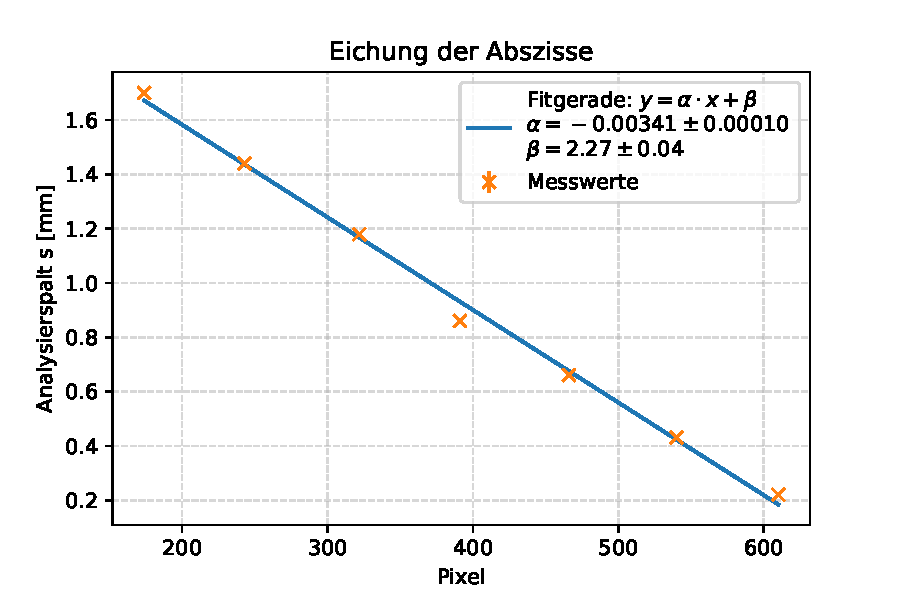
\includegraphics{graphics/plots/Abszisseneichung.pdf}}
    \caption{Plot der Abszisseneichung mit Linearem Fit}
    \label{fig:Abszisseneichung}
\end{figure}

\clearpage
\newpage
\subsection{Analyse der Beugungsbilder des Einzelspalts}

Wir möchten nun die von uns ausgemessenen Werte der Lage und Intensität der Maxima und Minima des Einzelspalts mit der Theorie abgleichen.

\subsubsection{Position der Minima und Spaltbreite}

Zunächst tragen wir die in Tabelle 3 zu findenden Werte der x-Positionen der Minima gegen die jeweilige theoretische Ordnungszahl auf. Dies machen wir jeweils einmal für die positiven und für die negativen Ordnungen, an die wir beide jeweils eine Gerade anfitten. Es ergibt sich das in Abbildung \ref{fig:Pos-Ordn_Min} dargestellte Diagramm. Es ist gut zu erkennen, wie beide Geraden etwa symmetrisch von der ungefähren x-Position des Hauptmaximums verlaufen, die etwa bei 632px liegt. Uns interessieren vor allem die Steigungen der Geraden und davon vor allem die absoluten Werte:

\begin{equation}
    \begin{split}
        a_1 = (72,17 \pm 0,28) \frac{\text{Ordn.}}{\text{px}} \\
        a_2 = (73,14 \pm 0,25) \frac{\text{Ordn.}}{\text{px}}
    \end{split}
\end{equation}

\begin{figure}[!b]
    \centering
    \resizebox{0.9\textwidth}{!}{
    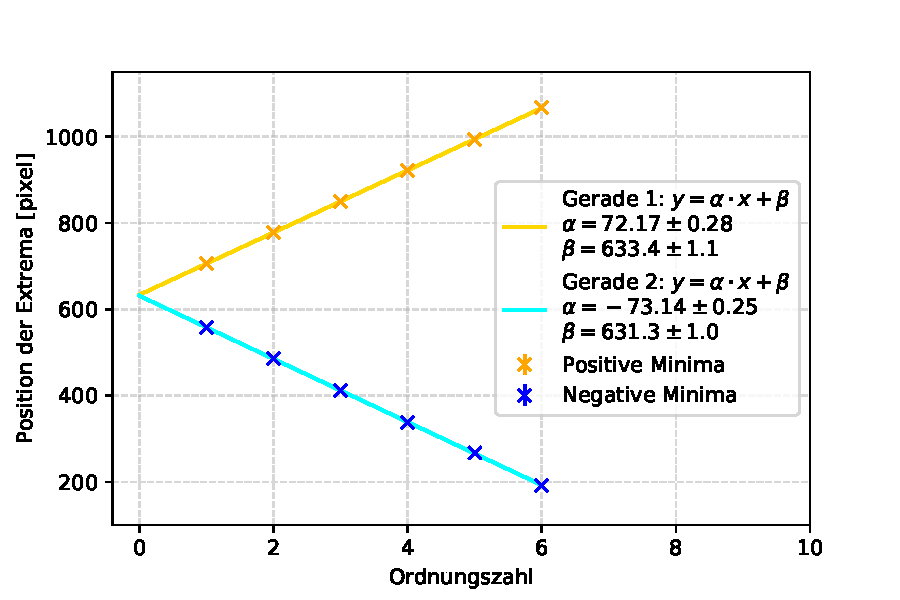
\includegraphics{graphics/plots/Position-Ordnungszahl-Minima.pdf}}
    \caption{Position der Minima gegen die Ordnungszahlen mit Linearen Fits}
    \label{fig:Pos-Ordn_Min}
\end{figure}

\newpage
Aus diesen Geraden kann man nun die Spaltbreite $B$ errechnen. Aus Abbildung \ref{fig:fraunhofer} wird die folgenden Relationen klar:

\begin{equation}
    \begin{split}
        n \lambda &= B \sin{(\alpha)}, \\
        b &= f \tan (\alpha) \approx f \sin{(\alpha)}.
    \end{split}
\end{equation}

Hierbei bezeichnet $\lambda$ die Wellenlänge des Lasers von 532nm und $f=80$mm die Brennweite der Linse L1. Somit ergibt sich mit der Erkenntnis, dass $b/n$ unsere Steigung der Geraden ist, der folgende Zusammenhang:

\begin{equation}
    B = \frac{f n \lambda}{b} = \frac{f \lambda}{a}.
\end{equation}

Unter Berücksichtigung des Eichkoeffizienten der Abszisseneichung $\epsilon$ kann man nun die Spaltbreite errechnen.

\begin{equation}
    \begin{split}
        B &= \frac{f \lambda}{a \epsilon} \\
        \Rightarrow \Delta B &= B \sqrt{\left( \frac{\Delta a}{a} \right)^2 + \left( \frac{\Delta \epsilon}{\epsilon} \right)^2} \\ \\
        &\Rightarrow B_1 = (0,173 \pm 0,005)\text{mm} \\
        &\phantom{\Rightarrow} B_2 = (0,171 \pm 0,005)\text{mm}
    \end{split}
\end{equation}

Wir bilden daraus den Mittelwert und erhalten:

\begin{equation}
    \bm{B = (0,172 \pm 0,005)} \textbf{mm}.
\end{equation}

Der Fehler berechnet sich hierbei aus dem Standardfehler des Mittelwerts sowie den Fehlern der einzelnen Werte: 

\begin{equation}
    \begin{split}
        \Delta \overline{B} &= \sqrt{\sigma_{std}^2 + \left( \frac{1}{N} \sum_{i=1}^N \Delta B_i \right)^2} \\
        \text{mit} \ \ \ \sigma_{std} &= \sqrt{\frac{1}{N(N-1)} \sum_{i=1}^N (\overline{B} - B_i)^2}.
    \end{split}
    \label{eq:FEHLER_MW}
\end{equation}

Da wir diese Form häufig verwenden werden, wird ab sofort immer hierauf verwiesen anstatt unnötigerweise häufig dieselbe Form aufschreiben zu müssen. 

\subsubsection{Position der Maxima}

Mit den Linearen Fits möchten wir nun auch die Position der Maxima überprüfen. Dazu nehmen wir die von uns gemessenen Werte der Positionen der Maxima $x_{max}$ aus Tabelle 3 und berechnen mit der Umkehrfunktion der Linearen Fits die so erhaltenen Ordnungszahlen $n$:

\begin{equation}
    \begin{split}
        n &= \frac{x_{max} - \beta}{\alpha} \\
        \Rightarrow \Delta n &= n \sqrt{\left( \frac{\Delta (x_{max} - \beta)}{(x_{max} - \beta)} \right)^2 + \left( \frac{\Delta \alpha}{\alpha} \right)^2} \\
        &=  n \sqrt{\left( \frac{\sqrt{(\Delta x_{max})^2 + (\Delta \beta)^2}}{(x_{max} - \beta)} \right)^2 + \left( \frac{\Delta \alpha}{\alpha} \right)^2}
    \end{split}
\end{equation}

So erhalten wir die in Tabelle \ref{tab:Einzelsp_Ordn_Maxima} dargestellten Ergebnisse für die Ordnungszahlen der Maxima positiver und negativer Ordnungen. 

\phantom{.}

\begin{table}[!h]
    \centering
    %\resizebox{\textwidth}{!}{
    \begin{tabular}{ccc}
        \hline
        \textbf{Nr.} & $\bm{n_{pos}}$ & $\bm{n_{neg}}$ \\ \hline
             1 &  1,42 $\pm$ 0,07 &  1,43 $\pm$ 0,07 \\
             2 &  2,49 $\pm$ 0,07 &  2,48 $\pm$ 0,07 \\
             3 &  3,47 $\pm$ 0,07 &  3,45 $\pm$ 0,07 \\
             4 &  4,47 $\pm$ 0,07 &  4,48 $\pm$ 0,07 \\
             5 &  5,47 $\pm$ 0,07 &  5,49 $\pm$ 0,07 \\ \hline
    \end{tabular}%}
    \caption{Ordnungszahlen Maxima - positiv und negativ}
    \label{tab:Einzelsp_Ordn_Maxima}
\end{table}

\phantom{.}

Wir berechnen für alle Ordnungen die Mittelwerte aus positiver und negativer Reihe und vergleichen mit den Theoretischen Werten von 1,5, 2,5, ... über einen Signifikanztest, zu sehen in Tabelle \ref{tab:Einzelsp_Ordn_Maxima_mean}.

\phantom{.}

\begin{table}[!h]
    \centering
    %\resizebox{\textwidth}{!}{
    \begin{tabular}{cccc}
        \hline
        \textbf{Nr.} & $\bm{\overline{n}}$ & $\bm{n_{lit}}$ & $\bm{\sigma_n}$ \\ \hline
             1 & 1,42 $\pm$ 0,07 &   1,5 &  1,08 \\
             2 & 2,48 $\pm$ 0,07 &   2,5 &  0,23 \\
             3 & 3,46 $\pm$ 0,07 &   3,5 &  0,54 \\
             4 & 4,47 $\pm$ 0,07 &   4,5 &  0,38 \\
             5 & 5,48 $\pm$ 0,07 &   5,5 &  0,31 \\ \hline
    \end{tabular}%}
    \caption{Ordnungszahlen Maxima Mittelwert und Signifikanztest}
    \label{tab:Einzelsp_Ordn_Maxima_mean}
\end{table}

\phantom{.}

Zusätzlich tragen wir die Maxima mit den berechneten Ordnungszahlen auch in das Diagramm ein und erhalten Abbildung \ref{fig:Pos-Ordn_Min_Max}.

\begin{figure}[!b]
    \centering
    \resizebox{0.9\textwidth}{!}{
    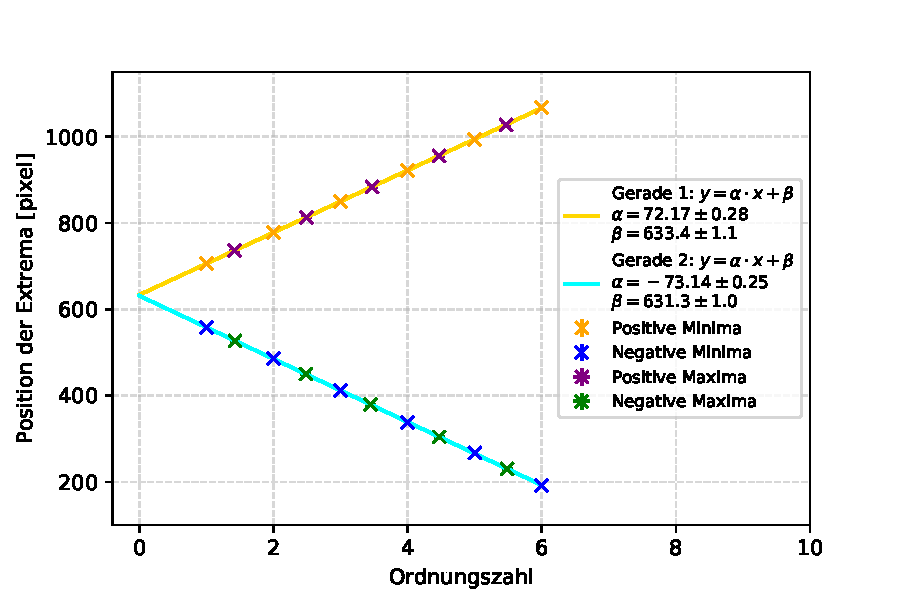
\includegraphics{graphics/plots/Position-Ordnungszahl-Min+Max.pdf}}
    \caption{Position der Minima \& Maxima gegen die Ordnungszahlen}
    \label{fig:Pos-Ordn_Min_Max}
\end{figure}

\clearpage
\subsubsection{Intensitätsverhältnisse}

Zuletzt wollen wir die gemessenen Intensitäten mit den theoretisch zu erwartenden Werten vergleichen. Dazu berechnen wir zunächst die Verhältnisse von den Nebenmaxima zum Hauptmaximum. Dabei gehen wir wie folgt vor:

Zuerst berechnen wir mit den Werten aus Tabelle 2, ergo von der Messung in der das Hauptmaximum und 1. Nebenmaximum vermessen wurde, das Verhältnis von genau den beiden Maxima $I_{01}$ unter Berücksichtigung des eingestellten Blacklevels von $+9$:

\begin{equation}
    \begin{split}
        I_{01} &= \frac{I_1 - 9}{I_0 - 9}, \\
        \Rightarrow \Delta I_{01} &= I_{01} \sqrt{\left( \frac{\Delta I}{I_0 - 9} \right)^2 + \left( \frac{\Delta I}{I_1 - 9} \right)^2}.
    \end{split}
\end{equation}

Dabit können wir nun die Verhältnisse aller Nebenmaxima zum Hauptmaximum bestimmen, indem wir die Messungen aus Tabelle 3 aller Nebenmaxima nehmen, daraus die Verhältnisse der höheren Nebenmaxima zum 1. bestimmen und mit dem soeben bestimmten Verhältnis $I_{01}$  multiplizieren:

\begin{equation}
    \begin{split}
        I_{0n} &= I_{01} \cdot \frac{I_n - 9}{I_1 - 9}, \\
        \Rightarrow \Delta I_{0n} &= I_{0n} \sqrt{\left( \frac{\Delta I_{01}}{I_{01}} \right)^2 + \left( \frac{\Delta I}{I_n - 9} \right)^2 + \left( \frac{\Delta I}{I_0 - 9} \right)^2}.
    \end{split}
\end{equation}

Wir berechnen also alle Verhältnisse für die positiven sowie die negativen Maxima  und bilden am Ende den Mittelwert aus den beiden Werten gleicher Ordnung. Wir erhalten die Ergebnisse in Tabelle \ref{tab:Einzelsp_RelInten_Mess}.

\begin{table}[!hb]
    \centering
    %\resizebox{\textwidth}{!}{
    \begin{tabular}{cccc}
        \hline
        \textbf{Ordnung} $\bm{n}$ & $\bm{I_{0n,pos}}$ & $\bm{I_{0n,neg}}$ & $\bm{\overline{I}_{0n}}$ \\ \hline
             1 &    0,042 $\pm$ 0,006 &    0,044 $\pm$ 0,006 & 0,043 $\pm$ 0,006 \\
             2 &    0,0159 $\pm$ 0,0021 &    0,0158 $\pm$ 0,002  & 0,0158 $\pm$ 0,0021 \\
             3 &    0,0085 $\pm$ 0,0011 &    0,0082 $\pm$ 0,0011 & 0,0083 $\pm$ 0,0011 \\
             4 &    0,0057 $\pm$ 0,0008 &    0,0047 $\pm$ 0,0006 & 0,0052 $\pm$ 0,0009 \\
             5 &    0,0034 $\pm$ 0,0005 &    0,0032 $\pm$ 0,0005 & 0,0033 $\pm$ 0,0005 \\ \hline
    \end{tabular}%}
    \caption{Relative Intensitäten der Nebenmaxima $n$-ter Ordnung zum Hauptmaximum - Messungen}
    \label{tab:Einzelsp_RelInten_Mess}
\end{table}

Anschließend berechnen wir die theoretisch zu erwarteten Werte für die Verhältnisse. Dazu berechnen wir für alle Ordnungen $n = 1, ... , 5$ die Maxima der Intensitätsverteilung $\text{sinc}(x)^2$, wobei gilt:

\begin{equation}
    \begin{split}
        x_n &= (n + 0,5) \pi - \frac{1}{(n + 0,5) \pi}, \\
        \Rightarrow I_{0n,theo} &= \frac{\sin{(x_n)}^2}{{(x_n)}^2}.
    \end{split}
\end{equation}

Diese Werte, zu sehen in Tabelle \ref{tab:Einzelsp_RelInten_Theo&sign}, vergleichen wir nun über Signifikanztests mit den Werten aus der Messung, was auch in die gleiche Tabelle eingetragen wird. 

\begin{table}[!hb]
    \centering
    %\resizebox{\textwidth}{!}{
    \begin{tabular}{cccc}
        \hline
        \textbf{Ordnung} $\bm{n}$ & $\bm{\overline{I}_{0n}}$ & $\bm{I_{0n,theo}}$ & $\bm{\sigma}$ \\ \hline
             1 & 0,0426 $\pm$ 0,0056 & 0,04718830 &    0,82 \\
             2 & 0,0158 $\pm$ 0,0021 & 0,01648000 &    0,31 \\
             3 & 0,0083 $\pm$ 0,0011 & 0,00834029 &    0,01 \\
             4 & 0,0052 $\pm$ 0,0009 & 0,00502872 &    0,15 \\
             5 & 0,0033 $\pm$ 0,0005 & 0,00336073 &    0,04 \\ \hline
    \end{tabular}%}
    \caption{Relative Intensitäten der Nebenmaxima $n$-ter Ordnung zum Hauptmaximum - Theorie \& Signifikanztests}
    \label{tab:Einzelsp_RelInten_Theo&sign}
\end{table}

Es ist zu erkennen, dass alle Signifikanztests insignifikante Abweichungen innerhalb der $1\sigma$-Umgebung aufweisen. 

\clearpage
\newpage
\subsection{Analyse der Beugungsbilder des Doppelspalts}

Wir wollen nun unsere Aufnahme des Beugungsbilds des Doppelspalts mit der theoretischen Erwartung vergleichen. Dazu erstellen wir zunächst das Beugungsbild des Spalts ($s$) und Doppelspalts ($d$) basierend auf den Funktionen

\begin{equation}
    \begin{split}
        I(x)_s &= \frac{\sin^2{x}}{x^2}, \\
        I(x)_d &= \frac{\sin^2{x}}{x^2} \cos^2{(\pi v x)}.
    \end{split}
\end{equation}

Hierbei bezeichnet $a$ die Anzahl der Nebenmaxima die dargestellt werden sollen und $v$ das Verhältnis vom Spaltabstand zur Spaltbreite. Wir setzen $a=1$, um das Bild bis zum ersten Nebenmaximum der Spaltfunktion zu generieren und verwenden für $v$ unsere in Teil 5 im Messprotokoll verwendeten Werte $d_1$ bis $d_3$, wobei wir den Mittelwert $\overline{d}$ aus den beiden Spaltbreiten $d_1$ \& $d_2$ bilden: $v = d_3/\overline{d} = 2,475$. So erhalten wir das in Abbildung \ref{fig:Beug_d_s_theo} dargestellte Diagramm der Theorie. 

\begin{figure}[!b]
    \centering
    \resizebox{0.9\textwidth}{!}{
    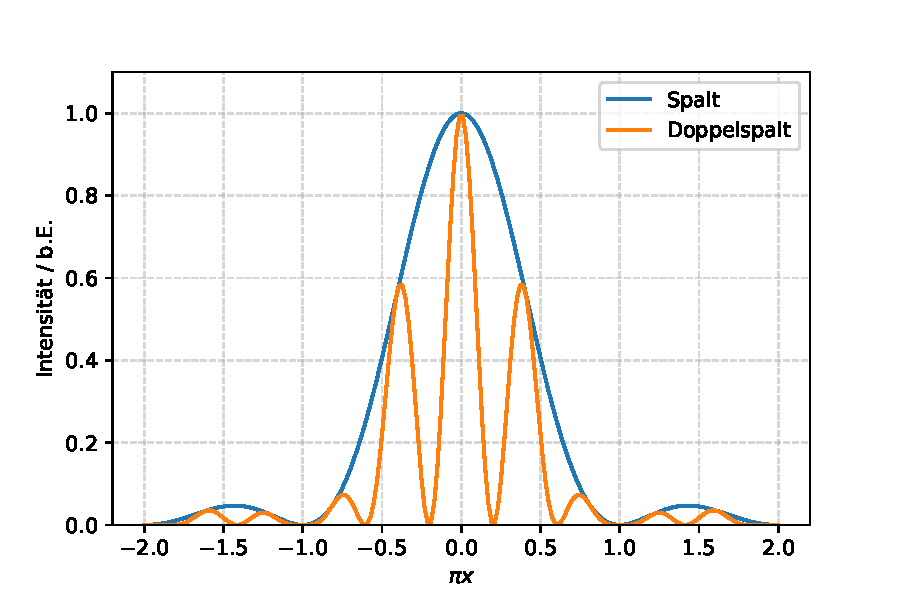
\includegraphics{graphics/plots/Beugung_spalt_doppelspalt_Theo.pdf}}
    \caption{Theoretisches Beugungsbild vom Spalt und Doppelspalt}
    \label{fig:Beug_d_s_theo}
\end{figure}

Zum groben qualitativen Vergleich erstellen wir nun Diagramm \ref{fig:Beug_d_s_vgl}. Oben ist unsere Messung der Doppelspaltbeugung zu sehen und unten die soeben theoretisch bestimmten Formen. Die Messung wurde hierbei auf Position und Intensität des Hauptmaximums unter Berücksichtigung des eingestellten Blacklevels normiert. Es ist gut zu erkennen, dass die Form unserer Messung ziemlich genau der der Theorie entspricht. Die Positionen und relativen Intensitäten der Nebenmaxima stimmen ziemlich genau überein und die Messung ist sogar annähernd perfekt symmetrisch.

\begin{figure}[!t]
    \centering
    \resizebox{0.9\textwidth}{!}{
    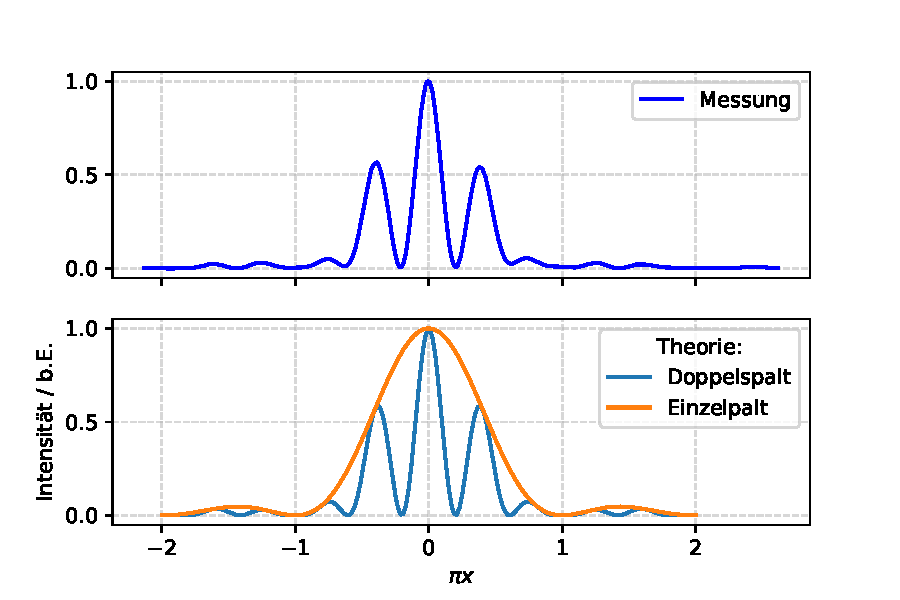
\includegraphics{graphics/plots/Beugung_spalt_doppelspalt_Vergleich.pdf}}
    \caption{Qualitativer Vergleich Theorie und Messung}
    \label{fig:Beug_d_s_vgl}
\end{figure}

Nun wollen wir aber nicht nur qualitativ, sondern auch quantitativ die Messung mit der Theorie vergleichen. Dazu dienen die in Tabelle 5 ausgemessenen Intensitäten der Nebenmaxima, aus denen wir analog zum Einzelspalt die relativen Intensitäten bestimmen. Wir gehen dazu bis zum positiven und negativen Maximum 2. Ordnung und berechnen also:

\begin{equation}
    \begin{split}
        I_{0i} &= \frac{I_i}{I_0}, \\
        \Rightarrow \Delta I_{0i} &= I_{0i} \sqrt{\left( \frac{\Delta I}{I_i} \right)^2 + \left( \frac{\Delta I}{I_0} \right)^2}.
    \end{split}
\end{equation}

So berechnen wir die Werte für die Nebenmaxima 1 und 2 positiver und negativer Ordnung:

\begin{equation}
    \begin{split}
        I_{01,p} &= 0,542 \pm 0,007 \\
        I_{01,n} &= 0,565 \pm 0,008 \\
        I_{02,p} &= 0,056 \pm 0,007 \\
        I_{02,n} &= 0,050 \pm 0,007
    \end{split}
\end{equation}

Wir bilden die Mittelwerte aus den positiven und negativen Werten gleicher Ordnung, der Fehler berechnet sich analog zu Gleichung \ref{eq:FEHLER_MW}, und erhalten:

\begin{equation}
    \begin{split}
        I_{01} &= 0,554 \pm 0,014 \\
        I_{02} &= 0,053 \pm 0,007
    \end{split}
\end{equation}

Die theoretischen Werte errechnen wir aus dem berechneten Beugungsbild. Wir lassen uns mithilfe des Scipy-Packages die Peaks des Bilds bestimmen und ausgeben, dabei erhalten wir die folgenden relativen Intensitäten:

\begin{equation}
    \begin{split}
        I_{01,theo} &= 0,5858 \\
        I_{02,theo} &= 0,0734
    \end{split}
\end{equation}

\begin{figure}[!b]
    \centering
    \resizebox{0.9\textwidth}{!}{
    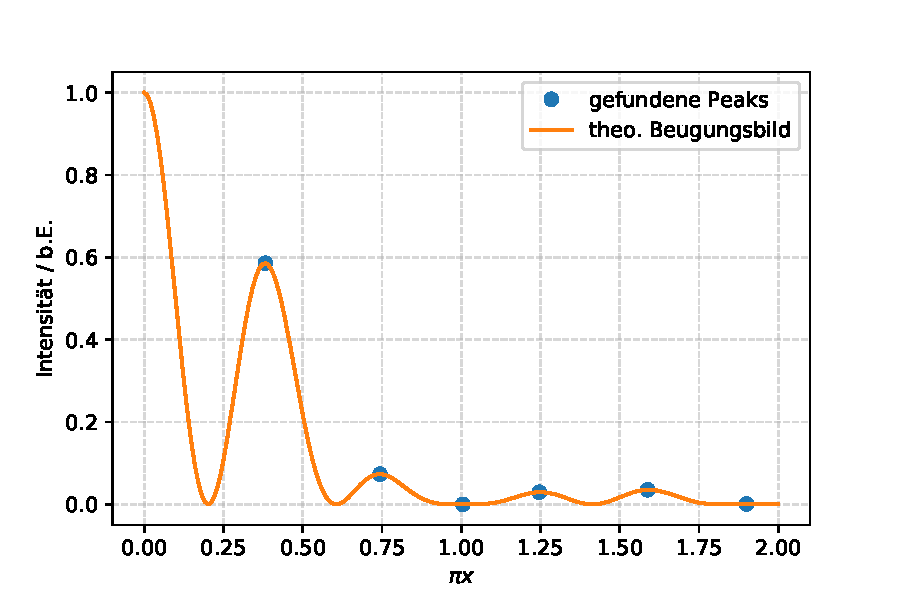
\includegraphics{graphics/plots/Beugung_doppelspalt_Theo_Peaks.pdf}}
    \caption{Theoretisches Beugungsbild mit Peaks}
    \label{fig:Beug_d_peaks}
\end{figure}

In Abbildung \ref{fig:Beug_d_peaks} ist das zugehörige Diagramm des theoretischen Beugungsbilds mit den eingetragenen Peaks zu sehen. 

Wir vergleichen die Werte der Messung und Theorie über Signifikanztests und erhalten:

\begin{equation}
    \begin{split}
        \sigma_{I_{01,theo}} &= 2,30 \\
        \sigma_{I_{02,theo}} &= 2,78
    \end{split}
\end{equation}

Beide sind zwar etwas erhöht, aber immer noch insignifikante Abweichungen innerhalb der $3\sigma$-Umgebung. 


\clearpage
\newpage
\subsection{Analyse der Objektbilder des Einzelspalts}

Um unsere Messungen der Objektbilder des Einzelspalts zu vergleichen berechnen wir erneut die theoretisch erwarteten Objektbilder. Dies geschieht über die in den Grundlagen hergeleitete Form:

\begin{equation}
    \begin{split}
        f_{mod,s} (y) &= \frac{d}{\pi} \int_0^{k_{y,n}} \frac{\sin{(k_y d / 2)}}{k_y d / 2} \ \cos{(k_y y)} \ dk_y, \\
        k_{y,n} &= k_0 \sin{(\alpha_n)} = k_0 n \frac{\lambda}{d} = 2 n \frac{\pi}{d}.
    \end{split}
\end{equation}

Wir setzen für unsere Bilder die Spaltbreite $d=249$pixel und erstellen die Bilder für $n=0,...,3$ sowie einmal $n=30$ als Simulation des weit geöffneten Spalts. 

Zusätzlich bestimmen wir aus unseren Messungen bis zur dritten zugelassenen Nebenordnung noch die normierten Diagramme, indem wir die x-Position jeweils um das Zentrum des Musters auf die 0 verschieben und die Intensität auf das Maximum der Messung bei der nullten Ordnung normieren $I_{norm} = 592$.

Somit haben wir nun einige Diagramme, die folgendermaßen auf den nächsten Seiten zu sehen sind: \\ In Abbildung \ref{fig:Obj_s_Mess} sind zunächst unsere direkten unnormierten Messungen bis zum dritten Nebenmaximum dargestellt. Anschließend sind in Abbildung \ref{fig:Obj_s_full} das gemessene Spaltbild bei weit geöffnetem Analysespalt sowie das theoretische Bild bei $n=30$ zu sehen. Zuletzt stellt Abbildung \ref{fig:Obj_s_Theo&Norm} die theoretischen Bilder (links) den normierten Messungen (rechts) zum ersten qualitativen Vergleich gegenüber.  

\newpage

\begin{figure}[p]
  \centering
  \subfloat[$n = 0$]{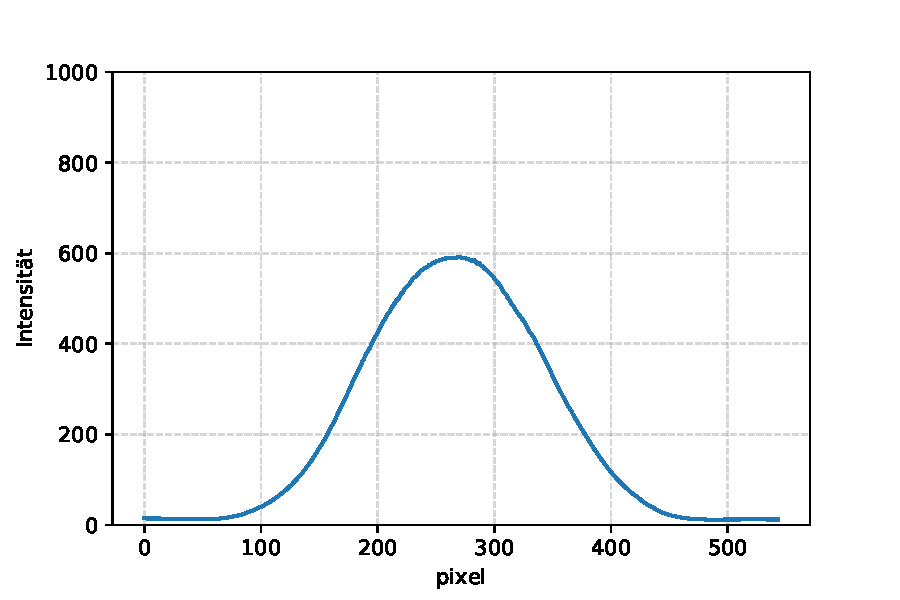
\includegraphics[width=0.48\textwidth]{graphics/plots - obj s/Messung_Obj_Einzelspalt_000.pdf}}
  \hfill
  \subfloat[$n = 1$]{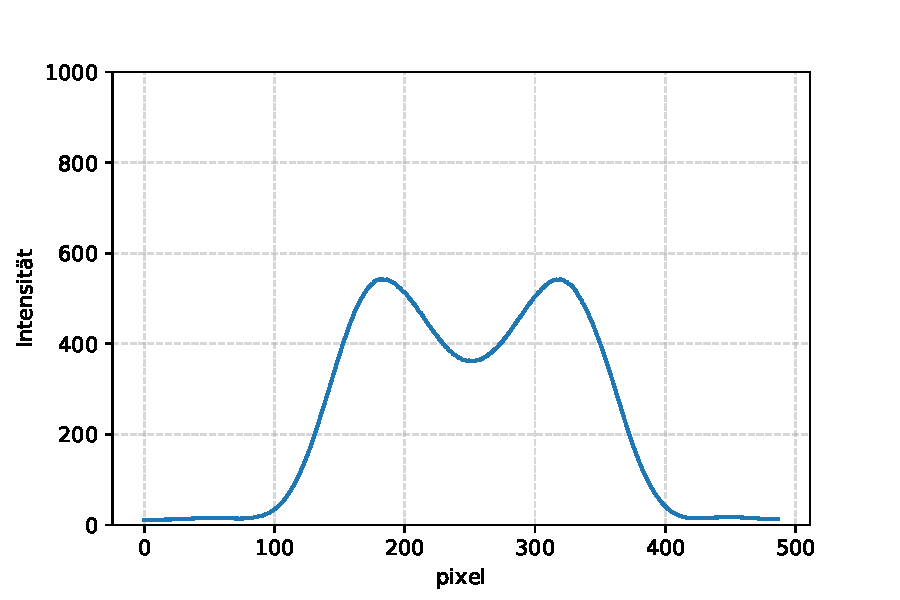
\includegraphics[width=0.48\textwidth]{graphics/plots - obj s/Messung_Obj_Einzelspalt_001.pdf}}
  \hfill
  \subfloat[$n = 2$]{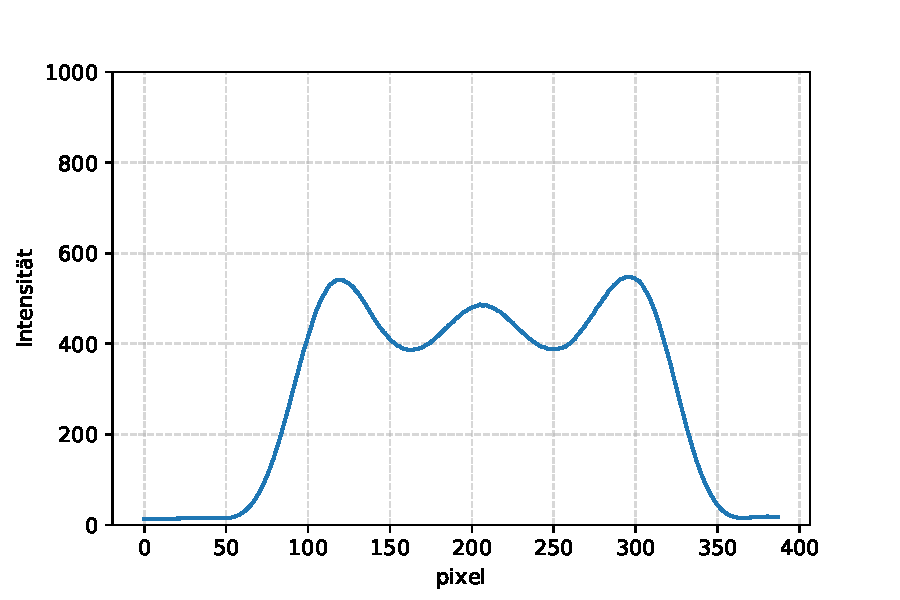
\includegraphics[width=0.48\textwidth]{graphics/plots - obj s/Messung_Obj_Einzelspalt_002.pdf}}
  \hfill
  \subfloat[$n = 3$]{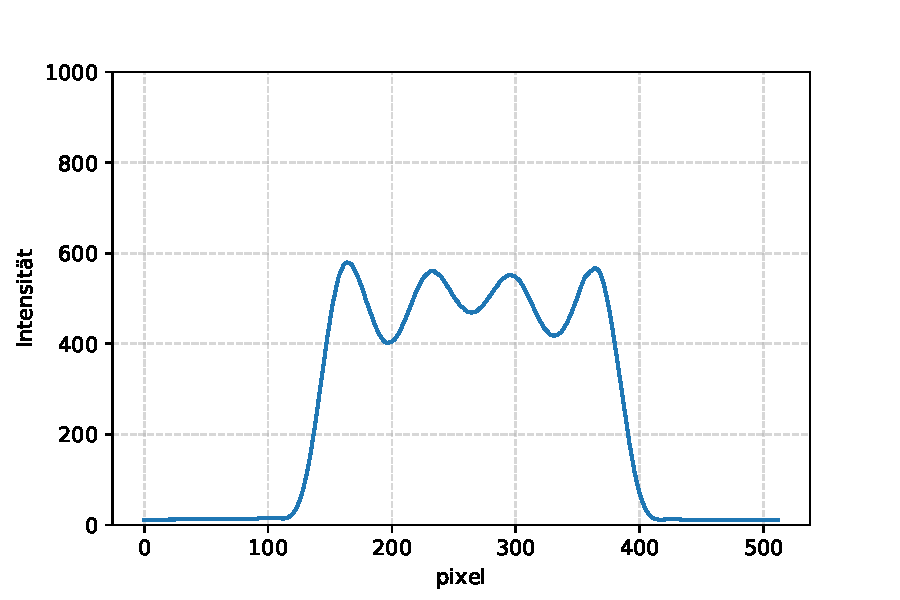
\includegraphics[width=0.48\textwidth]{graphics/plots - obj s/Messung_Obj_Einzelspalt_003.pdf}}
  \hfill
  \caption{Einzelspalt - Messungen bei zugelassenen Maximum $n$-ter Ordnung}
  \label{fig:Obj_s_Mess}
\end{figure}

\begin{figure}[p]
  \centering
  \subfloat[Theorie]{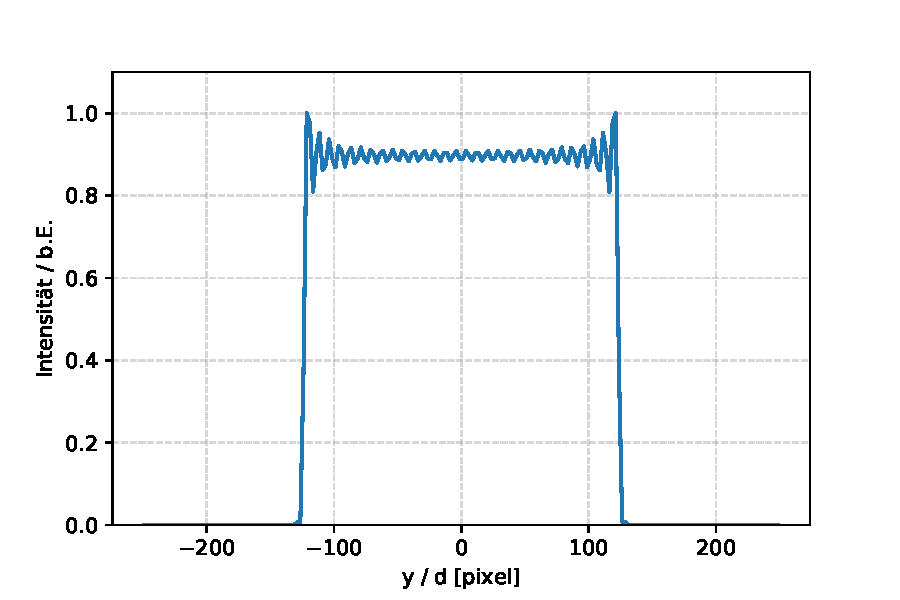
\includegraphics[width=0.48\textwidth]{graphics/plots - obj s/Theo_Obj_Einzelspalt_999.pdf}}
  \hfill
  \subfloat[Messung]{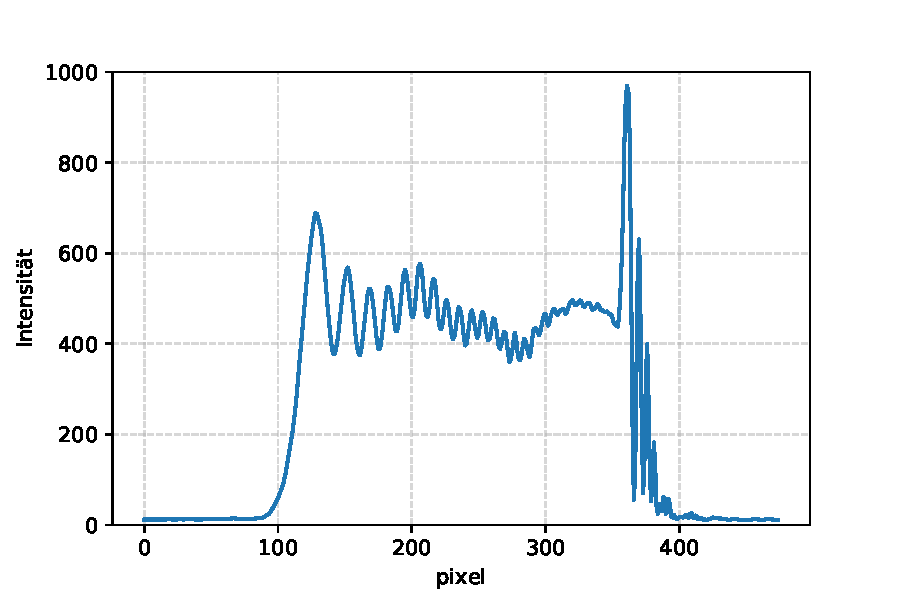
\includegraphics[width=0.48\textwidth]{graphics/plots - obj s/Messung_Obj_Einzelspalt_999.pdf}}
  \hfill
  \caption{Einzelspalt - Theorie \& Messung bei vielen Ordnungen}
  \label{fig:Obj_s_full}
\end{figure}

\clearpage
\newpage

\begin{figure}[p]
  \centering
  \subfloat[Theorie $n = 0$]{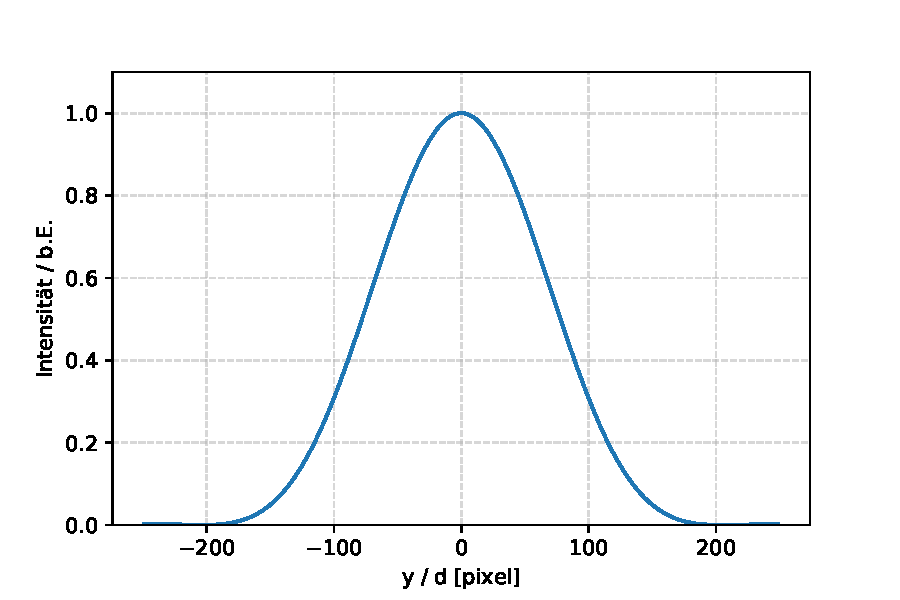
\includegraphics[width=0.48\textwidth]{graphics/plots - obj s/Theo_Obj_Einzelspalt_001.pdf}}
  \hfill
  \subfloat[Normierung $n = 0$]{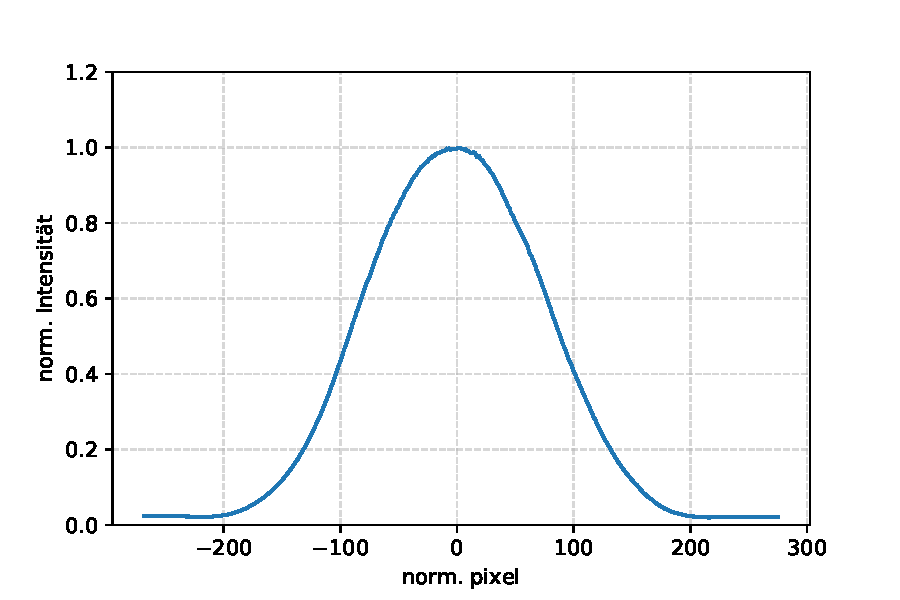
\includegraphics[width=0.48\textwidth]{graphics/plots - obj s/Normierung_Obj_Einzelspalt_000.pdf}}
  \hfill
  \subfloat[Theorie $n = 1$]{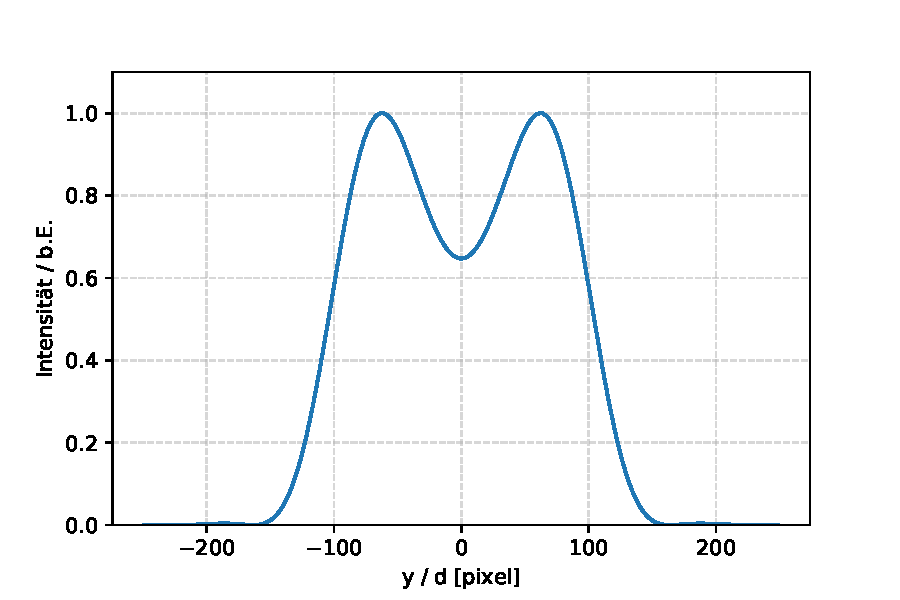
\includegraphics[width=0.48\textwidth]{graphics/plots - obj s/Theo_Obj_Einzelspalt_002.pdf}}
  \hfill
  \subfloat[Normierung $n = 1$]{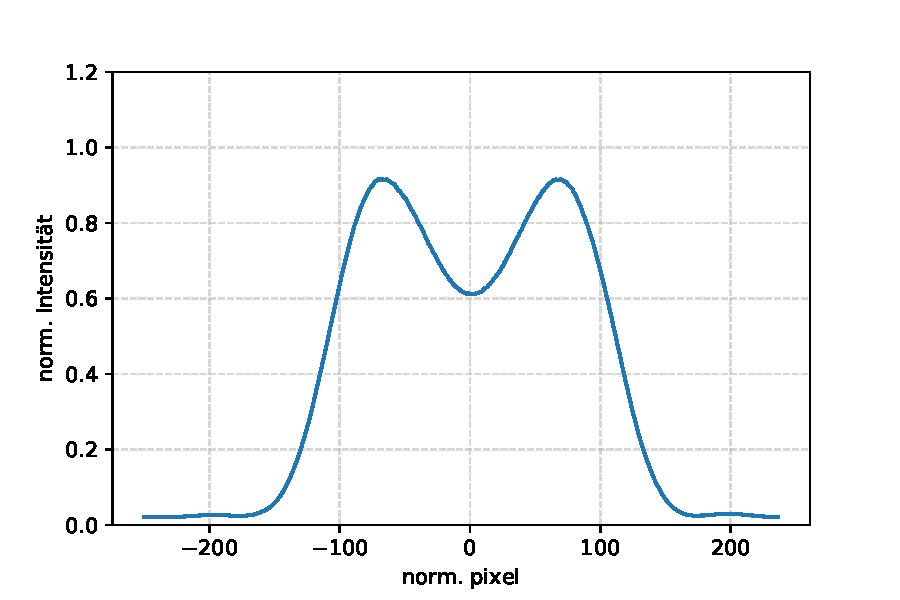
\includegraphics[width=0.48\textwidth]{graphics/plots - obj s/Normierung_Obj_Einzelspalt_001.pdf}}
  \hfill
  \subfloat[Theorie $n = 2$]{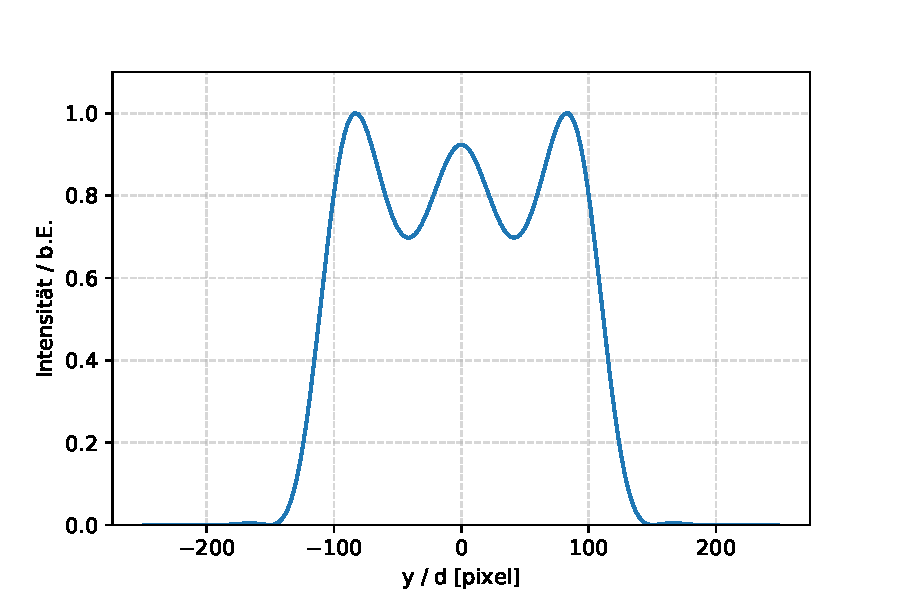
\includegraphics[width=0.48\textwidth]{graphics/plots - obj s/Theo_Obj_Einzelspalt_003.pdf}}
  \hfill
  \subfloat[Normierung $n = 2$]{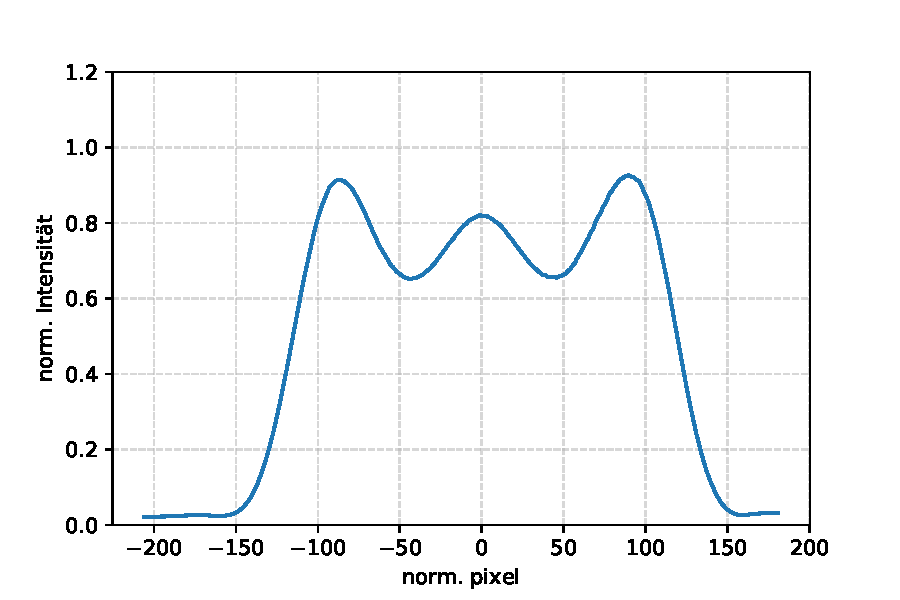
\includegraphics[width=0.48\textwidth]{graphics/plots - obj s/Normierung_Obj_Einzelspalt_002.pdf}}
  \hfill
  \subfloat[Theorie $n = 3$]{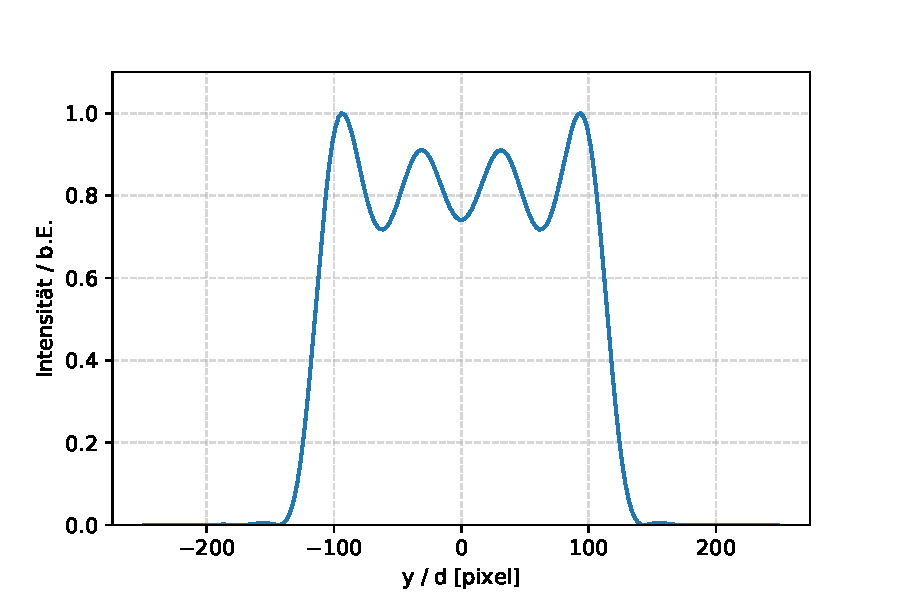
\includegraphics[width=0.48\textwidth]{graphics/plots - obj s/Theo_Obj_Einzelspalt_004.pdf}}
  \hfill
  \subfloat[Normierung $n = 3$]{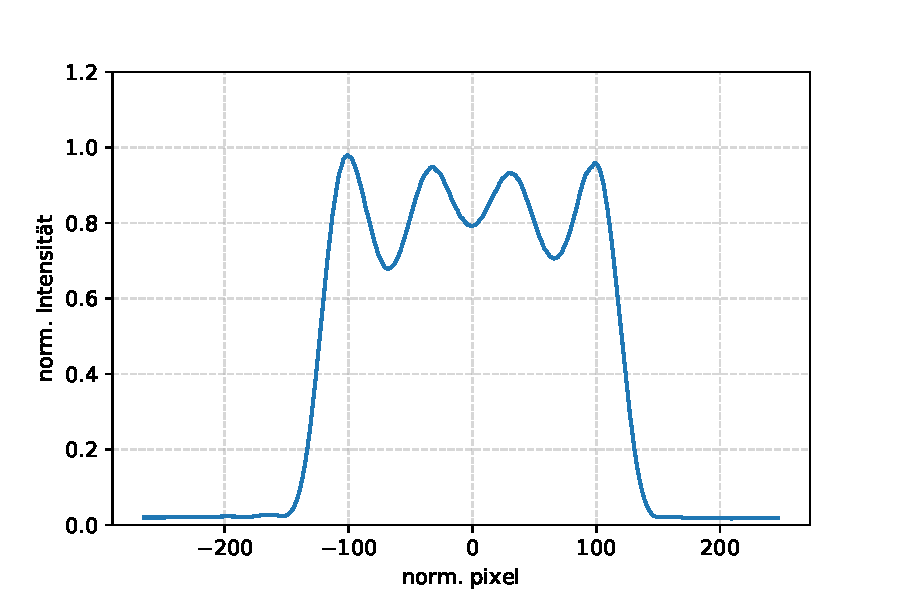
\includegraphics[width=0.48\textwidth]{graphics/plots - obj s/Normierung_Obj_Einzelspalt_003.pdf}}
  \hfill
  \caption{Einzelspalt - Theorie \& Normierung bei zugelassenen Maximum $n$-ter Ordnung}
  \label{fig:Obj_s_Theo&Norm}
\end{figure}

\clearpage
\newpage

Es ist im direkten qualitativen Vergleich gut zu erkennen, dass alle gemessenen Beugungsbilder recht gut mit der Theorie übereinstimmen. Die grundlegende Form stimmt eigentlich immer überein und die Lage sowie Position der Maxima und Minima erscheint sinnvoll. Lediglich beim weit geöffneten Spaltbild stellte konnte eine deutliche Abweichung auf der rechten Seite beobachtete werden. Hierbei wurde schon während des Versuchs festgestellt, dass sich eine Art helle Linie an der rechten kante des Spalts bildet beim weiten Öffnen des Analysespalts. Daher kommen die in Abbildung \ref{fig:Obj_s_full}b auf der rechten Seite sichtbaren sehr hohen Peaks und Verzerrungen. Woher genau diese Anomalie kam ist wie gesagt sehr unklar, jedoch werden keine weiteren quantitativen Vergleiche bei dieser Einstellung gemacht, weshalb es hier auch nicht weiter von großem Belangen sein soll.

Wo allerdings noch quantitativ die Messungen verglichen werden sollen ist bei den Bildern bis zum dritten zugelassen Nebenmaximum. Dazu lesen wir erneut mit dem Scipy-Package die Peaks der normierten Messungsbilder aus. Wir sind wieder an den Intensitäten interessiert und betrachten die der Maxima und Minima in den Objektbildern. Als Fehler schätzen wir hier großzügig $\Delta I = 0,03$, was etwa unserer manuellen Ablesegenauigkeit aus den Diagrammen entsprechen würde. Auf analoge Weise bestimmen wir rechnerich die Intensitäten der Maxima und Minima der theoretischen Objektbilder, woraufhin wir die zueinander gehörenden Maxima und Minima der Messung und Theorie wie gewohnt über Signifikanztests vergleichen. In Tabelle \ref{tab:Einzelsp_Obj_Maxima} sind alle Maxima und in \ref{tab:Einzelsp_Obj_Minima} alle Minima aufgelistet.  

Es ist zu erkennen, dass nur ein Maximum, nämlich das Mittlere des Bilds bis zur 2ten Ordnung, von allen Werten eine signifikante Abweichung von Theoriewert aufweist. Alle anderen Maxima und Minima liegen innerhalb der $3\sigma$-Umgebung und sind somit insignifikant. Es fällt jedoch auf, dass alle Intensitätsprofile höherer Ordnungen bei Normierung auf das Maximum bei nullter Ordnung etwas schwächer sind als erwartet. Während in der Theorie die Peaks am Rand immer bei 1 stehen bleiben sollten, fallen diese und somit das gesamte Bild bei uns etwas nach unten ab, was im Endeffekt auch bei dem einen Maximum für eine signifikante Abweichung führt. Jedoch ist es schwierig hier auf einen systematischen Fehler zu schließen, da bei der Messung mit 3 zugelassenen Nebenmaxima die Intensität der Randpeaks praktisch wieder nahezu auf 1 angestiegen ist, wodurch es sich also eher nicht um eine systematische Verringerung der Intensität handelt. Eine Idee wäre eventuell, dass der Graufilter im Strahlengang hinter der Lichtquelle eventuell Unregelmäßigkeiten aufweist, die sich beim mehrfachen Einsetzen und Rausheben bei diesem Versuchsteil bemerkbar gemacht haben können. Abgesehen davon passen die gemessenen Profile aber von Form und Lage wie erwähnt ziemlich gut zu den theoretisch erwarteten Bildern.  

Zuletzt lässt sich noch erwähnen, dass die Intensität im Zentrum des Objektbilds mit steigenden zugelassenen Ordnungen abnimmt. Dies kommt davon, dass die höheren Ordnungen in der Bildmitte destruktiv interferieren.


\begin{table}[!p]
    \centering
    %\resizebox{\textwidth}{!}{
    \begin{tabular}{cccc}
        \hline
        \textbf{Ordnung} & $\bm{I_{meas}}$ & $\bm{I_{theo}}$ & $\bm{\sigma}$ \\ \hline
               0 &     1,00 $\pm$ 0,03 &   1,0000 &    0,03 \\ \hline
               1 &     0,92 $\pm$ 0,03 &   1,0000 &    2,8  \\
               1 &     0,92 $\pm$ 0,03 &   1,0000 &    2,81 \\ \hline
               2 &     0,91 $\pm$ 0,03 &   1,0000 &    2,85 \\
               2 &     0,82 $\pm$ 0,03 &   0,9232 &    3,36 \\
               2 &     0,93 $\pm$ 0,03 &   1,0000 &    2,46 \\ \hline
               3 &     0,98 $\pm$ 0,03 &   1,0000 &    0,69 \\
               3 &     0,95 $\pm$ 0,03 &   0,9104 &    1,25 \\
               3 &     0,93 $\pm$ 0,03 &   0,9104 &    0,77 \\
               3 &     0,96 $\pm$ 0,03 &   1,0000 &    1,39 \\ \hline
    \end{tabular}%}
    \caption{Objektbild Einzelspalt - Maxima}
    \label{tab:Einzelsp_Obj_Maxima}
\end{table}

\begin{table}[!p]
    \centering
    %\resizebox{\textwidth}{!}{
    \begin{tabular}{cccc}
        \hline
        \textbf{Ordnung} & $\bm{I_{meas}}$ & $\bm{I_{theo}}$ & $\bm{\sigma}$ \\ \hline
               1 &     0,61 $\pm$ 0,03 &   0,6473 &    1,21 \\ \hline
               2 &     0,65 $\pm$ 0,03 &   0,6973 &    1,53 \\
               2 &     0,66 $\pm$ 0,03 &   0,6973 &    1,41 \\ \hline
               3 &     0,68 $\pm$ 0,03 &   0,7174 &    1,28 \\
               3 &     0,79 $\pm$ 0,03 &   0,7413 &    1,68 \\
               3 &     0,71 $\pm$ 0,03 &   0,7174 &    0,38 \\ \hline
    \end{tabular}%}
    \caption{Objektbild Einzelspalt - Minima}
    \label{tab:Einzelsp_Obj_Minima}
\end{table}

\clearpage
\newpage
\subsection{Analyse der Objektbilder des Doppelspalts}

\subsubsection{Betrachtung der Bilder von nullter bis dritter Ordnung}

Erneut berechnen wir zur Analyse die Normierten Messungen sowie die theoretisch zu erwartenden Bilder. Letzteres verläuft über die folgende Formel:

\begin{equation}
    f_{mod,d} (y) = \frac{2d}{\pi} \int_0^{k_{y,n}} \frac{\sin{(k_y d / 2)}}{k_y d / 2} \ \cos{(k_y y)} \ \cos{(k_y g / 2)} \ dk_y.
\end{equation}

Dabei hat $k_y$ dieselbe Form wie beim Einzelspalt. Die neu eingeführte Variable $g$ bezeichnet den Spaltabstand in Einheiten der Spaltbreite, was sich aus $g= v \cdot d$ ergibt, wobei wir die Spaltbreite $d$ wieder analog zur Analyse des Beugungsbildes des Doppelspalts aus dem Mittelwert der beiden gemessenen Breiten $d_1$ und $d_2$ bestimmen. 

Die normierten Bilder ergeben sich aus den Messungen erneut durch eine Verschiebung in x-Richtung sowie die Normierung auf das jeweilige Intensitätsmaximum der Messungen.

Analog bestimmen wir auch aus den theoretischen und normierten Bildern die Maxima und Minima. Zur Veranschaulichung werden in den Messungen die gefundenen Maxima und Minima eingetragen.   

\newpage

\begin{figure}[p]
  \centering
  \subfloat[$n = 0$]{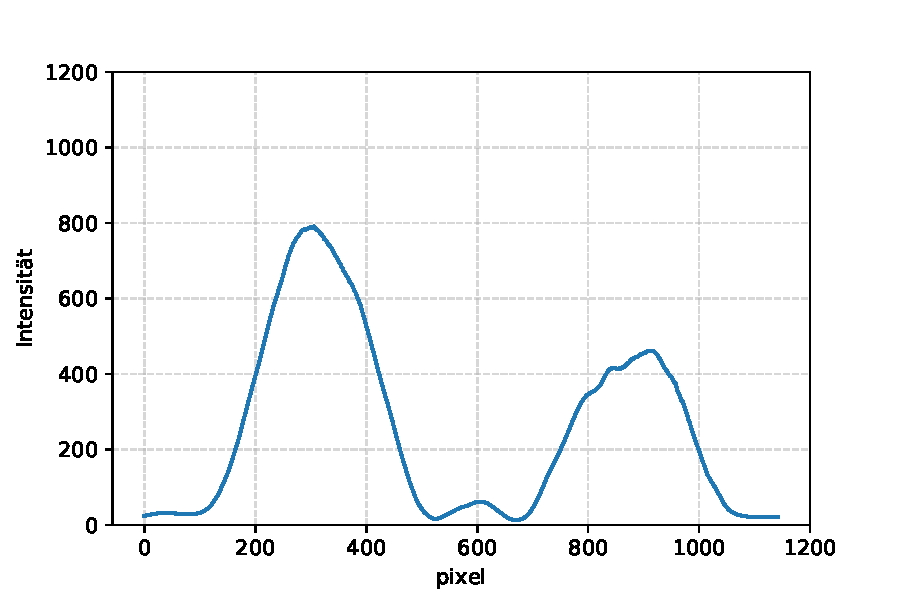
\includegraphics[width=0.48\textwidth]{graphics/plots - obj d/Messung_Obj_Doppelspalt_000.pdf}}
  \hfill
  \subfloat[$n = 1$]{\includegraphics[width=0.48\textwidth]{graphics/plots - obj d/Messung_Obj_Doppelspalt_001.pdf}}
  \hfill
  \subfloat[$n = 2$]{\includegraphics[width=0.48\textwidth]{graphics/plots - obj d/Messung_Obj_Doppelspalt_002.pdf}}
  \hfill
  \subfloat[$n = 3$]{\includegraphics[width=0.48\textwidth]{graphics/plots - obj d/Messung_Obj_Doppelspalt_003.pdf}}
  \hfill
  \subfloat[0te Ordn. abgeschnitten]{\includegraphics[width=0.48\textwidth]{graphics/plots - obj d/Messung_Obj_Doppelspalt_998.pdf}}
  \hfill
  \subfloat[viele Ordnungen]{\includegraphics[width=0.48\textwidth]{graphics/plots - obj d/Messung_Obj_Doppelspalt_999.pdf}}
  \hfill
  \caption{Doppelspalt - Messungen bei zugelassenen Maximum $n$-ter Ordnung}
  \label{fig:Obj_d_Mess}
\end{figure}


\clearpage
\newpage

\begin{figure}[p]
  \centering
  \subfloat[Theorie $n = 0$]{\includegraphics[width=0.48\textwidth]{graphics/plots - obj d/Theo_Obj_Doppelspalt_001.pdf}}
  \hfill
  \subfloat[Normierung $n = 0$]{\includegraphics[width=0.48\textwidth]{graphics/plots - obj d/Normierung_Obj_Doppelspalt_000.pdf}}
  \hfill
  \subfloat[Theorie $n = 1$]{\includegraphics[width=0.48\textwidth]{graphics/plots - obj d/Theo_Obj_Doppelspalt_002.pdf}}
  \hfill
  \subfloat[Normierung $n = 1$]{\includegraphics[width=0.48\textwidth]{graphics/plots - obj d/Normierung_Obj_Doppelspalt_001.pdf}}
  \hfill
  \subfloat[Theorie $n = 2$]{\includegraphics[width=0.48\textwidth]{graphics/plots - obj d/Theo_Obj_Doppelspalt_003.pdf}}
  \hfill
  \subfloat[Normierung $n = 2$]{\includegraphics[width=0.48\textwidth]{graphics/plots - obj d/Normierung_Obj_Doppelspalt_002.pdf}}
  \hfill
  \subfloat[Theorie $n = 3$]{\includegraphics[width=0.48\textwidth]{graphics/plots - obj d/Theo_Obj_Doppelspalt_004.pdf}}
  \hfill
  \subfloat[Normierung $n = 3$]{\includegraphics[width=0.48\textwidth]{graphics/plots - obj d/Normierung_Obj_Doppelspalt_003.pdf}}
  \hfill
  \caption{Doppelspalt - Theorie \& Normierung bei zugelassenen Maximum $n$-ter Ordnung}
  \label{fig:Obj_d_Theo&Norm}
\end{figure}

\clearpage
\newpage

Wie nun bereits gut zu sehen ist sind bei unseren Messungen deutliche Abweichungen von der Theorie festzustellen. Der rechte Spalt ist bei allen Bildern deutlich schwächer als der Linke und die Form sowie Zahl der sichtbaren Maxima und Minima ist auch immer nur annährend zu erkennen. Zudem sind die einzelnen Spaltbilder meist nicht wirklich symmetrisch und zeigen nur grobe Ähnlichkeit zur Theorie auf - es ist erkennbar, zu welchem Bild sie gehören sollen, trifft die gewünschte Form aber immer nur ansatzweise. Insbesondere bei der letzten Messung ($n=3$) war das aufgenommene Bild des rechten Spalts so undeutlich, dass nichtmal alle Maxima und Minima erkannt wurden. Hier verschmelzen das mittlere Minima und rechts davon liegende Maxima miteinander, sodass diese nicht mehr differenzierbar waren, weshalb sie von der folgenden Analyse ausgeschlossen wurden. Für die gefunden Maxima und Minima machen wir denselben Vergleich wie eben beim Einzelspalt, indem wir die Intensitätsverhältnisse mit der Theorie über Signifikanztests vergleichen. Die Maxima sind in Tabelle \ref{tab:Doppel_Obj_Maxima} und die Minima in Tabelle \ref{tab:Doppel_Obj_Minima} zu sehen.

Wie zu erwarten sind viele Abweichungen signifikant. Nur vereinzelt sind Signifkanztests mit Ergebnissen innerhalb der $3\sigma$-Umgebung zu sehen. Die höchste Abweichung ist mit einem Sigma Wert von 15,06 beim mittleren Maximum des rechten Spalts der Messung zur zweiten Nebenordnung aufzufinden. Grund hierfür könnte zunächst eine wohlmöglich falsche Justierung des Aufbaus sein. Insbesondere die starken Intensitätsdifferenzen zwischen dem rechten und linken Spaltbild lassen darauf schließen. Zudem kommt, dass die erwarteten Bilder bei unseren Aufnahmen allgemein nur schwer zu erkennen waren und bei der Erstellung der Intensitätsprofile allein schon für die jetzt verwendeten Messungen viele verschiedene Profillinien getestet wurden, um überhaupt auf ein Ergebnis zu kommen, bei dem die gewünschten Formen ungefähr zu erkennen sind. Die allgemeinen Anmerkungen beim Einzelspalt bezüglich des Graufilters können hier natürlich auch wieder gemacht werden und könnten eine weitere potentielle Fehlerquelle sein.  


\begin{table}[!p]
    \centering
    %\resizebox{\textwidth}{!}{
    \begin{tabular}{ccccc}
        \hline
        \textbf{Ordnung} & \textbf{Spalt} & $\bm{I_{theo}}$ & $\bm{I_{meas}}$ & $\bm{\sigma}$ \\ \hline
             0 & l & 1,0000 &                 0,9984 $\pm$ 0,03 &    0,05 \\ \hdashline
             0 & r & 1,0000 &                 0,583  $\pm$ 0,03 &   13,90  \\ \hline
             1 & l & 1,0000 &                 0,9664 $\pm$ 0,03 &    1,12 \\
             1 & l & 0,9974 &                 1,0016 $\pm$ 0,03 &    0,14 \\ \hdashline
             1 & r & 0,9974 &                 0,7003 $\pm$ 0,03 &    9,91 \\
             1 & r & 1,0000 &                 0,6103 $\pm$ 0,03 &   12,99 \\ \hline
             2 & l & 0,9992 &                 1,0007 $\pm$ 0,03 &    0,05 \\
             2 & l & 0,9251 &                 0,829  $\pm$ 0,03 &    3,20  \\
             2 & l & 1,0000 &                 0,8336 $\pm$ 0,03 &    5,55 \\ \hdashline
             2 & r & 1,0000 &                 0,5846 $\pm$ 0,03 &   13,85 \\
             2 & r & 0,9251 &                 0,4734 $\pm$ 0,03 &   15,06 \\
             2 & r & 0,9992 &                 0,4948 $\pm$ 0,03 &   16,81 \\ \hline
             3 & l & 1,0000 &                 1,0019 $\pm$ 0,03 &    0,06 \\
             3 & l & 0,9110 &                 0,9835 $\pm$ 0,03 &    2,42 \\
             3 & l & 0,9106 &                 0,9309 $\pm$ 0,03 &    0,68 \\
             3 & l & 0,9961 &                 0,9752 $\pm$ 0,03 &    0,70  \\ \hdashline
             3 & r & 0,9961 &                 0,6187 $\pm$ 0,03 &   12,58 \\
             3 & r & 0,9106 &                 0,6239 $\pm$ 0,03 &    9,56 \\
             3 & r & 0,9110 &                - &  -    \\
             3 & r & 1,0000 &                 0,6743 $\pm$ 0,03 &   10,86 \\ \hline
    \end{tabular}%}
    \caption{Objektbild Doppelspalt - Maxima}
    \label{tab:Doppel_Obj_Maxima}
\end{table}

\begin{table}[!p]
    \centering
    %\resizebox{\textwidth}{!}{
    \begin{tabular}{ccccc}
        \hline
        \textbf{Ordnung} & \textbf{Spalt} & $\bm{I_{theo}}$ & $\bm{I_{meas}}$ & $\bm{\sigma}$ \\ \hline
             1 & l & 0,6575 &                 0,8404 $\pm$ 0,03 &    6,10  \\ \hdashline
             1 & r & 0,6575 &                 0,5544 $\pm$ 0,03 &    3,44 \\ \hline
             2 & l & 0,6933 &                 0,735  $\pm$ 0,03 &    1,39 \\
             2 & l & 0,6911 &                 0,7669 $\pm$ 0,03 &    2,53 \\ \hdashline
             2 & r & 0,6911 &                 0,4545 $\pm$ 0,03 &    7,88 \\
             2 & r & 0,6933 &                 0,452  $\pm$ 0,03 &    8,04 \\ \hline
             3 & l & 0,7252 &                 0,8901 $\pm$ 0,03 &    5,50  \\
             3 & l & 0,7465 &                 0,9157 $\pm$ 0,03 &    5,64 \\
             3 & l & 0,7254 &                 0,8665 $\pm$ 0,03 &    4,70  \\ \hdashline
             3 & r & 0,7254 &                 0,5363 $\pm$ 0,03 &    6,30  \\
             3 & r & 0,7465 &               - &  -    \\
             3 & r & 0,7252 &                 0,4817 $\pm$ 0,03 &    8,12 \\ \hline
    \end{tabular}%}
    \caption{Objektbild Doppelspalt - Minima}
    \label{tab:Doppel_Obj_Minima}
\end{table}

\clearpage
\newpage

\subsubsection{Betrachtung der Plateaumessung}

Zuletzt möchten wir noch eine quantitative Analyse der Messung machen, bei der der Analysespalt so weit zugedreht wurde, dass vom Objektbild des Doppelspalts nur noch ein flaches Plateau zu sehen war und die zwei Gaußformen komplett verschwunden sind. Das gemessene Intensitätsprofil ist in Abbildung \ref{fig:Obj_d_plateau_mess} dargestellt. Dieses wird nun normiert auf den Peak des Plateaus, $I_{plateau} = 92$, und um den Mittelpunkt verschoben $\Delta x = 650$pixel, sodass das Zentrum auf der 0 der x-Achse liegt.

Nun wollen wir den besten besten Wert für $k_y$ bestimmen, der die experimentell bestimmten Form des Plateaus am besten wiedergibt. Dazu bestimmen wir zunächst den besten Wert für $n$, ergo der Ordnung, bis zu der integriert wird, indem wir verschiedene Werte für $n$ mit der Messung abgleichen. Wir erhalten den folgenden Wert, dessen Fehler wir aus der verwendeten Methode abschätzen:

\begin{equation}
    n = 0,202 \pm 0,004.
\end{equation}

Wir plotten also das normierte Plateau mit dem theoretischen Objektbild, wenn als Grenzwert $n=0,202$ eingesetzt wird, zu sehen in Abbildung \ref{fig:Obj_d_plateau_norm&fit}.

\newpage

\begin{figure}[!p]
    \centering
    \resizebox{0.9\textwidth}{!}{
    \includegraphics{graphics/plots - obj d/Messung_Obj_Doppelspalt_998.pdf}}
    \caption{Messung Doppelspalt - Objektbild bei fast geschlossenem Analysierspalt}
    \label{fig:Obj_d_plateau_mess}
\end{figure}

\begin{figure}[!p]
    \centering
    \resizebox{0.9\textwidth}{!}{
    \includegraphics{graphics/plots/Anpassung_Plateau_Doppelspalt.pdf}}
    \caption{Doppelspalt - Plateau - Normierung und Theorie}
    \label{fig:Obj_d_plateau_norm&fit}
\end{figure}

\clearpage
\newpage

Mit diesem Wert können wir nun den $k_y$-Wert berechnen, indem wir Gleichung \ref{eq:01_k_yn} verwenden. Dafür benötigen wir noch die Bildweite $b$, welche im Messprotokoll als $b=(350\pm10)$mm notiert ist, und die Spaltbreite aus dem Mittelwert, welche diesmal mit dem Faktor $3,45 \mu$m/pixel umgerechnet wird zu $d = (0,806 \pm 0,024)$mm. Auch berücksichtigen wir den Umrechnungsfaktor $f / (b - f)$ mit der Brennweite $f = 80$mm der Linse L1 im Nenner.

\begin{equation}
    \begin{split}
        k_{y,1} &= \frac{2 \pi n}{d \left( \frac{f}{b-f} \right)} \\
        \Rightarrow \Delta k_{y,1} &= k_{y,1} \sqrt{\left( \frac{\Delta n}{n} \right)^2 + \left( \frac{\Delta d}{d} \right)^2 + \left( \frac{\Delta b}{b-f} \right)^2} \\ \\
        &\Rightarrow \bm{k_{y,1} = (5,32 \pm 0,28) \cdot 10^{3}}
    \end{split}
\end{equation}

Diesen Wert vergleichen wir mit einem zweiten Wert für $k_y$, welchen wir aus der Analysierspaltbreite $d_{ana} = (0,040 \pm 0,010)$mm errechnen können. Dazu benötigen wir noch die Wellenlänge des Lasers $\lambda = 532$nm und erneut die Brennweite $f$:

\begin{equation}
    \begin{split}
        k_{y,2} &= \frac{2 \pi d_{ana}}{\lambda f} \\
        \Rightarrow \Delta k_{y,2} &= k_{y,2} \sqrt{\left( \frac{\Delta d_{ana}}{d_{ana}} \right)^2} \\ \\
        &\Rightarrow \bm{k_{y,2} = (5,9 \pm 1,5) \cdot 10^{3}}
    \end{split}
\end{equation}

Wir vergleichen die beiden Werte über einen Signifikanztest und erhalten eine Abweichung von $\sigma_{k_y} = 0.39$. Dies ist innerhalb der $1\sigma$-Umgebung und somit nicht signifikant. Der manuell gefundene Wert für $n$ passt also zu dem beobachteten Bild des Plateaus sowie den anderen gemessenen Werten. 


\newpage
%---------------PRÄSENTATION DER ENDERGEBNISSE---------------
\section{Zusammenfassung der Endergebnisse}

In diesem Versuch befassten wir uns mit den Grundlagen der Fourieroptik, indem wir vor allem die Beugungs- und Objektbilder von einem Einzel- und Doppelspalt anschauten. 

Wir begannen mit einer generellen qualitativen Beobachtung des Aufbaus bei verschiedenen Einstellungen und Modifizierungen. Hier konnten allgemein erwartete und mit der Theorie übereinstimmende Beobachtungen gemacht werden. 

Anschließend bestimmten wir mithilfe einer Eichmessung den Eichkoeffizienten zur Umrechnung von pixel in mm:

\begin{equation}
    \epsilon = (0,00341 \pm 0,00010) \frac{\text{mm}}{\text{pixel}}.
\end{equation}

Anschließend berechneten wir die eingestellte Spaltbreite aus der Lage der Minima des Beugungsbild des Einzelspalts:

\begin{equation}
    B = (0,172 \pm 0,005) \text{mm}.
\end{equation}

Zwar gibt es für diesen Wert keinen direkten Vergleichswert, da zwischen den Versuchsteilen der Spalt neu eingestellt wurde, jedoch erscheint der berechnete im Kontext des Aufbaus durchaus sinnvoll.

Daraufhin errechneten wir mit den Minimamessungen des Einzelspalts die theoretischen Ordnungszahlen der Maxima und verglichen diese mit den Literaturwerten, wobei sich keine signifikanten Abweichungen ergaben. 

Zuletzt untersuchten wir bei den Beugungsbildern des Einzelspalts die relativen Intensitäten der Nebenmaxima zum Hauptmaximum und verglichen diese mit den theoretisch erwarteten Werten. Auch hier ergaben sich keine signifikanten Abweichungen.

Bei dem aufgenommenen Beugungsbild des Doppelspalts machten wir dieselben Vergleiche der relativen Intensitäten und stellten auch hier keine signifikanten Abweichungen zur Theorie fest.

Anschließend berechneten und verglichen wir die rückwärtigen modifizierten Objektbilder des Einzelspalts und Doppelspalts mit unseren normierten Messungen. Wir machten analoge Intensitätsvergleiche wie bei den Beugungsbildern, wobei sich beim Einzelspalt eine und beim Doppelspalt sehr viele signifikante Abweichungen ergaben. 

Abschließend berechneten wir aus der Plateaumessung des Doppelspalts bei fast geschlossenem Analysespalt die Integrationsgrenze $k_{y,n}$ auf zwei verschiedene Weisen. Dabei erhielten wir die folgenden Werte:

\begin{equation}
    \begin{split}
        k_{y,1} &= (5,32 \pm 0,28) \cdot 10^{3} \\
        k_{y,2} &= (5,9 \pm 1,5) \cdot 10^{3}
    \end{split}
\end{equation}

Hier ergab der Signifikanztest wieder eine insignifikante Abweichung von $\sigma_{k_y} = 0.39$.

\newpage
%---------------ZUSAMMENFASSUNG UND DISKUSSION---------------
\section{Diskussion}

Es lässt sich sehen, dass insgesamt durchaus gute Ergebnisse bei diesem VErsuch erziehlt wurden. Die qualitativen Beobachtungen, die Beugungsbilder von Einzel- und Doppelspalt, die Objektbilder des Einzelspalt sowie die Untersuchung der Plateaumessung beim Objektbild des Doppelspalts waren eigentlich alle problemlos und der Theorie entsprechend. Einzig bei der Analyse der Objektbilder des Doppelspalts ließen sich vermehrt Ungereimtheiten auffinden. 

Um die nun doch recht auffallenden Ergebnisse des Teils 3.5.1 zu erklären, lassen sich viele potentielle Fehlerquellen nennen. Zum einen ist anzumerken, dass während des Versuchs bei der Justierung des Objektbilds schon keine 100\%-ige Scharfstellung des Doppelspaltbildes möglich war. Trotz bester Bemühungen blieben die Spalte unterschiedlich hell und die Kanten teilweise unscharf. Zudem ist auffällig, wie unsere unnormierten Messungen in ihren Peak-Intensitäten sehr schwanken und die erwarteten Muster immer nur schwer zu beobachten waren. Ob es hier generelle Probleme mit dem Doppelspalt oder dem Aufbau allgemein gab lässt sich von uns natürlich im Nachhinein nur schwer bewerten, könnte aber die Ursache für die enormen Abweichungen sein. Generell lässt sich aber tatsächlich feststellen, dass insbesondere die Maxima des linken Spaltbilds, ergo dessen, auf welches normiert wurde, an sich gar nicht so weit von der Theorie entfernt liegen und nur vereinzelt erhöhte Sigmaabweichungen aufweisen. Somit findet sich zumindest hier eine größtenteils der Theorie entsprechende Verteiliung. Die Minima hingegen sind hier fast alle systematisch zu klein, genauso wie eben alle Maxima und Minima des rechten Spalts. 

Ob statistische Schwankungen hier wie in der Auswertung thematisiert auch ein Resultat des Graufilters sind kann natürlich Mitgrund sein, würde aber nicht die festgestellten systematischen Abweichungen erklären. Somit muss ein grundlegenderer grober Fehler vorlegen, der in den genannten Punkten seinen Ursprung haben kann.

Allgemeine Verbesserungspunkte wären eine nochmal intensivere und genauere Justierung des Versuchsaufbaus, eventuell auch mit vermehrter technischer Unterstützung, für ein genaueres Ergebnis der Objektbildaufnahmen. Ebenso wäre eine technische Unterstützung beim Abblenden der Nebenordnungen hilfreich, da dies insbesondere beim Doppelspalt teils schwer mit dem bloßen Auge richtig einzustellen war. Jedoch lässt sich allgemein sagen, dass viele Ausbesserungen, insbesondere solche mit erhöhtem Aufwand, im Kontext dieses Versuchs wenig Sinn ergäben. Da der Versuch schon so umfangreich ist, dass er auf zwei Termine aufgeteilt werden muss, wobei die Zeit von uns immer noch voll ausgenutzt werden musste, sind wir uns nicht sicher, wie effizient noch mehr Arbeitsaufwand und somit Zeitdruck die Ergebnisse tatsächlich verbessert oder im Endeffekt nur noch negativer beeinflusst hätte. 

Zusammenfassend lässt sich aber sagen, dass abgesehen von der Analyse der Objektbilder des Doppelspalts weitreichend zufriedenstellende und zur Theorie passende Ergebnisse erzielt wurden. Somit stellte der Versuch insgesamt eine ausführliche und lehrreiche Einführung zur Thematik der optischen Analyse mittels Fourier dar. 




\newpage
\includepdf[pages=-]{233.pdf}

\end{document}

